\documentclass[
    % -- opções da classe memoir --
    12pt,               % tamanho da fonte
    openright,          % capítulos começam em pág ímpar (insere página vazia caso preciso)
    oneside,
    a4paper,            % tamanho do papel. 
    % -- opções do pacote babel --
    english,            % idioma adicional para hifenização
    brazil              % o último idioma é o principal do documento
    ]{ifsp-spo-inf-ctds} % ajustar de acordo com o modelo desejado para o curso
\usepackage{makecell}
\usepackage{graphicx}
\usepackage{lipsum}
\usepackage{capt-of,color}

% ---
% Informações de dados para CAPA e FOLHA DE ROSTO
% ---
\titulo{Turma de Elite}

% Trabalho em Equipe
% ver também https://github.com/abntex/abntex2/wiki/FAQ#como-adicionar-mais-de-um-autor-ao-meu-projeto
\renewcommand{\imprimirautor}{
\begin{tabular}{lr}
     André Monteiro Gomes & SP3024059 \\
     Bianca Kaori Hng & SP3022455\\
     Gustavo Manoel Santos* & SP3022391 \\
     Luiz Henrique de Almeida e Albuquerque & SP3030199\\
     Natan da Fonseca Lisboa & SP3024784\\
     Patrícia Santos Paschoal & SP3022218\\
     \\
     *Membro da equipe DevAneios a partir de 05/07/2021
\end{tabular}
}

\disciplina{PI1A5 - Projeto Integrado I}

\preambulo{Trabalho apresentado ao Instituto Federal de Educação, Ciência e Tecnologia de São Paulo - Câmpus São Paulo - como parte dos requisitos para aprovação na disciplina Projeto Integrado I (PI1A5), do curso superior de Tecnologia em Análise e Desenvolvimento de Sistemas.}

\data{2021}

% Definir o que for necessário e comentar o que não for necessário
% Utilizar o Nome Completo, abntex tem orientador e coorientador
% então vão ser utilizados na definição de professor
\renewcommand{\orientadorname}{Professor:}
\orientador{DANIEL MARQUES GOMES DE MORAIS}


% ---


% informações do PDF
\makeatletter
\hypersetup{
        %pagebackref=true,
        pdftitle={\@title}, 
        pdfauthor={\@author},
        pdfsubject={\imprimirpreambulo},
        pdfcreator={LaTeX with abnTeX2 using IFSP model},
        pdfkeywords={abnt}{latex}{abntex}{abntex2}{IFSP}{\ifspprefixo}{trabalho acadêmico}, 
        colorlinks=true,            % false: boxed links; true: colored links
        linkcolor=blue,             % color of internal links
        citecolor=blue,             % color of links to bibliography
        filecolor=magenta,              % color of file links
        urlcolor=blue,
        bookmarksdepth=4
}
\makeatother
% --- 

% carregando aqui referencias quando utilizando BIBLATEX
\IfPackageLoaded{biblatex}{%
\addbibresource{referencias.bib}
\addbibresource{exemplos/abntex2-doc-abnt-6023.bib}
}{}

% ----
% Início do documento
% ----
\begin{document}

% ----------------------------------------------------------
% ELEMENTOS PRÉ-TEXTUAIS
% ----------------------------------------------------------
\pretextual

% ---
% Capa
% ---
\imprimircapa

% ---
% Folha de rosto
\imprimirfolhaderosto

% Dedicatória
% ---
% Dedicatória
% ---
\begin{dedicatoria}
   \vspace*{\fill}
   \centering
   \noindent
   \textit{ Este trabalho é dedicado a todos aqueles que lutam por um sistema educacional mais democrático e justo para todos.} 

%\todonum 
   
   \vspace*{\fill}
   

\end{dedicatoria}
% ---
% ---

% Agradecimentos
% ---
% Agradecimentos
% ---
\begin{agradecimentos}
Agradecemos ao nosso professor orientador Daniel Marques, que sempre que podia, nos guiou e tirou nossas dúvidas, nossos familiares e amigos, aos nossos colegas de turma e todos aqueles que apoiaram e acreditaram no nosso projeto.


\end{agradecimentos}
% ---
% ---

% Epígrafe
% ---
% Epígrafe
% ---
\begin{epigrafe}
    \vspace*{\fill}
    \begin{flushright}
        \textit{``Ninguém ignora tudo. Ninguém sabe tudo. \\
        Todos nós sabemos alguma coisa. \\
        Todos nós ignoramos alguma coisa.\\
        Por isso aprendemos sempre. \\
        (Paulo Freire)}
    \end{flushright}
\end{epigrafe}
% ---
% ---

% -- resumo obrigatório
% ---
% RESUMOS
% ---
% resumo em português
\setlength{\absparsep}{18pt} % ajusta o espaçamento dos parágrafos do resumo
\begin{resumo}

 \vspace{\onelineskip}

 A \textit{gamificação} consiste no uso de mecânicas e características de jogos em atividades que, inicialmente, não aplicam os elementos dos jogos. O principal objetivo desse trabalho é apresentar a aplicação Turma de Elite, um sistema web de gestão de aprendizado que implementa conceitos de \textit{gamificação} e possui como principal público-alvo os estudantes das redes de ensino, contemplando, em primeira instância, os alunos do 6$^\circ$ ao 9$^\circ$ ano do ensino fundamental, para depois abranger os outros níveis do ambiente escolar, inclusive visando o ensino superior. Serão abordados neste documento questões como a arquitetura e escopo do projeto, tecnologias utilizadas na aplicação e outros pontos relacionados ao sistema, bem como todo processo de produção do mesmo, considerando levantamentos e descartes efetuados. 
 Propõe-se, desse modo, criar uma alternativa tecnológica que promova um maior engajamento dos estudantes no processo de aprendizado, de modo que eles tenham uma maior motivação para adquirir conhecimento por meio dos estudos. Sob essa perspectiva, a \textit{gamificação} pode ser considerada uma poderosa ferramenta de engajamento, sendo que o desenvolvimento de sistemas que apliquem tais conceitos é totalmente possível. Para o desenvolvimento da aplicação foi utilizado Angular para o front-end, Firebase Authentication para a autenticação dos dados do usuário, servidor SMTP da Google para envio de e-mails de confirmação, o serviço S3 da Amazon para armazenar arquivos enviados pelos usuários, PostgreSQL como banco de dados, Spring Boot para criação e configuração da aplicação, Spring Data para auxiliar no acesso aos dados do banco de dados e Heroku para a hospedagem dos serviços.
 
 \vspace{\onelineskip}
 
 \textbf{Palavras-chave}: Gamificação. Sistema de gestão de aprendizado. Engajamento nos estudos. Angular. Spring Boot. Heroku.
 
\end{resumo}

% resumo em inglês
\begin{resumo}[Abstract]
 \begin{otherlanguage*}{english}
 
    \vspace{\onelineskip}
 
     Gamification consists in the use of mechanics and games features in activities that, initially, does not apply the game concepts. The main purpose of this paper is present the Turma de Elite application, a web Learning Management System that implements gamification concepts and have the education network students as the main target audience, contemplating, in the first instance, 6th to 9th elementary school students, to then cover the other education levels, including aiming the university education.
     This document will address subjects such as architecture, project scope, used technologies and other points related to the system, as well as the entire production process, considering surveys and disposals that were made.
     Thus, it is proposed to create a technological alternative that leads to greater engagement of the students in the learning process, so that they would be more motivated to acquire knowledge through their studies. From this perspective, it is proven that gamification is a powerful engagement tool, being that the development of systems that applies this concepts is totally possible. The application was develop using Angular for the front-end, Firebase Authentication for users login data authentiacation, Google´s SMTP server for sending confirmation emails, S3 that is an Amazon service, to storage files sent by the users, PostegreSQL as a data base, Spring Boot for creating and configuring the application, Spring Data to facilitate data base access and Heroku for hosting the application. 
     
    \todo[inline]{fazer tradução do resumo, não utilizar tradução automática}
   \vspace{\onelineskip}
   \noindent 
   \textbf{Keywords}: Gamification. Learning Management System. Engagement in studies. Angular. Spring Boot. Heroku.
 \end{otherlanguage*}
\end{resumo}

% ---
% inserir lista de ilustrações
% ---
\pdfbookmark[0]{\listfigurename}{lof}
\listoffigures*
\cleardoublepage
% ---

% ---
% inserir lista de tabelas
% ---
\pdfbookmark[0]{\listtablename}{lot}
\listoftables*
\cleardoublepage
% ---

% ---
% inserir lista de quadros
% ---
\pdfbookmark[0]{\listofquadrosname}{loq}
\listofquadros*
\cleardoublepage
% ---

% ---
% inserir lista de siglas
% ---
% ---
% inserir lista de abreviaturas e siglas
% ATENCAO o SHARELATEX/OVERLEAF GERA O GLOSSARIO SOMENTE UMA VEZ
% CASO SEJA FEITA ALGUMA ALTERAÇÃO NA LISTA DE SIGLAS É NECESSARIO UTILIZAR A OPÇÃO :
% "Clear Cached Files" DISPONIVEL NA VISUALIZAÇÃO DOS LOGS 
% ---
% https://www.sharelatex.com/learn/Glossaries


\ifdef{\printnoidxglossary}{
    \printnoidxglossary[type=\acronymtype,title=Lista de abreviaturas e siglas,style=siglas]
    \cleardoublepage
}{}


% ---
% inserir o sumario
% ---
\pdfbookmark[0]{\contentsname}{toc}
\tableofcontents*
% ---


% ----------------------------------------------------------
% ELEMENTOS TEXTUAIS
% ----------------------------------------------------------
\textual

\chapter[Introdução]{Introdução}
A participação dos alunos nas aulas e atividades escolares é essencial para a evolução do aprendizado. Porém, é possível observar que apenas a rotina de horas de aula combinada a um grande volume de atividades com poucas recompensas imediatas tendem a fazer com que os estudos se tornem maçantes para a maioria dos alunos, resultando na falta de motivação para desempenhar suas obrigações escolares.


No contexto educacional brasileiro, sabe-se que embora as escolas sejam obrigadas a seguir uma grade fixa de disciplinas e conteúdos de base, cada instituição possui sua maneira única de ofertá-lo aos seus alunos. Deste modo, surgiu o interesse de desenvolver uma solução que aplique conceitos de \textit{gamificação} na educação para motivar os alunos, mas que ao mesmo tempo seja flexível às necessidades dos diferentes clientes. 


Ademais, partindo de uma base de dados que será alimentada ao longo da utilização da aplicação, será possível desenvolver visões gerenciais que permitam aos diretores, pedagogos e professores acompanharem a evolução dos seus alunos, bem como diagnosticarem possíveis problemas e tomarem decisões para superá-los.

\section{Objetivos}
Este projeto visa desenvolver o sistema Turma de Elite, uma aplicação de gerenciamento de aprendizado que tem como objetivo integrar conceitos de \textit{gamificação} ao ensino, e deste modo se tornar uma ferramenta que busca auxiliar todo corpo docente e discente de uma instituição escolar.


Para o corpo docente, a ferramenta contará com funcionalidades que permitam acompanhar o desenvolvimento do aluno e modelar desafios, atividades e recompensas.


Para o corpo discente, a aplicação implementará funcionalidades que buscam promover o engajamento dos alunos nas aulas, acrescentando ao processo de realizar exercícios e avaliações, uma dinâmica semelhante aos jogos atuais onde ao completar um desafio, ganham-se recompensas, aumenta-se de nível e desbloqueia novos desafios.

De modo geral, o projeto Turma de Elite tem a missão de promover um maior interesse dos alunos nos estudos por meio do aumento de fatores motivacionais na realização de tarefas, utilizando a \textit{gamificação} como elemento auxiliador nesse processo.

Tendo em vista a inserção tecnológica ocorrendo cada vez mais cedo na sociedade, coloca-se como objetivo secundário a maior disseminação da tecnologia no ambiente estudantil, de maneira benéfica.

\section{Justificativa}
Atualmente já é possível encontrar plataformas educacionais online que aplicam o conceito de \textit{gamificação} para promover a aprendizagem do aluno. Entretanto, ao analisar as soluções existentes no mercado, percebe-se que a maioria possui uma deficiência em comum, não possuir código aberto. Este tipo de aplicação faz com que o usuário da tecnologia proprietária sofra o chamado aprisionamento tecnológico, onde o usuário se torna dependente do fornecedor, não podendo trocar de fornecedor, se necessário, sem um custo adicional considerável, portanto o usuário perde liberdade, flexibilidade e escalabilidade (\textit{\gls{vendor-lock-in}}). Por isso, esta aplicação será de código aberto, com isso, o usuário poderá transferir suas informações para outro provedor ou para um provedor próprio por um baixo custo.


\section{Análise de concorrência}
Entre os principais concorrentes diretos do sistemas pode-se citar:

\begin{itemize}

\item {\textit{Khan Academy}:} utiliza conceitos de \textit{gamificação} para a execução de atividades, nota-se que ela não utiliza o conceito de \textit{\glspl{tier}} para ranquear os alunos, por exemplo. Esse conceito compreende o agrupamento de estudantes em ligas diferentes de acordo com o desempenho. Outro diferencial da aplicação Turma de Elite em relação ao \textit{Khan Academy}, são as funcionalidades de customização de atividades, parametrização de turmas e conquistas que permitem que a Turma de Elite se adapte não só a diferentes escolas como também às categorias de ensino remoto e à distância;

\item {\textit{Academy LMS}:} possui suporte para múltiplas visões de usuário.
Entretanto, como ela não possui código aberto, uma forma de obtenção de lucro encontrada foi a cobrança por meio de uma assinatura;

\item{\textit{Axonify}:} possui algumas funcionalidades que podem ser interessantes para os alunos no que diz respeito à implementação de \textit{gamificação}, como pontos, conquistas, medalhas e \textit{\glspl{ranking}}. Entretanto, tal solução também não possui código aberto, nem visão para um administrador;

\item{\textit{Matrix LMS}:} aparenta ser a solução mais completa, uma vez que possui todas as visões de usuário que a Turma de Elite pretende implementar (aluno, professor e gestor). Entretanto, uma grande desvantagem dela é o custo, uma vez que, além de uma assinatura a ser cobrada para continuar utilizando a plataforma, os materiais oferecidos também são pagos;

\item{\textit{Talent LMS}:} pode-se constatar algumas ausências importantes para um sistema de aprendizagem gamificado, como a premiação com medalhas. Apesar disso, esse sistema compensa tal ausência com a implementação de pontos e níveis;


\item{\textit{Moodle} + \textit{Level Up}!:} uma outra opção possível para gamificar o ensino é a incorporação de um \textit{\gls{plugin}} que ofereça ferramentas de gamificação a um sistema de \textit{\ac{lms}} já consolidado no mercado. Ao analisar as funcionalidades de um \textit{\gls{plugin}} de \textit{gamificação} \textit{\gls{open-source}} chamado \textit{"Level Up!"}, nota-se que ele não contempla algumas funcionalidades para sua utilização no contexto de gestão de uma instituição de ensino, como a visão de gestor, por exemplo.

\end{itemize}

Para uma melhor visualização, o \autoref{quadro-analise-comparativa} contém a comparação sintetizada de todos os sistemas analisados.

\begin{quadro}[htb]
\centering
\ABNTEXfontereduzida
\caption{\label{quadro-analise-comparativa}Análise comparativa entre as plataformas de gestão de aprendizado}
\begin{tabular}{|m{2.3cm}|m{1.8cm}|m{1.8cm}|m{1.5cm}|m{1.5cm}|m{1.2cm}|m{1.5cm}|m{1.3cm}|m{1.8cm}}
\hline
{\thead{}} & \thead{Khan\\ Academy} & \thead{Academy\\ LMS} & \thead{Axonify} & \thead{Matrix \\LMS} & 
\thead{Talent \\ LMS} & 
\thead{Moodle \\+ Level\\ Up!} &
\thead{Turma\\ de \\elite} \\ \hline
    Código aberto               &   &   &   &   &   & X & X               \\ \hline
    Customização de atividades  &   & X & X & X & X & X & X               \\\hline
    Medalhas                    & X & X & X & X & X & X & X               \\ \hline
    Tiers / ligas               &   &   &   &   &   &   & X               \\ \hline
    Leaderboards                & X & X & X & X & X & X & X               \\ \hline
    Visão do Gestor             &   &   &   & X &   &   & X \\ \hline   
\end{tabular}
\fonte{Os autores}
\end{quadro}
\chapter{Revisão da Literatura}
Neste capítulo, são abordados os principais conceitos usados para o entendimento do projeto Turma de Elite.

\section{\textit{Learning Management System (LMS)}}
Os \textit{\ac{lms}} – são plataformas de apoio à aprendizagem e surgiram para atender as necessidades da formação à distância online. Essas plataformas facilitam a disponibilização de recursos em diferentes formatos como texto, vídeo e áudio, apontadores para sites, avisos, interação professor-alunos através de ferramentas de comunicação, ferramentas de apoio à aprendizagem colaborativa e registro das atividades realizadas pelos alunos \cite{rentabilizacao-ens-basico-e-secundario:2007}.

Elas possuem diversas vantagens como agilidade, escalabilidade, engajamento dos alunos, integração e acessibilidade. Estas vantagens faz com que essas plataformas sejam atrativas, considerando ainda, o cenário atual de globalização, onde há a vasta utilização da internet para diversas atividades, inclusive para os estudos.

%A pandemia de 2020 também foi um fator que causou mudanças no modo como vivemos e realizamos nossas atividades cotidianas. Ainda segundo o Censo da Educação Superior, o EAD é a modalidade que mais cresce no Brasil e já possui 21,2\% do total de matrícula do ensino superior, além disso, esse formato de aprendizagem proporciona flexibilidade de horários e democratiza e educação, visto que, diversas universidades disponibilizam gratuitamente custos online \cite{ead-ces}.


\section{\textit{Gamificação}}
Um \textit{game} pode ser definido por meio de regras, interatividade e \textit{\gls{feedback}}, gerando assim um resultado quantificável, muitas vezes provocando uma reação emocional. Em um contexto envolvendo \textit{games} e aprendizagem, \cite{gamification-of-learning:2012} adiciona o conceito de relação emocional, baseada em uma ideia de diversão proporcionada por esta junção de elementos \cite{gamification-of-learning:2012}.
A \textit{gamificação}, por sua vez, é uma técnica que envolve dinâmicas, mecanismos e elementos dos \textit{videogames}, como objetivos, obstáculos e competitividade, e os aplica em contextos da vida real, ou simplesmente que não sejam necessariamente de um jogo. O principal objetivo é engajar as pessoas para que mudem alguns comportamentos, com o propósito de alcançar resultados relacionados a objetivos específicos \cite{gamificação-na-ead:2014}.


A \textit{gamificação} surge justamente para auxiliar nessa demanda. Em situações em que o engajamento é precário, é possível estabelecer um estímulo extra em contextos que nada têm a ver com jogos, como ambientes corporativos e educacionais
\cite{gamificacao-corporativa:2017}.


Desse modo, pode-se afirmar que a \textit{gamificação} é um processo dedicado ao engajamento de pessoas para que elas produzam mais, independentemente do setor em que estejam inseridas. Seu objetivo é justamente oferecer uma maior motivação para que as pessoas possam se divertir ao realizar tarefas que elas já precisariam fazer de uma forma ou de outra. \cite{gamificacao-corporativa:2017}

\section{Recompensa}
A recompensa se refere a um prêmio ou retribuição por algo \cite{dicio-recompensa:2009}.


Todos gostam de se sentir valorizados por aquilo que produzem. Assim é importante que os gestores se lembrem de implementar alguns mecanismos de recompensas que motivem os colaboradores \cite{gamificacao-corporativa:2017}. Por isso que, no contexto escolar, essa valorização é de suma importância para que estudantes possam ter a segurança de que estão fazendo a coisa certa, e poderão ser incentivados a continuar a realizar um bom trabalho.

Existem inúmeras formas de recompensar um usuário através da \textit{gamificação}, como por exemplo sistemas de pontuação, medalhas, objetos colecionáveis, ou simplesmente o recebimento de reconhecimento. Elas podem ser concebidas de maneira pré-estabelecida ao realizar-se determinado desafio ou de maneira imprevista.


Constata-se que a maioria dos indivíduos associam a motivação com o reconhecimento por performance \cite{grafico-motivacao:2012}. A \autoref{fig:recompensa} demonstra que tal reconhecimento é o fator preponderante na geração de motivação nas pessoas para a execução de atividades.

\begin{figure}[htb]
    \centering
	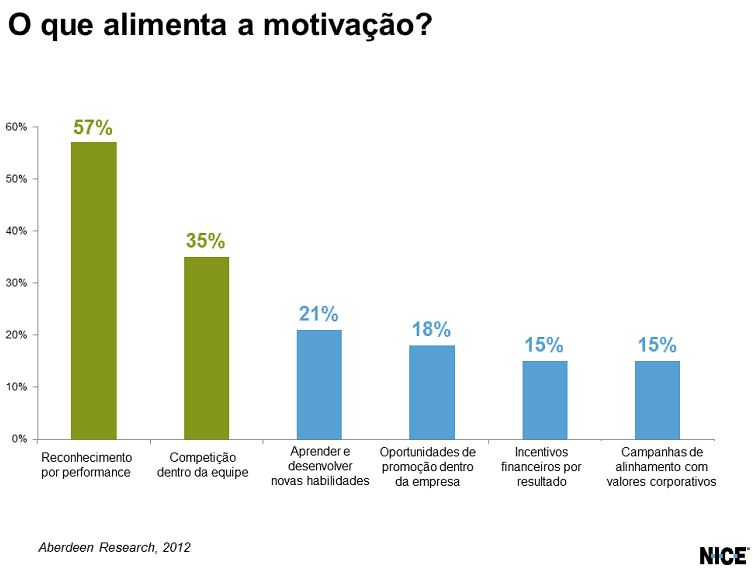
\includegraphics[width=16cm]{imagens/recompensa.jpg}
	\caption{\label{fig:recompensa}O que alimenta a motivação?}
	\fonte{\cite{grafico-motivacao:2012}}
\end{figure}
\FloatBarrier

Além do reconhecimento ser uma grande solução para motivar um indivíduo, pode-se ver na \autoref{fig:recompensa} que outro método bastante efetivo é através da competitividade. Esta por sua vez, não tem a necessidade de ser estimulada diretamente, como ao promover um vencedor em um jogo. O fato de simplesmente parabenizar as melhores notas de uma turma em uma prova ou atividade, por exemplo, já é o suficiente para gerar um certo nível de competição de forma saudável. Fora o fato de que competições, quando são realizadas em grupos, podem ser importantes fatores para reforçar o trabalho em equipe \cite{gamificação-na-ead:2014}.



\chapter{Gerenciamento do Projeto}
Neste capítulo, são abordadas as informações a respeito do gerenciamento do projeto, como a metodologia de gestão adotada, a organização da equipe, a gestão do tempo e as métricas levantadas ao longo do projeto.

\section{Metodologia de Gestão}
A metodologia de gerenciamento de projeto adotada é o \textit{Scrum}.

O \textit{Scrum} é um \textit{\gls{framework}} para gestão de projetos que tem como principais objetivos agilizar o processo de desenvolvimento de \textit{\gls{software}} e responder rapidamente às mudanças. Ela é composta por cerimônias e tem como um dos pilares as \textit{\glspl{sprint}}, ou seja, um conjunto de atividades para um determinado tempo. 

Essa metodologia foi adotada devido à experiência da maioria dos integrantes da equipe, que utilizam esse \textit{\gls{framework}} no ambiente de trabalho, e também por ser uma metodologia que demonstra ser eficaz para um gerenciamento de projetos.


No caso do projeto, as atividades de uma \textit{\gls{sprint}} são planejadas em uma \textit{Sprint Planning}, que é a primeira cerimônia e tem como principal objetivo a definição das atividades até o final da \textit{\gls{sprint}}. Nessa cerimônia, baseando-se nas histórias priorizadas no \textit{Product Backlog} e nas pontuações de cada atividade, é criado o \textit{Sprint Backlog} para a respectiva \textit{\gls{sprint}}. E para auxiliar na visualização das tarefas e melhor controle das entregas, foi utilizado, para a criação do Sprint Backlog, o Kanban do GitHub, no qual possui três colunas: uma de To Do (a fazer), outra de Doing (fazendo) e outra de Done (feito). 


Após o planejamento da \textit{\gls{sprint}}, a execução das atividades é iniciada. Assim, reuniões semanais de acompanhamento são feitas para ver o andamento do projeto, alinhamento das expectativas da \textit{\gls{sprint}} e identificação de possíveis impedimentos. Desse modo, esses \textit{\glspl{checkpoint}} semanais acontecem todas as terças-feiras às 19:30 ao longo da \textit{\gls{sprint}}. 

No último dia da \textit{\gls{sprint}}, às 19h30, é feita uma reunião para revisão das entregas, a chamada \textit{Sprint Review}, na qual é identificado o que foi entregue com sucesso, o que não foi concluído e também possíveis mudanças no \textit{\gls{product-backlog}}. 


Após a \textit{Sprint Review}, é feita uma reunião de retrospectiva, a \textit{Sprint Retrospective}, para avaliar o desempenho da equipe, o andamento do projeto e possíveis melhorias para a próxima \textit{\gls{sprint}}. E logo em seguida, a \textit{Sprint Planning} da \textit{\gls{sprint}} seguinte é realizada.


Todas as reuniões acontecem através do \textit{Google Meet}.
E para eventuais dúvidas, alinhamentos e possíveis urgências é utilizado o \textit{WhatsApp} e, caso houver necessidade, reuniões no \textit{Google Meet}. 


\section{Organização da Equipe}
As atividades foram divididas entre os integrantes da equipe segundo as habilidades e interesses de cada um, levando-se em consideração também o nível de dificuldade de cada frente.


Desse modo, o André é o \textit{\gls{tech-lead}} da equipe e foca na frente de desenvolvimento do sistema, portanto a parte de preparação do ambiente, desenvolvimento \textit{\gls{back-end}} e \textit{\gls{front-end}} são as suas principais atividades, mas também atuou na elaboração da documentação, na fase inicial do projeto, e como suporte, ao longo dele.

A Bianca é a gerente de projetos e \textit{\gls{scrum-master}} da equipe, sendo a responsável por garantir as entregas do projeto, por subir os arquivos no \ac{svn}, por ser a facilitadora em possíveis conflitos e impedimentos que possam surgir. Tem como principal foco a elaboração da documentação, além de ser responsável também pelas postagens semanais no blog.

O Luiz auxilia na elaboração da documentação, sendo, portanto, o seu principal foco, mas também auxiliou na frente de desenvolvimento do \textit{\gls{front-end}}, na elaboração de protótipos de alta e baixa fidelidade do sistema.

O Natan também compõe o time de desenvolvimento, auxiliando no desenvolvimento do \textit{\gls{back-end}} e do \textit{\gls{front-end}}. É o responsável pela criação, edição e postagem dos vídeos, mas também auxilia na elaboração da documentação, sobretudo na sua conversão para o LaTeX, e na subida dos arquivos no \ac{svn}.

A Patrícia é a \textit{\gls{product-owner}} da equipe, tendo como principal foco a documentação, lidando também com o \textit{\gls{product-backlog}} e elicitação de requisitos. Ela também auxilia na frente do desenvolvimento \textit{\gls{front-end}}, sobretudo na parte de protótipos de telas, testes e estilização das telas. 

Como uma das equipes da sala foi desfeita três semanas antes da entrega do \ac{mvp}, os integrantes que continuaram na disciplina foram alocados nas demais equipes. Foi nesse contexto que o Gustavo passou a integrar a equipe, fazendo parte do time de desenvolvimento e auxiliando tanto no desenvolvimento \textit{\gls{back-end}} quanto no \textit{\gls{front-end}}.

\section{Gestão de Tempo}

Baseando-se no Scrum, a gestão do tempo será feita pelas \textit{\glspl{sprint}}. Cada \textit{\gls{sprint}} terá a duração de duas semanas e, no total, serão quinze \textit{\glspl{sprint}}, com previsão de datas de início e de fim conforme descrito no \autoref{quadro-sprints}. 


\begin{quadro}[htb]
\centering
\ABNTEXfontereduzida
\caption{\label{quadro-sprints}Data de início e data fim de cada
\textit{sprint}}
\begin{tabular}{|c|c|c|}
   \hline
   \thead{Sprint} & \thead{Data Início}  & \thead{Data Fim}   \\\hline
    1 & 10/05/21 & 25/05/21 \\\hline
    2 & 25/05/21 & 08/06/21 \\\hline
    3 & 08/06/21 & 22/06/21 \\\hline
    4 & 22/06/21 & 06/07/21 \\\hline
    5 & 06/07/21 & 20/07/21 \\\hline
    6 & 20/07/21 & 03/08/21 \\\hline
    7 & 03/08/21 & 17/08/21 \\\hline
    8 & 17/08/21 & 31/08/21 \\\hline
    9 & 31/08/21 & 14/09/21 \\\hline
    10 & 14/09/21 & 28/09/21 \\\hline
    11 & 28/09/21 & 12/10/21 \\\hline
    12 & 12/10/21 & 26/10/21 \\\hline
    13 & 26/10/21 & 09/11/21 \\\hline
    14 & 09/11/21 & 23/11/21 \\\hline
    15 & 23/11/21 & 14/12/21 \\\hline
\end{tabular}
\fonte{Os autores}
\end{quadro}
\FloatBarrier

Com a definição das datas para cada \textit{\gls{sprint}}, foi possível elaborar um gráfico de Gantt para o projeto. A \autoref{cronograma} demonstra as entregas esperadas para cada \textit{\gls{sprint}}.


\begin{PAGINA-A3}

\begin{figure}[p]
    \centering 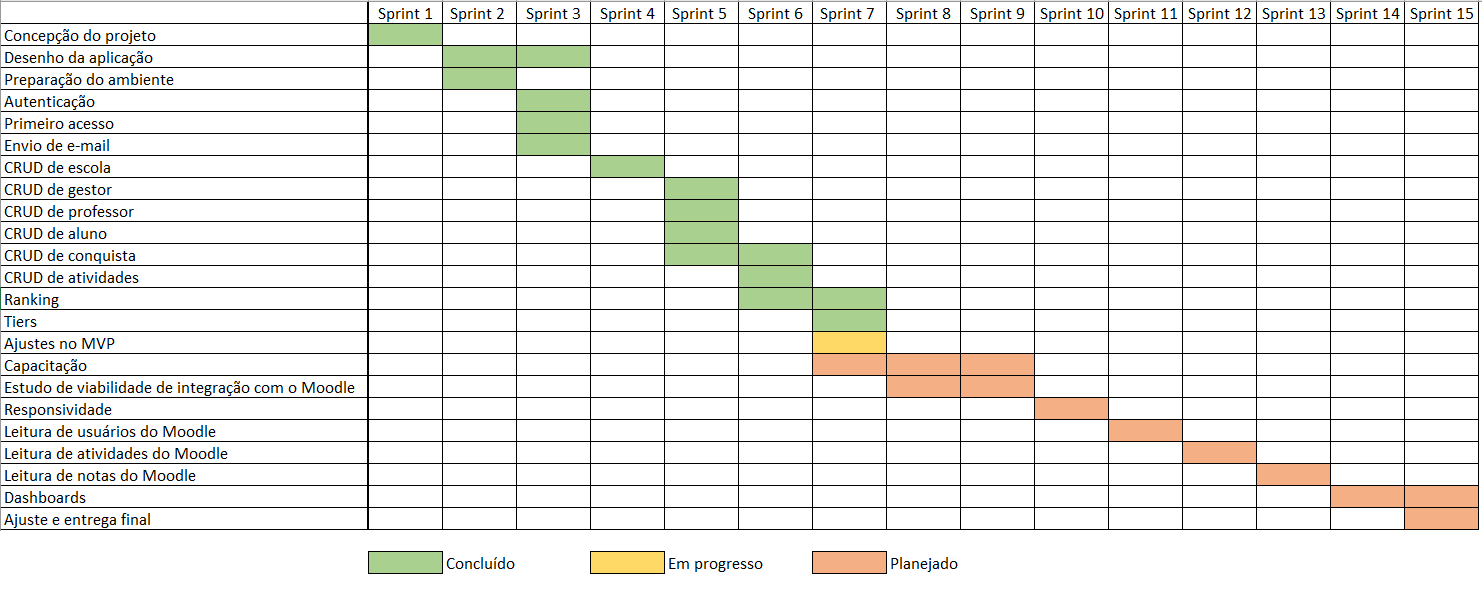
\includegraphics[height=\textheight,width=\textwidth,keepaspectratio]{imagens/Cronograma.png}
	\caption{\label{cronograma}Gráfico de Gantt}
   \fonte{Os autores}
\end{figure}

\end{PAGINA-A3}

As atividades de cada uma das \textit{\glspl{sprint}} planejadas podem ser visualizadas no \autoref{sprints-atividades}.


\section{Métricas}
Uma vez por mês, foram levantados métricas cumulativas a respeito do andamento do projeto. O \autoref{quadro-metricas} representa os resultados obtidos.
\begin{quadro}[htb]
\centering
\ABNTEXfontereduzida
\caption{\label{quadro-metricas}Métricas Gerais}
\begin{tabular}{|c|c|c|c|c|}
   \hline
   \thead{Métricas} & \thead{Maio}\footnote{Começo em 10 de maio} & \thead{Junho}  & \thead{Julho} & \thead{Agosto}\footnote{Medido até dia 08 de agosto}   \\\hline
    Reuniões & 5 & 10 & 15 & 16\\\hline
    Vídeos & 1 & 4 & 7 & 7 \\\hline
    Publicações no blog & 3 & 7 & 12 & 14 \\\hline
    Arquivos na pasta do SVN & 11 & 99 & 486 & 546 \\\hline
    Commits & 3 & 25 & 108 & 225 \\\hline
    Entidades no back-end & 1 & 2 & 11 & 15 \\\hline
    Linhas de código & 13 & 15859 & 112453 & 168757\\\hline
\end{tabular}
\fonte{Os autores}
\end{quadro}
\FloatBarrier

\subsection{StatSVN}
A ferramenta \textit{StatSVN} foi utilizada para extrair relatórios a respeito do histórico do repositório da equipe no \gls{svn} e assim pôde-se obter dados estatísticos a respeito do desenvolvimento do projeto.

As Figuras \ref{fig:activity} e \ref{fig:commitsauthors} demonstram, respectivamente, as atividades dos integrantes da equipe e os \textit{commits} realizados por eles. Com esses gráficos, torna-se evidente que apenas a Bianca e o Natan atualizaram o repositório. Isso aconteceu porque a principal ferramenta usada para o versionamento de código foi o \textit{GitHub}, mas como o \gls{svn} é um dos requisitos para a disciplina, eles ficaram responsáveis por atualizar o repositório. Ao final do período, o Luiz passou a ajudar na subida dos arquivos em LaTeX para o \gls{svn}.
\begin{figure}[htb]
    \centering
	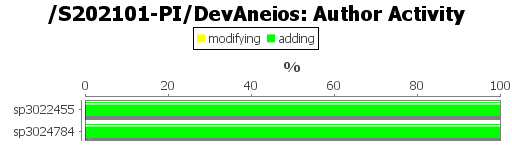
\includegraphics[width=16cm]{imagens/activity.png}
	\caption{\label{fig:activity} Atividades dos integrantes}
	\fonte{Os autores}
\end{figure}
\FloatBarrier

\begin{figure}[htb]
    \centering
	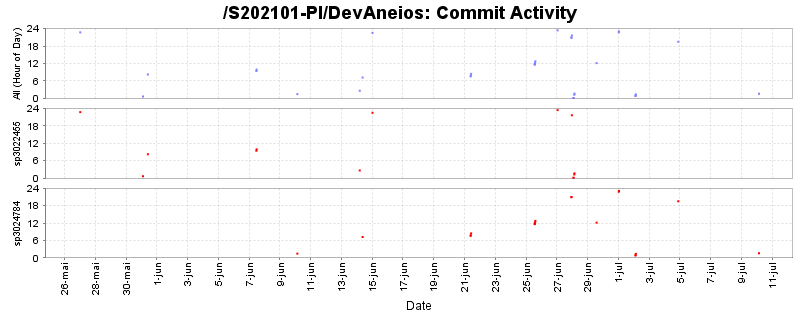
\includegraphics[width=16cm]{imagens/commitscatterauthors.png}
	\caption{\label{fig:commitsauthors} Commits por autor}
	\fonte{Os autores}
\end{figure}
\FloatBarrier

A \autoref{fig:day} demonstra os \textit{commits} da equipe por dia da semana. Com esse gráfico, é possível notar que os dias que mais foram realizados \textit{commits} foram na terça-feira e segunda-feita, que representam os dias que acontecem os \textit{checkpoints} semanais da equipe e as entregas da disciplina, respectivamente.

\begin{figure}[htb]
    \centering
	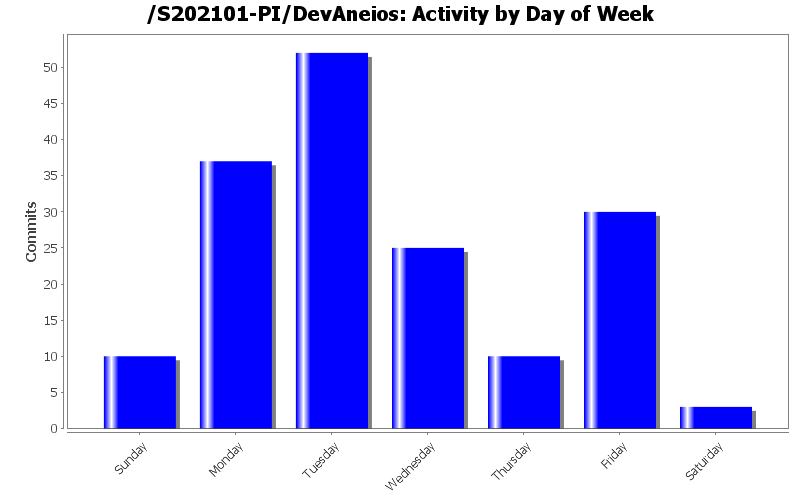
\includegraphics[width=16cm]{imagens/activity_day.png}
	\caption{\label{fig:day} Atividades por dia na semana}
	\fonte{Os autores}
\end{figure}
\FloatBarrier

A \autoref{fig:time} demonstra os \textit{commits} da equipe por horas do dia. Com esse gráfico, é possível verificar que os horários que mais foram feitos \textit{commits} foram de madrugada e na hora do almoço, representado os horários do dia que os integrantes tinham mais disponibilidade para se dedicar ao projeto.

\begin{figure}[htb]
    \centering
	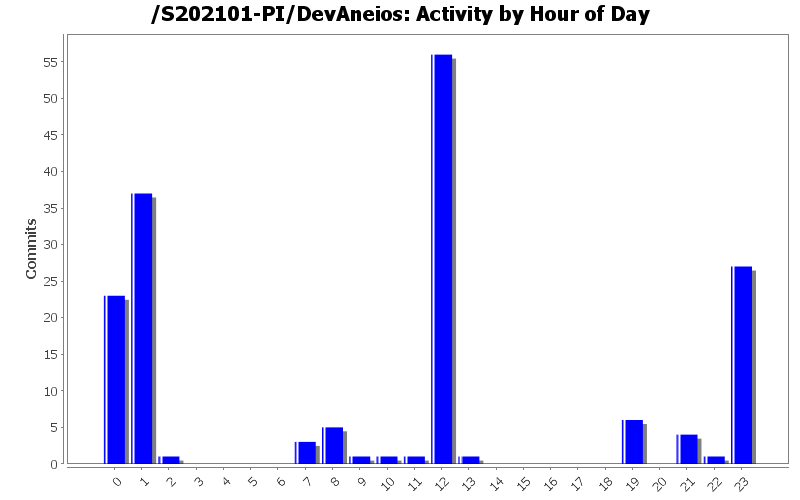
\includegraphics[width=16cm]{imagens/activity_time.png}
	\caption{\label{fig:time} Atividades por hora no dia}
	\fonte{Os autores}
\end{figure}
\FloatBarrier

A \autoref{fig:loc} demonstra a quantidade de linhas de código pelos dias ao longo dos meses. Com esse gráfico, é possível observar elevadas curvas de crescimento espaçadas, demonstrando os dias que o repositório era atualizado.

\begin{figure}[htb]
    \centering
	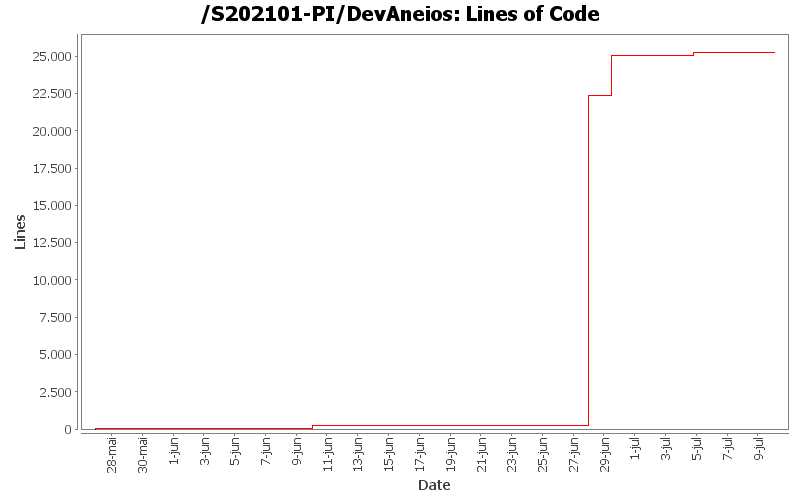
\includegraphics[width=16cm]{imagens/loc.png}
	\caption{\label{fig:loc} Linhas de código}
	\fonte{Os autores}
\end{figure}
\FloatBarrier

\subsection{\textit{GitHub}}
Como o \textit{GitHub} foi a principal ferramenta para versionamento do código, convém demonstrar as métricas geradas por ele. As Figuras \ref{git-backend} e \ref{git-frontend} representam, respectivamente, as métricas do repositório do \textit{\gls{back-end}} e do repositório do \textit{\gls{front-end}}.

\begin{figure}[htb]
    \centering
	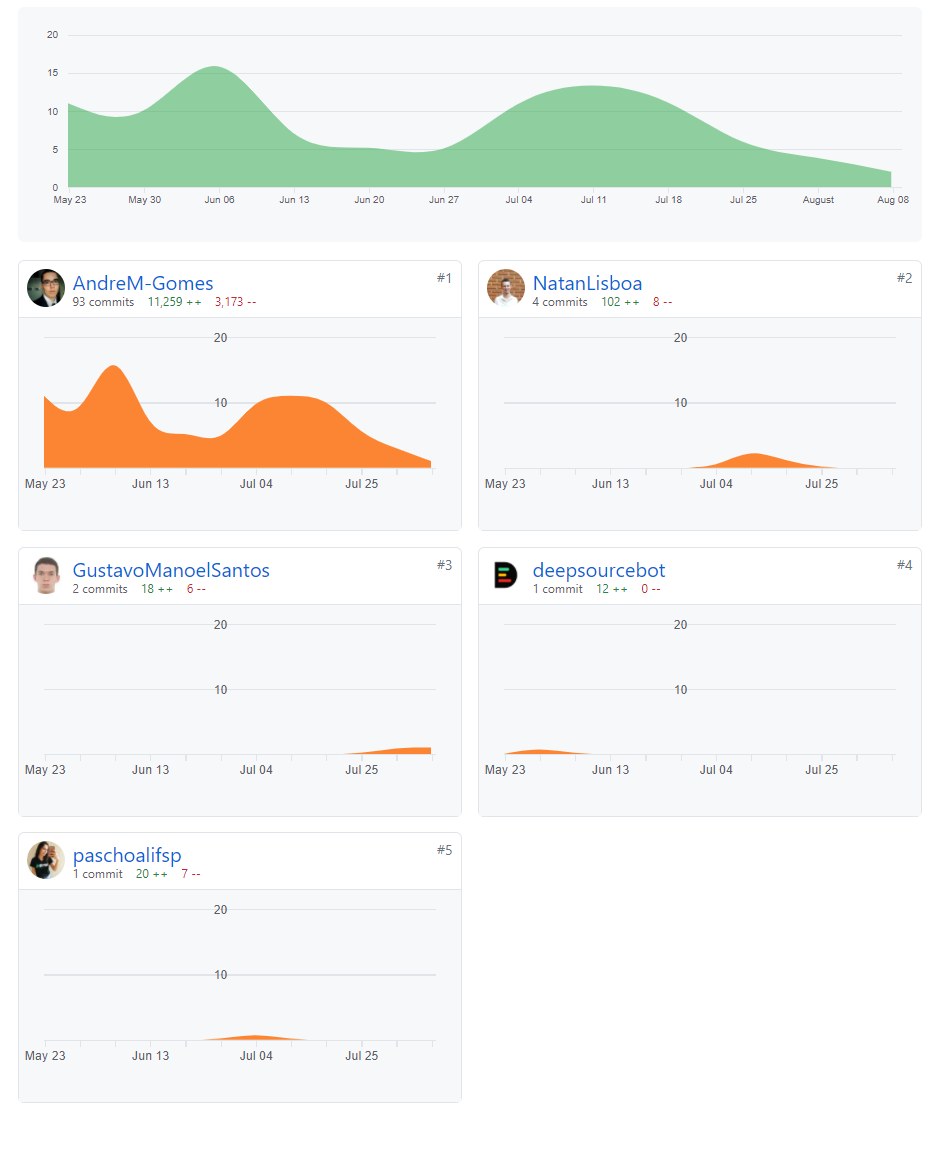
\includegraphics[width=16cm]{imagens/MetricasGitBack.png}
	\caption{\label{git-backend} Métricas do repositório do \textit{back-end} geradas pelo GitHub}
	\fonte{Os autores}
\end{figure}
\FloatBarrier


\begin{figure}[htb]
    \centering
	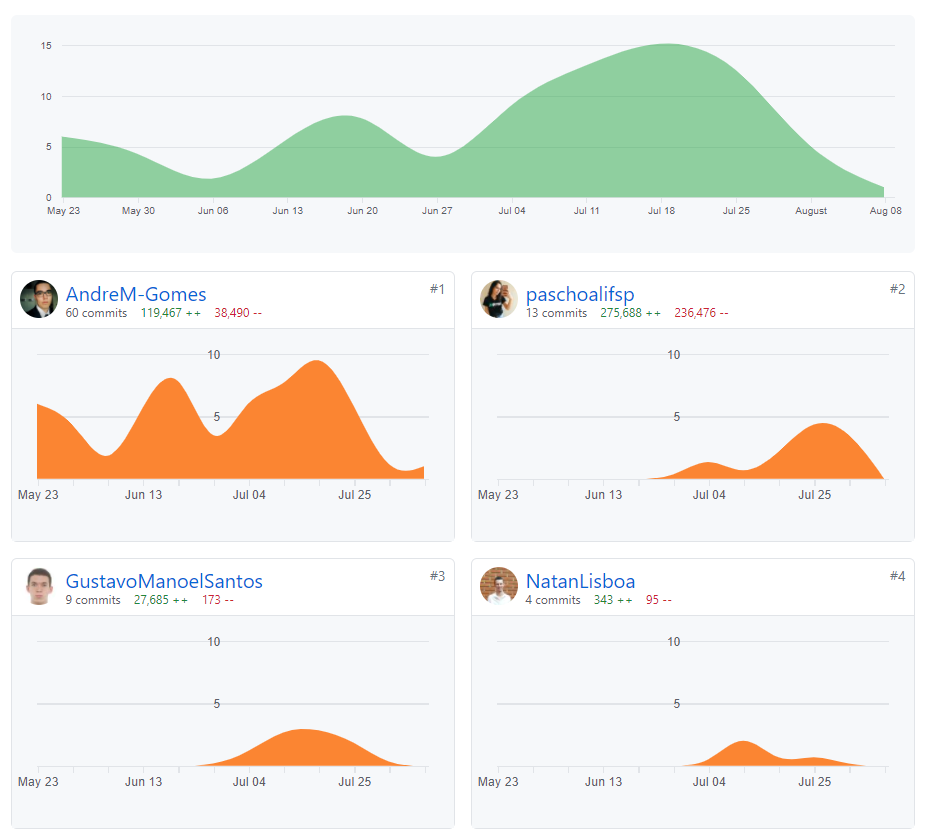
\includegraphics[width=16cm]{imagens/MetricasGitFront.png}
	\caption{\label{git-frontend} Métricas do repositório do \textit{front-end} geradas pelo GitHub}
	\fonte{Os autores}
\end{figure}
\FloatBarrier

Com os gráficos, torna-se nítido que o André foi a pessoa quem mais desenvolveu ao longo do tempo, sobretudo devido ao fato de esse ser o seu principal foco desde o começo e por apresentar um conhecimento técnico superior aos demais integrantes da equipe. A Patrícia cuidou mais da parte do \textit{\gls{front-end}}, sobretudo da cobertura de testes. E o Natan e o Gustavo auxiliaram na resolução de \textit{bugs} que apareciam.

\section{Links de acesso}

Os \textit{\glspl{link}} de acesso pertinentes ao projeto estão disponíveis nesta seção.

A \autoref{qr-github} contém o \textit{\gls{qr-code}} que leva ao principal repositório remoto utilizado para o versionamento de código durante o desenvolvimento da aplicação, o \textit{GitHub}.
A fim de obter uma melhor divisão lógica, foram criados dois repositórios na plataforma para hospedar os códigos relacionados ao \textit{\gls{front-end}} e ao \textit{\gls{back-end}} do projeto.

\begin{figure}[htb]
\begin{flushright}
\begin{pspicture}(25mm,25mm)
\psbarcode{https://github.com/devaneios-ifsp}{eclevel=H width=1.0 height=1.0}{qrcode}
\end{pspicture}
\caption{\label{qr-github}\textit{QR-Code} - Repositório remoto GitHub}
\legend{\url{https://github.com/devaneios-ifsp}}
\fonte{Os Autores}
\end{flushright}
\end{figure}
\FloatBarrier


Além do GitHub, o repositório Subversion também foi utilizado para gerenciamento do código produzido, sendo atualizado periodicamente. A \autoref{qr-svn} contém o \textit{\gls{qr-code}} do repositório em questão.

\begin{figure}[htb]
%\begin{flushright}
\begin{pspicture}(25mm,25mm)
\psbarcode{https://svn.spo.ifsp.edu.br/viewvc/A6PGP/S202101-PI/DevAneios/}{eclevel=H width=1.0 height=1.0}{qrcode}
\end{pspicture}
\caption{\label{qr-svn}\textit{QR-Code} - Repositório remoto Subversion}
\legend{\url{https://svn.spo.ifsp.edu.br/viewvc/A6PGP/S202101-PI/DevAneios/}}
\fonte{Os Autores}
%\end{flushright}
\end{figure}
\FloatBarrier

Todos os vídeos produzidos pela equipe podem ser acessados no canal do Youtube da mesma, cujo \gls{link} está contido no \textit{\gls{qr-code}} da \autoref{qr-yt}.

\begin{figure}[htb]
\begin{flushright}
\begin{pspicture}(25mm,25mm)
\psbarcode{https://www.youtube.com/channel/UCjwYXnZHuCg74AkhR5aZs6A/featured}{eclevel=H width=1.0 height=1.0}{qrcode}
\end{pspicture}
\caption{\label{qr-yt}\textit{QR-Code} - Canal DevAneios no Youtube}
\legend{\url{https://www.youtube.com/channel/UCjwYXnZHuCg74AkhR5aZs6A/featured}}
\fonte{Os Autores}
\end{flushright}
\end{figure}
\FloatBarrier

Os relatórios semanais de atividades realizadas por cada membro do projeto são publicadas no blog da equipe, cujo \gls{link} pode ser acessado no \textit{\gls{qr-code}} da \autoref{qr-blog}.

\begin{figure}[htb]
%\begin{flushright}
\begin{pspicture}(25mm,25mm)
\psbarcode{https://devaneiosifsp.blogspot.com/}{eclevel=H width=1.0 height=1.0}{qrcode}
\end{pspicture}
\caption{\label{qr-blog}\textit{QR-Code} - Blog DevAneios}
\legend{\url{https://devaneiosifsp.blogspot.com/}}
\fonte{Os Autores}
%\end{flushright}
\end{figure}
\FloatBarrier

A página de login e cadastramento do site Turma de Elite pode ser acessada através do {\gls{qr-code}} na \autoref{qr-login}, com as credenciais informadas.

\begin{figure}[htb]
\begin{flushright}
\begin{pspicture}(25mm,25mm)
\psbarcode{https://turma-de-elite-app.web.app/login}{eclevel=H width=1.0 height=1.0}{qrcode}
\end{pspicture}
\caption{\label{qr-login}\textit{QR-Code} - Tela de Login Turma de Elite}
\legend{\url{https://turma-de-elite-app.web.app/login}}
\fonte{Os Autores}
\end{flushright}
\end{figure}
\FloatBarrier

Para acessar a aplicação, usar o seguinte e-mail e senha:
\begin{itemize}
    \item E-mail: andre.montero702@gmail.com
    \item Senha: 123456
\end{itemize}

Os detalhes da API do projeto são documentados na aplicação Swagger. Seu \gls{link} de acesso pode ser encontrado através do {\gls{qr-code}} da \autoref{qr-swagger}.

\begin{figure}[htb]
%\begin{flushright}
\begin{pspicture}(25mm,25mm)
\psbarcode{https://turma-de-elite.herokuapp.com/swagger-ui/}{eclevel=H width=1.0 height=1.0}{qrcode}
\end{pspicture}
\caption{\label{qr-swagger}\textit{QR-Code} - Swagger do Turma de Elite}
\legend{\url{https://turma-de-elite.herokuapp.com/swagger-ui/}}
\fonte{Os Autores}
%\end{flushright}
\end{figure}
\FloatBarrier

\chapter{Desenvolvimento do Projeto}
Neste capítulo, são abordadas as informações a respeito do desenvolvimento do projeto, como a sua arquitetura, escopo, tecnologias utilizadas, manutenibilidade, quesitos de segurança, viabilidade financeira, escolhas e descartes do projeto.

\section{Arquitetura de solução}

A arquitetura da solução é baseada, de uma forma geral, na arquitetura \ac{mvc}. Este modelo é apresentado em camadas que separam a apresentação e a interação de dados no sistema. É estruturado em três componentes: o modelo, que é o responsável pelo gerenciamento dos dados, a visão, que gerencia a apresentação dos dados, e o controlador, responsável por intermediar a comunicação entre os eventos gerados pelo usuário na interface e o modelo \cite{engenharia-de-software:2018}.

O diagrama apresentado pela \autoref{fig:arquitetura}, mostra o modelo arquitetural.

\begin{figure}[htb]
    \centering
	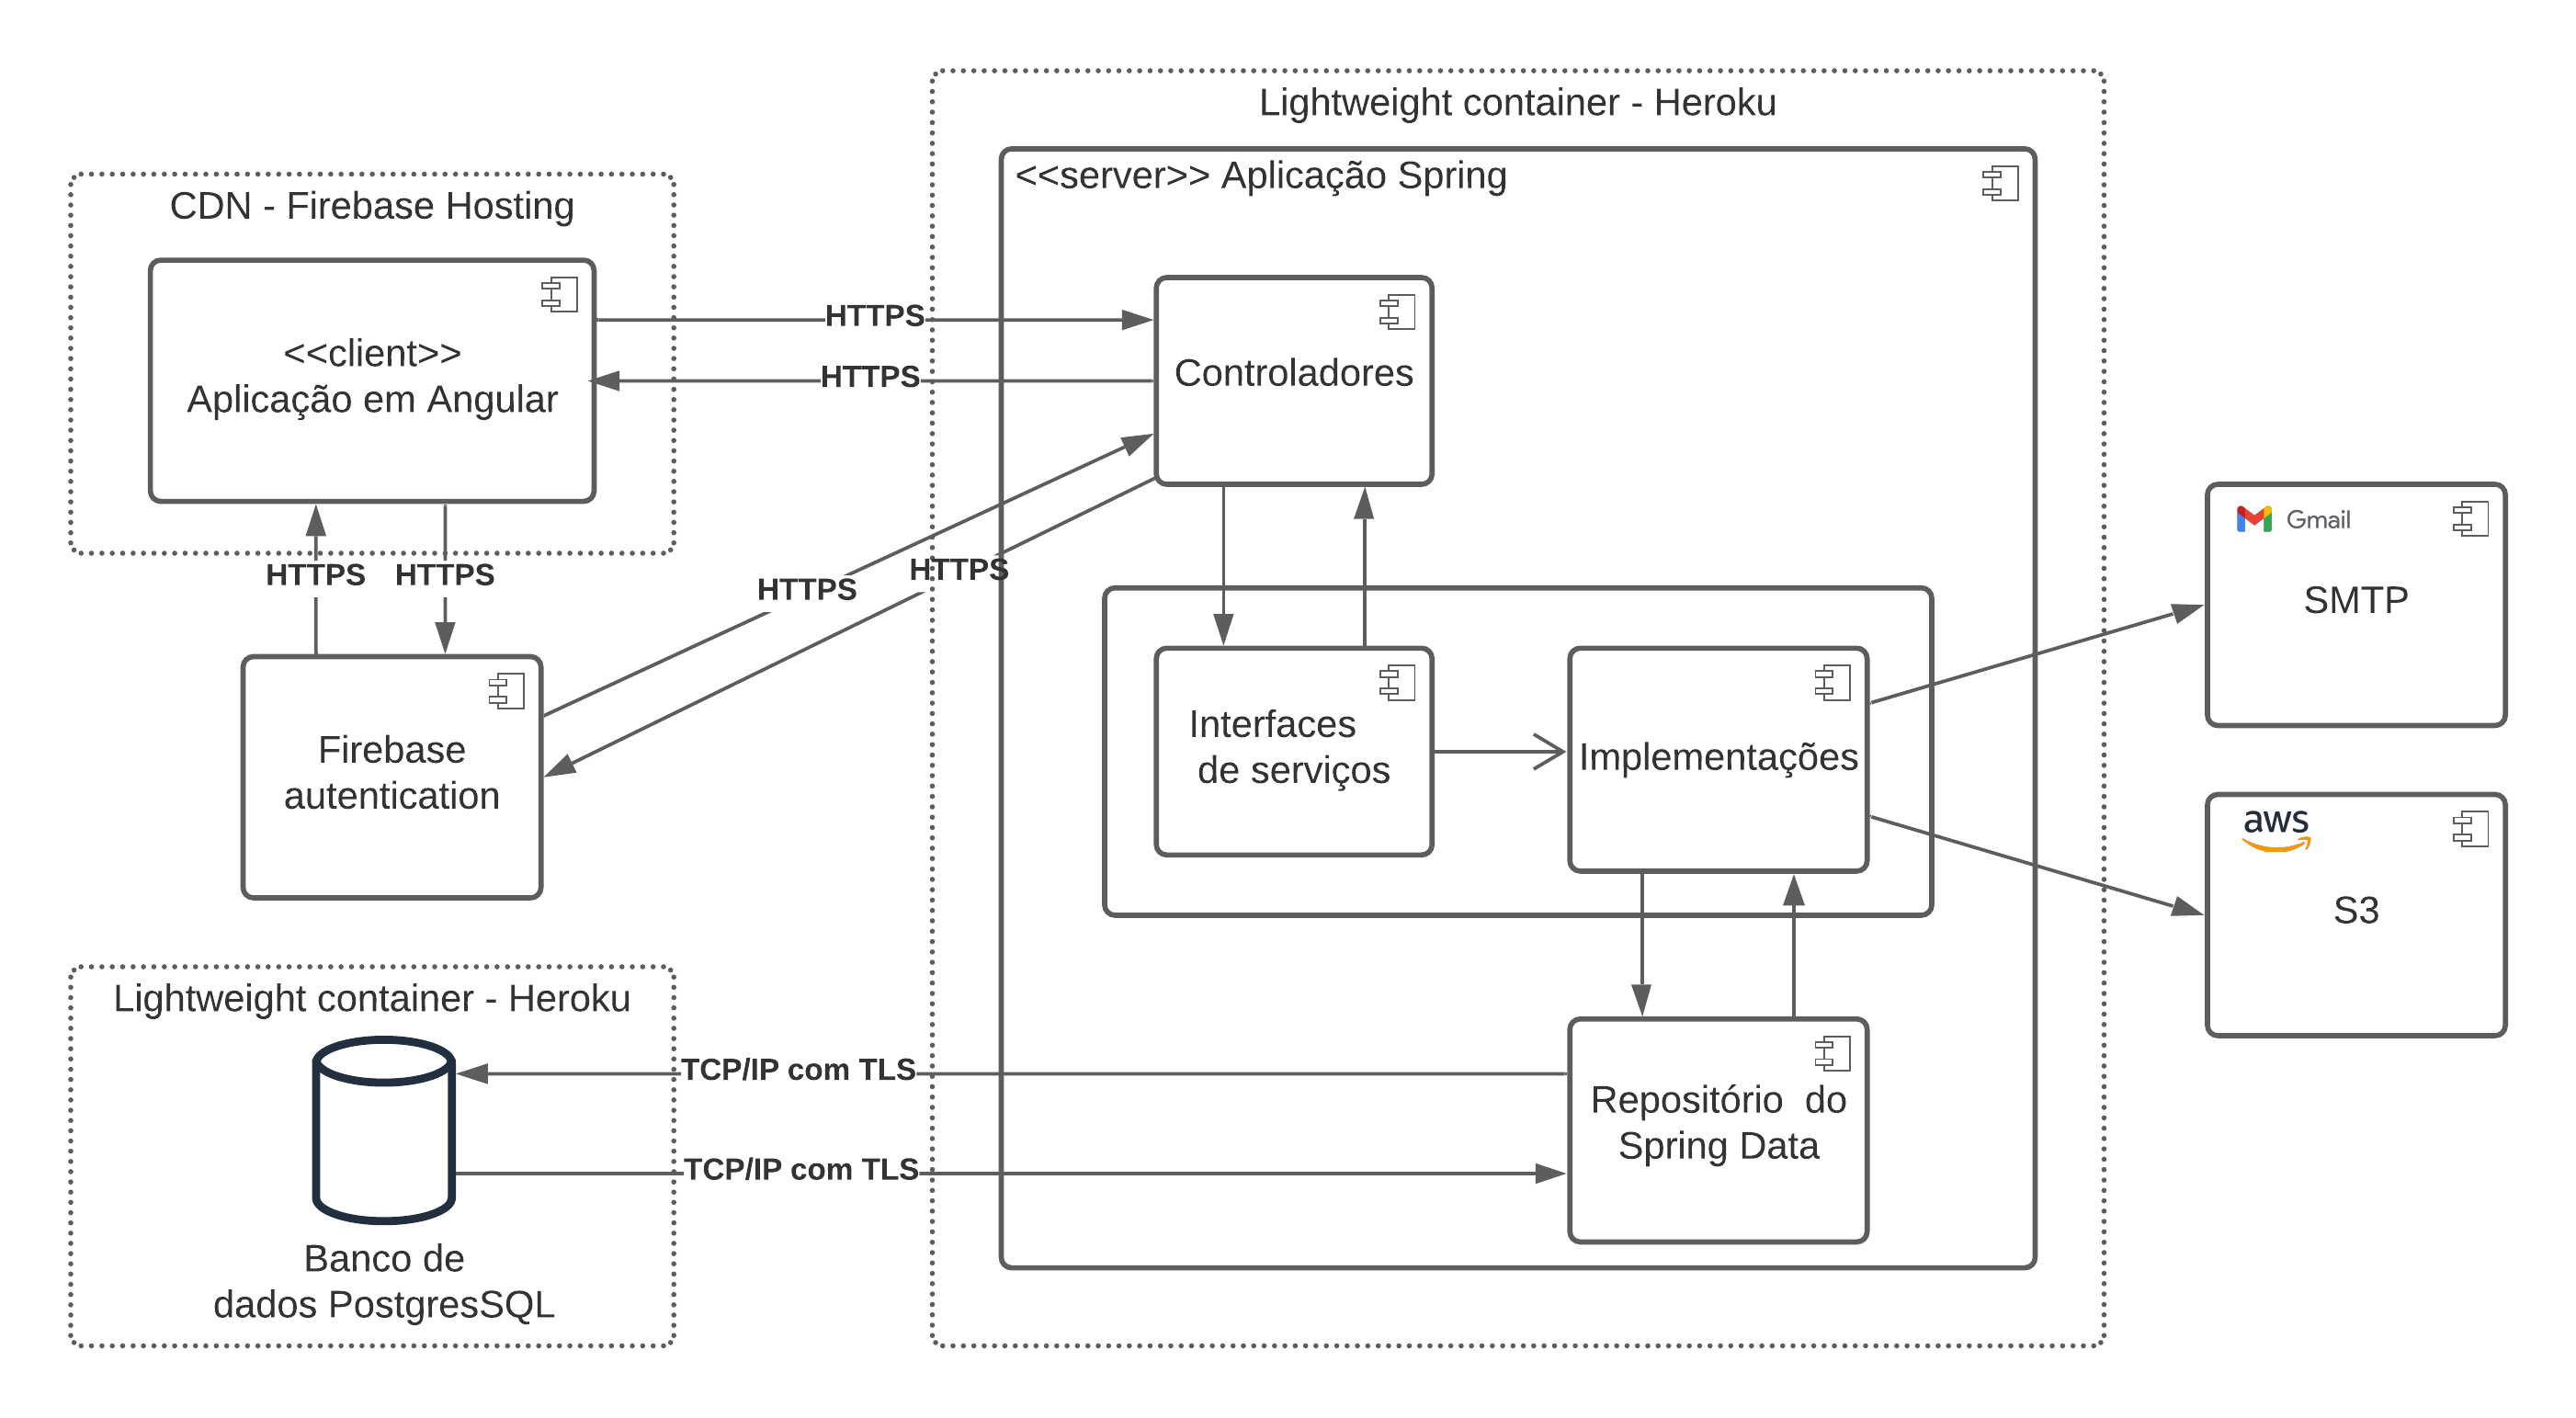
\includegraphics[width=16cm]{imagens/Arquitetura.png}
	\caption{\label{fig:arquitetura} Arquitetura da solução}
	\fonte{Os autores}
\end{figure}
 
 
De modo a desenvolver uma aplicação que busca garantir uma boa usabilidade e capaz de aproveitar os recursos disponíveis da melhor forma, para a interface do usuário (\textit{\gls{front-end}}) será adotado o modelo arquitetural \ac{spa}. 


Neste modelo, a maioria dos recursos necessários é carregada na inicialização da aplicação, fazendo com que não seja necessário recarregar a página durante o uso. A única mudança que ocorre é a dos dados, que são trafegados entre o servidor e o cliente.


Conforme o diagrama apresentado pela \autoref{fig:arquitetura}, as camadas que compõem a solução utilizam as seguintes infraestruturas para hospedagem:
\begin{itemize}
\item \ac{cdn} (Firebase Hosting): infraestrutura responsável por hospedar a aplicação em Angular, da camada de visão. Um serviço de hospedagem, que tem como base o armazenamento em \ac{ssd} e uma \ac{cdn}, totalmente gerenciado para conteúdo estático e dinâmico.
\item  Lightweight container (Heroku): infraestrutura responsável por hospedar a aplicação Spring da camada controladora e o banco de dados da camada de modelo. A tecnologia utilizada pelo Heroku, utiliza o conceito de \textit{\gls{container}} que empacota o código e as dependências do aplicativo abstraindo o gerenciamento do \textit{\gls{hardware}}, levando a simplificação do desenvolvimento e o aumento da produtividade.
\end{itemize}

Para a autenticação da aplicação, é utilizado o Firebase Authentication. E para minimizar os impactos negativos da utilização de uma tecnologia terceira, o Firebase Authentication é implantado seguindo o padrão de projeto \textit{Adapter}. Deste modo, diante da necessidade, a tecnologia pode ser facilmente substituída por outra ou até mesmo por uma proprietária.

Para finalizar a composição da arquitetura da aplicação foram adicionadas duas implementações. O \ac{smtp} do Gmail, protocolo responsável por apoiar o envio e-mails da aplicação. E o S3 da Aws, serviço responsável pelo armazenamento dos documentos de atividades.


A comunicação entre a camada de visão e a camada controladora será realizada via protocolo \ac{https}. Este protocolo acrescenta uma camada a mais de segurança à aplicação, uma vez que utiliza a criptografia na transferência de recursos.


Já a comunicação entre os controladores e banco de dados, é realizada via \ac{tcpip} acrescido do protocolo \ac{tls} que aumenta a segurança através de criptografia, a interoperabilidade, a extensibilidade e a eficiência.




\section{Escopo do Projeto}
A proposta de projeto é uma aplicação \textit{web} voltada para auxiliar no acompanhamento da evolução no rendimento dos alunos nas atividades escolares. 

\subsection{Modelagem}
Para detalhar melhor a aplicação, foi feita a análise de requisitos, a elaboração das histórias de usuários, a criação do backlog do produto, a modelagem de dados e elaboração dos protótipos.

\subsubsection{Análise de Requisitos}
A análise de requisitos é fundamental para o desenvolvimento da aplicação, pois a partir dela pode ser levantadas as funcionalidades e restrições que o sistema deve apresentar. Para isso, foram levantados os requisitos funcionais e não funcionais do sistema.

\subsubsubsection{Requisitos Funcionais}
Os requisitos funcionais levantados são descritos no \autoref{quadro-requisitosfuncionais}.
\begin{quadro}[htb]
\centering
\ABNTEXfontereduzida
\caption{\label{quadro-requisitosfuncionais}Requisitos funcionais}
\begin{tabular}{|m{2.2cm}|m{9.6cm}|m{2.2cm}|}
\hline
{\thead{Identificador}} & \thead{Descrição} & \thead{Categoria}   \\ \hline
    RF01 &  O sistema deve permitir o cadastro de um administrador por outro administrador &  Essencial \\ \hline
    RF02 & O sistema deve permitir o cadastro de escola pelo administrador  & Essencial \\\hline
    RF03 & O sistema deve permitir o envio de e-mail para completar o cadastro de escola & Essencial  \\ \hline
    RF04 & O sistema deve permitir a visualização de um resumo do uso do sistema para o administrador & Importante  \\ \hline
    RF05 & O sistema deve permitir uma definição de senha no primeiro acesso &  Essencial   \\ \hline
    RF06 &  O sistema deve permitir a realização do login & Essencial \\ \hline  
    RF07 &  O sistema deve permitir a recuperação de senha &  Essencial \\ \hline 
    RF08 &  O sistema deve permitir a revogação o acesso de um administrador e de um gestor &  Essencial  \\ \hline   
    RF09 &  O sistema deve permitir a desativação de uma escola &  Essencial \\ \hline
    RF10 &  O sistema deve permitir o cadastro de turmas pelo gestor & Essencial  \\ \hline    
    RF11 &  O sistema deve permitir o cadastro de professores pelo gestor & Essencial  \\ \hline    
    RF12 &  O sistema deve permitir a atribuição de um ou mais professores e seus respectivos alunos às turmas &  Essencial \\ \hline  
    RF13 & O sistema deve permitir ao professor somente a exibição das turmas atribuídas ao mesmo  & Essencial \\ \hline 
    RF14 &  O sistema deve permitir o cadastro de atividades pelo professor & Essencial  \\ \hline  
    RF15 &  O sistema deve permitir o detalhamento das atividades & Essencial  \\ \hline  
    RF16 & O sistema deve permitir ao professor somente a exibição das atividades das turmas atribuídas ao mesmo  & Essencial \\ \hline  
    RF17 &  O sistema deve permitir a entrega e visualização das atividades &  Essencial \\ \hline  
    RF18 &  O sistema deve permitir a visualização e atribuição de correções & Essencial  \\ \hline  
    RF19 &  O sistema deve permitir o cadastro de conquistas pelo professor &  Essencial \\ \hline  
    RF20 &  O sistema deve permitir a listagem de conquistas personalizada para cada perfil & Essencial  \\ \hline  
    RF21 &  O sistema deve permitir a visualização do ranking personalizada para cada perfil &  Essencial \\ \hline  
    RF22 &  O sistema deve permitir o cálculo e visualização de pontuações &  Essencial \\ \hline  
    RF23 &  O sistema deve permitir o detalhamento das conquistas & Essencial  \\ \hline  
    RF24 &  O sistema deve permitir a visualização de dashboards para acompanhar o desempenho & Importante  \\ \hline  
    RF25 &  O sistema deve permitir a utilização dos conceitos de gamificação presentes nessa aplicação, em outras aplicações &  Importante \\ \hline  

\end{tabular}
\fonte{Os autores}
\end{quadro}
\FloatBarrier

\subsubsubsection{Requisitos Não Funcionais}
Os requisitos não funcionais levantados são descritos no \autoref{quadro-requisitosnaofuncionais}.
\begin{quadro}[htb]
\centering
\ABNTEXfontereduzida
\caption{\label{quadro-requisitosnaofuncionais}Requisitos não funcionais}
\begin{tabular}{|m{2.2cm}|m{9.6cm}|m{2.2cm}|}
\hline
{\thead{Identificador}} & \thead{Descrição} & \thead{Categoria}   \\ \hline
    RNF01 & O sistema deve possuir telas responsivas &  Usabilidade \\ \hline
    RNF02 & O sistema deve seguir o protocolo HTTPS & Segurança \\\hline
    RNF03 & O sistema deve respeitar a LGPD & Segurança  \\ \hline
    RNF04 & O sistema deve permitir a sua escalabilidade no futuro & Desempenho  \\ \hline
    RNF05 & O sistema deve estar disponível sete dias por semana &  Disponibilidade   \\ \hline
\end{tabular}
\fonte{Os autores}
\end{quadro}
\FloatBarrier


\subsubsection{Histórias de Usuário}
Com os requisitos levantados, foi-se possível elaborar as histórias de usuário para estabelecer as funcionalidades do sistema. 

\begin{itemize}
    \item\textbf{Funcionalidade}: Cadastro de administrador
    
    Eu, como administrador, quero criar outro administrador, para que alguém possa me ajudar nas tarefas administrativas do sistema.
    \begin{itemize}
        \item Cenário: Cadastro bem sucedido  
        \par Dado que estou na tela de cadastro de usuários na visão do administrador
        \par Quando eu preencher todos os dados corretamente
        \par E apertar o botão de Criar
        \par Então receberei uma mensagem de usuário criado com sucesso
    \end{itemize}   
    \begin{itemize}
        \item Cenário: Cadastro mal sucedido  
        \par Dado que estou na tela de cadastro de usuários na visão do administrador
        \par Quando eu preencher algum dado incorretamente
        \par Então não conseguirei clicar no botão de Criar, pois o botão estará inativo
    \end{itemize}       

\item\textbf{Funcionalidade}: Cadastro de escola
    
    Eu, como administrador, gostaria de cadastrar escolas para meus clientes.
    \begin{itemize}
        \item Cenário: Cadastro bem sucedido  
        \par Dado que estou na tela de cadastro de escolas na visão do administrador
        \par Quando eu preencher todos os dados corretamente
        \par E apertar o botão de Criar
        \par Então receberei uma mensagem de escola criada com sucesso
    \end{itemize}   
    \begin{itemize}
        \item Cenário: Cadastro mal sucedido  
        \par Dado que estou na tela de cadastro de escolas na visão do administrador
        \par Quando eu preencher algum dado incorretamente
        \par Então não conseguirei clicar no botão de Criar
    \end{itemize}    

\item\textbf{Funcionalidade}: Envio de e-mail
    
    Eu, como administrador, gostaria que, ao criar uma escola, fosse enviado um e-mail para o gestor com uma página para que ele complemente as informações da escola e do seu usuário.
    \begin{itemize}
        \item Cenário: Envio de e-mail para cadastro de escola 
        \par Dado que estou na tela de escolas na visão do administrador
        \par Quando eu criar uma nova escola
        \par Então o gestor da escola receberá um e-mail para completar o cadastro de sua escola
    \end{itemize}    

\item\textbf{Funcionalidade}: Resumo do uso do sistema
    
    Eu, como administrador, quero visualizar um resumo do uso do sistema, para que eu possa tomar decisões com base no uso.
    \begin{itemize}
        \item Cenário: Visualização do uso do sistema 
        \par Dado que estou na tela de login
        \par Quando eu fazer o login com o perfil de administrador
        \par Então conseguirei ver o resumo do uso do sistema
    \end{itemize} 

\item\textbf{Funcionalidade}: Primeiro acesso
    
    Eu, como usuário do sistema, gostaria de poder definir a minha senha durante o primeiro acesso a aplicação para garantir a segurança do acesso.
    \begin{itemize}
        \item Cenário: Definição de senha  
        \par Dado que o meu usuário já está cadastrado
        \par E recebi o link de acesso à aplicação por e-mail
        \par Quando eu clicar nesse link
        \par E ser redirecionado à tela de primeiro acesso
        \par Então conseguirei definir a minha senha
    \end{itemize}

\item\textbf{Funcionalidade}: Login
    
    Eu, como usuário do sistema, gostaria de fazer o login na aplicação para garantir a privacidade dos meus dados.
    \begin{itemize}
        \item Cenário: Login bem sucedido  
        \par Dado que estou na tela de login
        \par Quando eu preencher o e-mail e a senha corretamente
        \par E apertar o botão de Login
        \par Então irei para a tela inicial da aplicação
    \end{itemize}   
    \begin{itemize}
        \item Cenário: Login mal sucedido  
        \par Dado que estou na tela de login
        \par Quando eu preencher algum dado incorretamente
        \par Então receberei uma mensagem de erro
    \end{itemize}    

\item\textbf{Funcionalidade}: Recuperação de senha
    
    Eu, como usuário do sistema, gostaria de poder recuperar minha senha.
    \begin{itemize}
        \item Cenário: Cadastro de nova senha
        \par Dado que estou na tela de login
        \par Quando eu clicar no botão de esqueci a senha
        \par E digitar o e-mail válido
        \par E clicar em redefinir senha
        \par Então receberei um e-mail com um novo link 
        \par E por esse link serei redirecionado para uma tela de redefinição de senha
        \par E conseguirei cadastrar uma nova senha
    \end{itemize}    
    \begin{itemize}
        \item Cenário: Inserção de e-mail inválido
        \par Dado que estou na tela de login
        \par Quando eu clicar no botão de esqueci a senha
        \par E digitar o e-mail que não seja válido
        \par Então não conseguirei clicar no botão de redefinir senha
    \end{itemize}    

\item\textbf{Funcionalidade}: Revogação de acessos de um administrador
    
    Eu, como administrador, quero revogar os acessos de outro administrador, para caso ele seja demitido da empresa.
    \begin{itemize}
        \item Cenário: Alteração do usuário
        \par Dado que estou na tela de usuários na visão do administrador
        \par E selecionei o usuário que desejo desativar
        \par Quando eu desselecionar o botão de ativo 
        \par E apertar o botão de Salvar
        \par Então receberei uma mensagem de usuário alterado com sucesso
    \end{itemize}   

\item\textbf{Funcionalidade}: Revogação de acessos de um gestor
    
    Eu, como administrador, quero revogar os acessos de um gestor e sua escola, para caso eles criem conteúdos inadequados.
    \begin{itemize}
        \item Cenário: Alteração do gestor
        \par Dado que estou na tela de gestores na visão do administrador
        \par E selecionei o gestor que desejo desativar
        \par Quando eu desselecionar o botão de ativo 
        \par E apertar o botão de Salvar
        \par Então receberei uma mensagem de gestor alterado com sucesso
    \end{itemize}  

\item\textbf{Funcionalidade}: Desativação de uma escola
    
    Eu, como administrador, quero desativar a escola, para suspender o uso de seus usuários quando os mesmos estiverem em débito com a empresa.
    \begin{itemize}
        \item Cenário: Alteração da escola  
        \par Dado que estou na tela de cadastro de escolas na visão do administrador
        \par E selecionei a escola que desejo desativar
        \par Quando eu desselecionar o botão de ativo 
        \par E apertar o botão de Salvar
        \par Então receberei uma mensagem de escola alterada com sucesso
    \end{itemize}   
    
\item\textbf{Funcionalidade}: Cadastro de turma
    
    Eu, como gestor, gostaria de cadastrar uma nova turma para os alunos do próximo ano letivo.
    \begin{itemize}
        \item Cenário: Cadastro bem sucedido  
        \par Dado que estou na tela de cadastro de turmas na visão do gestor
        \par Quando eu preencher todos os dados corretamente
        \par E apertar o botão de Criar
        \par Então receberei uma mensagem de turma criada com sucesso
    \end{itemize}   
    \begin{itemize}
        \item Cenário: Cadastro mal sucedido  
        \par Dado que estou na tela de cadastro de turmas na visão do gestor
        \par Quando eu preencher algum dado incorretamente
        \par Então não conseguirei clicar no botão de Criar
    \end{itemize}   

\item\textbf{Funcionalidade}: Cadastro de professor
    
    Eu, como gestor, gostaria de dar o cargo de professor a um novo usuário caso um novo professor seja contratado.
    \begin{itemize}
        \item Cenário: Cadastro bem sucedido  
        \par Dado que estou na tela de cadastro de professores na visão do gestor
        \par Quando eu preencher todos os dados corretamente
        \par E apertar o botão de Criar
        \par Então receberei uma mensagem de professor criado com sucesso
    \end{itemize}   
    \begin{itemize}
        \item Cenário: Cadastro mal sucedido  
        \par Dado que estou na tela de cadastro de professores na visão do gestor
        \par Quando eu preencher algum dado incorretamente
        \par Então não conseguirei clicar no botão de Criar
    \end{itemize}   

\item\textbf{Funcionalidade}: Atribuição de professores e alunos
    
    Eu, como gestor, gostaria de atribuir professores e alunos as suas devidas turmas para facilitar a interação entre ambos os lados.
    \begin{itemize}
        \item Cenário: Cadastro de alunos e professores às turmas
        \par Dado que estou na tela turmas na visão do gestor
        \par Quando eu clicar em criar turmas
        \par E colocar os respectivos alunos e professores
        \par Então conseguirei atribuir alunos e professores às turmas
    \end{itemize}

\item\textbf{Funcionalidade}: Atribuição de dois professores 
    
    Eu, como gestor, gostaria de atribuir dois professores em uma mesma turma de alunos que pode ser dividida.
    \begin{itemize}
        \item Cenário: Cadastro de dois professores à mesma turma
        \par Dado que estou na tela turmas na visão do gestor
        \par Quando eu clicar em criar turmas
        \par E colocar os dois professores
        \par Então conseguirei dois professores à mesma turma
    \end{itemize}

\item\textbf{Funcionalidade}: Listagem de todas as turmas
    
    Eu, como gestor, gostaria de visualizar todas as turmas cadastradas para uma melhor administração das mesmas.
    \begin{itemize}
        \item Cenário: Visualização de todas as turmas 
        \par Dado que estou cadastrado como gestor no sistema
        \par Quando eu fazer o login
        \par E selecionar a opção turmas
        \par Então todas as turmas cadastradas na minha escola aparecerão em formato de lista
    \end{itemize}  

\item\textbf{Funcionalidade}: Listagem de turmas
    
    Eu como professor, gostaria de visualizar as turmas atribuídas a mim para postar meus conteúdos por turma.
    \begin{itemize}
        \item Cenário: Visualização de turmas 
        \par Dado que estou cadastrado como professor no sistema
        \par Quando eu fazer o login
        \par Então todas as turmas atribuídas para mim aparecerão em formato de abas
    \end{itemize}  

\item\textbf{Funcionalidade}: Cadastro de atividades
    
    Eu, como professor, gostaria de cadastrar atividades no sistema para que meus alunos façam.
    \begin{itemize}
        \item Cenário: Cadastro bem sucedido  
        \par Dado que estou na tela de cadastro de atividades na visão do professor
        \par Quando eu preencher todos os dados corretamente
        \par E apertar o botão de Criar
        \par Então receberei uma mensagem de atividade criada com sucesso
    \end{itemize}   
    \begin{itemize}
        \item Cenário: Cadastro mal sucedido  
        \par Dado que estou na tela de cadastro de atividades na visão do professor
        \par Quando eu preencher algum dado incorretamente
        \par Então não conseguirei clicar no botão de Criar
    \end{itemize}   

\item\textbf{Funcionalidade}: Definição das atividades
    
    Eu, como professor, gostaria de marcar se uma atividade é avaliativa ou não e se é entregável ou não para poder atribuir melhor as conquistas.
    \begin{itemize}
        \item Cenário: Alteração de atividades  
        \par Dado que estou na tela de atividades na visão do professor
        \par Quando eu clicar em criar atividade 
        \par Então conseguirei definir se a atividade é avaliativa e/ou entregável
    \end{itemize}

\item\textbf{Funcionalidade}: Listagem de atividades
    
    Eu, como aluno, gostaria de poder visualizar as minhas atividades ordenadas por data de vencimento, para não perder nenhum prazo de entrega.
    \begin{itemize}
        \item Cenário: Visualização de atividades 
        \par Dado que estou cadastrado como aluno no sistema
        \par Quando eu fazer o login
        \par Então todas as minhas atividades aparecerão em formato de lista por ordem de data de vencimento
    \end{itemize}   

\item\textbf{Funcionalidade}: Detalhamento de atividades
    
    Eu, como aluno, gostaria de visualizar todos os detalhes da atividade para não ter dúvidas sobre como realizá-la.
    \begin{itemize}
        \item Cenário: Visualização detalhada de atividades  
        \par Dado que estou na tela de atividades na visão do aluno
        \par Quando eu clicar na atividade desejada
        \par Então conseguirei ver os detalhes dessa atividade
    \end{itemize}  

\item\textbf{Funcionalidade}: Recebimento de atividades
    
    Eu, como professor, gostaria de receber as atividades no sistema para poder corrigi-las.
    \begin{itemize}
        \item Cenário: Visualização de atividades entregues
        \par Dado que estou na tela de atividades na visão do professor
        \par E seleciono a atividade que quero ver as entregas
        \par Quando eu clicar em visualizar entregas
        \par Então conseguirei ver as atividades e os alunos que enviaram
    \end{itemize}

\item\textbf{Funcionalidade}: Atribuição de \gls{feedback}
    
    Eu, como professor, gostaria de atribuir \gls{feedback} aos meus alunos das atividades para que possa retornar uma nota caso for avaliativa.
    \begin{itemize}
        \item Cenário: Inserção de \gls{feedback}
        \par Dado que estou na tela de atividades entregues na visão do professor
        \par E seleciono a atividade que desejo mandar o feedback
        \par Quando eu escrever o comentário do campo do feedback
        \par E clicar em Salvar
        \par Então estarei atribuindo um feedback para a atividade
    \end{itemize}

\item\textbf{Funcionalidade}: Visualização do \gls{feedback}
    
    Eu, como aluno, gostaria de ver o \gls{feedback} das correções das atividades que valem nota, para saber o que preciso melhorar.
    \begin{itemize}
        \item Cenário: Visualização de \gls{feedback}
        \par Dado que estou na tela de atividades na visão do aluno
        \par Quando eu clicar na atividade que desejo ver o feedback
        \par Então conseguirei ver o feedback do professor
    \end{itemize}

\item\textbf{Funcionalidade}: Cadastro de conquistas
    
    Eu, como gestor, gostaria de cadastrar diferentes tipos de conquistas para que os alunos possam alcançá-las.
    \begin{itemize}
        \item Cenário: Cadastro bem sucedido  
        \par Dado que estou na tela de cadastro de conquistas na visão do gestor
        \par Quando eu preencher todos os dados corretamente
        \par E apertar o botão de Criar
        \par Então receberei uma mensagem de conquista criada com sucesso
    \end{itemize}   
    \begin{itemize}
        \item Cenário: Cadastro mal sucedido  
        \par Dado que estou na tela de cadastro de conquistas na visão do gestor
        \par Quando eu preencher algum dado incorretamente
        \par Então não conseguirei clicar no botão de Criar
    \end{itemize}   

\item\textbf{Funcionalidade}: Listagem de conquistas
    
    Eu, como aluno, gostaria de visualizar minhas conquistas pendentes, para que eu corra atrás de conquistá-las e subir no ranking.
    \begin{itemize}
        \item Cenário: Visualização de conquistas 
        \par Dado que estou na tela inicial na visão do aluno
        \par Quando eu clicar para aparecer a barra lateral
        \par E clicar em ver conquistas
        \par Então todas as minhas conquistas pendentes aparecerão em cinza
    \end{itemize}  

\item\textbf{Funcionalidade}: Posição geral no ranking
    
    Eu, como aluno mais inteligente da sala, gostaria de poder visualizar minha posição no ranking geral da turma, para alimentar meu ego.
    \begin{itemize}
        \item Cenário: Visualização da posição no ranking
        \par Dado que estou na tela inicial na visão do aluno
        \par Quando eu clicar para aparecer a barra lateral
        \par Então conseguirei ver a minha posição no ranking
    \end{itemize}  

\item\textbf{Funcionalidade}: Omissão da posição do ranking
    
    Eu, como aluno não tão bem empenhado, não gostaria que minha posição no ranking seja visível para outros alunos, a não ser que eu esteja entre os primeiros da minha liga, para não sofrer \textit{bullying}.
    \begin{itemize}
        \item Cenário: Visualização do ranking por turma
        \par Dado que estou na tela inicial na visão do aluno
        \par Quando eu clicar para aparecer a barra lateral
        \par Então não conseguirei ver a posição dos outros alunos que não seja a minha e os três primeiros
    \end{itemize}  

\item\textbf{Funcionalidade}: Pontuação
    
    Eu, como aluno, gostaria de ver minha pontuação geral, e a pontuação dos três primeiros do ranking da minha liga, para saber o quanto eu preciso me esforçar para alcançá-los.
    \begin{itemize}
        \item Cenário: Visualização pontuação
        \par Dado que estou na tela inicial na visão do aluno
        \par Quando eu clicar para aparecer a barra lateral
        \par Então conseguirei ver a minha pontuação
    \end{itemize}  
 
\item\textbf{Funcionalidade}: Posição no ranking por turma
    
    Eu, como professor, gostaria de ver o ranking de cada turma para poder fazer o acompanhamento da mesma.
    \begin{itemize}
        \item Cenário: Visualização do ranking por turma
        \par Dado que estou na tela inicial na visão do professor
        \par E com a barra lateral aberta
        \par Quando eu clicar em ver ranking por turma
        \par Então serei redirecionado para a tela do ranking por turma
    \end{itemize}  

\item\textbf{Funcionalidade}: Detalhamento de conquistas
    
    Eu como aluno, gostaria de saber quais as conquistas/pontuações mínimas eu preciso ter para avançar para próxima liga.
    \begin{itemize}
        \item Cenário: Visualização detalhada de conquistas  
        \par Dado que estou na tela de conquistas na visão do aluno
        \par Quando eu clicar na conquista desejada
        \par Então conseguirei ver os detalhes dessa conquista
    \end{itemize}  

\item\textbf{Funcionalidade}: Ranking de todas as turmas
    
    Eu, como gestor, gostaria de ver o ranking de cada turma para poder fazer o acompanhamento das mesmas.
    \begin{itemize}
        \item Cenário: Visualização do ranking de todas as turmas
        \par Dado que estou cadastrado como gestor no sistema
        \par Quando eu fazer o login
        \par E selecionar a opção ranking
        \par Então todos os rankings das turmas cadastradas na minha escola aparecerão em formato de lista
    \end{itemize}

\item\textbf{Funcionalidade}: \glspl{dashboard}
    
    Eu, como gestor, gostaria de ver o desempenho de cada turma e de alunos em particular para poder acompanhar cada caso com a devida atenção necessária.
    \begin{itemize}
        \item Cenário: Visualização dos dashboards 
        \par Dado que estou cadastrado como gestor no sistema
        \par Quando eu fazer o login
        \par Então todos os dashboards relacionados a minha escola aparacerão
    \end{itemize}   

\item\textbf{Funcionalidade}: Integração com o Moodle
    
    Eu, como gestor de uma escola, gostaria que o sistema pudesse se integrar ao Moodle para que eu adicione o conceito de gamificação para meus alunos sem que precise substituir o LMS utilizado na minha escola.
    \begin{itemize}
        \item Cenário: Integração 
        \par Dado que estou na tela inicial do Moodle
        \par Quando eu fazer o login 
        \par E ativar o plugin do Turma de Elite
        \par Então conseguirei ver os conceitos de gamificação do Turma de Elite no Moodle
    \end{itemize}  
\end{itemize} 

\subsubsection{Product Backlog}
Com as histórias de usuário definidas, foi montado o \gls{product-backlog} para definir a ordem de importância delas. A \autoref{product-backlog-apendice} representa o resultado da priorização, segundo cada funcionalidade.  

\subsubsection{MER e DER}
Para a modelagem de dados do projeto, foi elaborado o \ac{mer} e, para representá-lo, foi feito o \ac{der}, conforme demostra a \autoref{mer-apendice} e a \autoref{der-apendice}.


\subsubsection{Dicionário de Dados}

Neste momento, a aplicação possui onze tabelas para armazenamento dos dados. O \autoref{quadro-tabelas-bd} apresenta todas as tabelas do sistema.

\begin{quadro}[htb]
\centering
\ABNTEXfontereduzida
\caption[Entidades do banco de dados]{Tabelas do banco de dados}
\label{quadro-tabelas-bd}
\begin{tabular}{|p{4.5cm}|}
  \hline
   \thead{Tabelas} \\
    \hline
    achievement \\
    \hline
    activity \\
    \hline
    activity\_delivery \\
    \hline
    class \\
    \hline
    manager \\
    \hline
    school \\
    \hline
    student \\
    \hline
    student\_class\_membership \\
    \hline
    teacher \\
    \hline
    teacher\_class\_membership \\
    \hline
    user\_credentials \\
    \hline
\end{tabular}
\legend{Fonte: Os autores}
\end{quadro}
\FloatBarrier

A tabela \textit{achievement} contém todos os dados referentes às conquistas que poderão ser obtidas pelos alunos conforme a conclusão de tarefas. O \autoref{quadro-tabelabd-achievement} apresenta todos os atributos dessa tabela com suas respectivas características.

\begin{quadro}[htb]
\centering
\ABNTEXfontereduzida
\caption[Dicionário de Dados: Tabela achievement]{Dicionário de Dados: Tabela achievement}
\label{quadro-tabelabd-achievement}
\begin{tabular}{|l|m{3.0cm}|m{2.5cm}|m{1.0cm}|m{2.0cm}|m{2.0cm}|}
  \hline
   \thead{Variável} & \thead{Descrição} & \thead{Tipo}  & \thead{Identi- \\ fica- \\ dor}  & \thead{Restrições \\ de \\ domínio} & \thead{Referências} \\
    \hline
      id & Atributo identificador da conquista & BIGINT & X & UNIQUE, NOT NULL & \\
    \hline
      name & Nome da conquista & VARCHAR(50) & & NOT NULL & \\
      \hline
      description & Descrição da conquista & VARCHAR(240) & & NOT NULL & \\
      \hline
      before\_at & Define conquista por concluir atividades antes de uma data estipulada & DATETIME & & & \\
      \hline
      earlier\_of & Define conquista por concluir atividades antes de uma determinada quantidade de alunos & INT & & & \\
      \hline
      best\_of & Define conquista por estar entre os melhores da turma & INT & & & \\
      \hline
      \makecell{average\_grade\\\_greater\_or\\\_equals\_than} & Define conquista por ultrapassar uma determinada nota & FLOAT & & & \\
      \hline
      class\_id & Identificador da tabela \textit{class} & BIGINT & & & \\
      \hline
      activity\_id & Chave estrangeira para a tabela \textit{activity} & BIGINT & & & activity(id) \\
      \hline
\end{tabular}
\legend{Fonte: Os autores}
\end{quadro}
\FloatBarrier

A tabela \textit{activity} contém as características de uma atividade dentro da aplicação. O \autoref{quadro-tabelabd-activity} possui a definição dos dados da entidade.

\begin{quadro}[htb]
\centering
\ABNTEXfontereduzida
\caption[Dicionário de Dados: Tabela activity]{Dicionário de Dados: Tabela activity}
\label{quadro-tabelabd-activity}
\begin{tabular}{|p{2.5cm}|m{4.0cm}|m{2.5cm}|m{1.5cm}|m{2.0cm}|m{2.0cm}|m{2.0cm}|}
  \hline
   \thead{Variável} & \thead{Descrição} & \thead{Tipo}  & \thead{Identi-\\fica-\\dor}  & \thead{Restrições \\ de \\ domínio} & \thead{Referências} \\
    \hline
      id & Atributo identificador da atividade & BIGINT & X & UNIQUE, NOT NULL & \\
    \hline
      name & Nome da atividade & VARCHAR(50) & & NOT NULL & \\
      \hline
      description & Descrição da atividade & VARCHAR(240) & & NOT NULL & \\
      \hline
      is\_deliverable & Define se a atividade é entregável ou não & BOOLEAN & & & \\
      \hline
      expire\_date & Data de expiração da atividade & DATETIME & & NOT NULL & \\
      \hline
      max\_value & Nota máxima possível de ser obtida para a atividade & DOUBLE & & NOT NULL & \\
      \hline
    \end{tabular}
\legend{Fonte: Os autores}
\end{quadro}
\FloatBarrier

A tabela \textit{activity\_delivery} faz referência à entrega de atividades pelos alunos, implementando uma relação de muitos para muitos entre aluno e atividade. O \autoref{quadro-tabelabd-activity-delivery} apresenta a descrição dos dados referentes a essa entidade.

\begin{quadro}[htb]
\centering
\ABNTEXfontereduzida
\caption[Dicionário de Dados: Tabela activity\_delivery]{Dicionário de Dados: Tabela activity\_delivery}
\label{quadro-tabelabd-activity-delivery}
\begin{tabular}{|m{3.1cm}|m{1.8cm}|m{2.0cm}|m{1.4cm}|m{1.9cm}|m{2.1cm}|m{1.9cm}|}
  \hline
   \thead{Variável} & \thead{Descrição} & \thead{Tipo}  & \thead{Identificador}  & \thead{Restrições \\ de \\ domínio} & \thead{Definições \\ adicionais} & \thead{Referências} \\
    \hline
      id & Atributo identificador da entrega & BIGINT & X & UNIQUE, NOT NULL & \makecell{AUTO\_\\INCREMENT} & \\\hline
      delivery\_timestamp & Data e hora da entrega, com a data e hora atuais definidas como padrão  & DATETIME & & & \makecell{DEFAULT\\ CURRENT\_\\TIMESTAMP} & \\\hline
      grade\_received & Nota obtida pelo aluno & DOUBLE & & & & \\\hline
      student\_delivery\_id & Chave estrangeira que identifica o estudante que entregou a atividade & BIGINT & & NOT NULL & & \makecell{student\\(student\_\\id)} \\\hline
      activity\_id & Chave estrangeira que identifica a atividade entregue & BIGINT & & NOT NULL & & activity(id)\\\hline
    \end{tabular}
\legend{Fonte: Os autores}
\end{quadro}
\FloatBarrier

A tabela \textit{class} representa as turmas que são cadastradas no sistema. O \autoref{quadro-tabelabd-class} apresenta o detalhamento dos dados dessa entidade.

\begin{quadro}[htb]
\centering
\ABNTEXfontereduzida
\caption[Dicionário de Dados: Tabela class]{Dicionário de Dados: Tabela class}
\label{quadro-tabelabd-class}
\begin{tabular}{|p{1.3cm}|m{2.0cm}|m{2.2cm}|m{2.1cm}|m{1.8cm}|m{3.3cm}|m{1.8cm}|}
  \hline
   \thead{Variável} & \thead{Descrição} & \thead{Tipo}  & \thead{Identificador}  & \thead{Restrições \\de\\ domínio} & \thead{Definições\\ adicionais} & \thead{Referências} \\
    \hline
      id & Atributo identificador da turma & BIGINT & X & UNIQUE, NOT NULL & AUTO\_INCREMENT & \\
    \hline
      name & Nome da turma & VARCHAR(50) & & & & \\
      \hline
      school\_id & Chave estrangeira para identificar a escola na qual a turma está inserida & BIGINT & & & & school(id) \\
      \hline
      is\_active
       & Atributo que identifica se a turma está ativa ou não, com o valor verdadeiro por padrão & BOOLEAN & & NOT NULL & DEFAULT TRUE & \\
      \hline
      is\_done & Atributo que identifica se a turma está encerrada ou não, para poder atribuir as conquistas aos alunos no final do período letivo & BOOLEAN & & NOT NULL & DEFAULT TRUE & activity(id)\\
      \hline
    \end{tabular}
\legend{Fonte: Os autores}
\end{quadro}
\FloatBarrier

Os gestores do sistema serão cadastrados na tabela \textit{manager}, sendo que o papel de gestor é definido apenas por uma enumeração, assim como todos os outros usuários. Sendo assim, essa  tabela não possui dados pessoais, mas apenas atributos essenciais para satisfazer às regras de negócio relacionadas ao gestor. Os dados pessoais do gestor e de qualquer outro tipo de usuário são armazenados na tabela \textit{user\_credentials}. O \autoref{quadro-tabelabd-manager} detalha os atributos da entidade \textit{manager}.

\begin{quadro}[htb]
\centering
\ABNTEXfontereduzida
\caption[Dicionário de Dados: Tabela manager]{Dicionário de Dados: Tabela manager}
\label{quadro-tabelabd-manager}
\begin{tabular}{|p{1.7cm}|m{2.2cm}|m{1.1cm}|m{2.2cm}|m{1.8cm}|m{1.8cm}|m{2.9cm}|}
  \hline
   \thead{Variável} & \thead{Descrição} & \thead{Tipo}  & \thead{Identificador}  & \thead{Restrições \\de\\ domínio} & \thead{Definições\\ adicionais} & \thead{Referências} \\
    \hline
      manager\_id & Chave estrangeira para as credenciais do gestor & BIGINT & X & UNIQUE, NOT NULL & & \makecell{user\_\\credentials(id)} \\
    \hline
      school\_id & Chave estrangeira para referenciar a escola onde o gestor está cadastrado & BIGINT & & & & school(id) \\
      \hline
    \end{tabular}
\legend{Fonte: Os autores}
\end{quadro}
\FloatBarrier

Os dados das escolas cadastradas no sistema são armazenados na tabela \textit{school}. O \autoref{quadro-tabelabd-school} apresenta detalhes de armazenamento dos dados das instituições de ensino.

\begin{quadro}[htb]
\centering
\ABNTEXfontereduzida
\caption[Dicionário de Dados: Tabela school]{Dicionário de Dados: Tabela school}
\label{quadro-tabelabd-school}
\begin{tabular}{|p{1.3cm}|m{2.0cm}|m{2.3cm}|m{2.2cm}|m{1.7cm}|m{3.3cm}|m{1.8cm}|}
  \hline
   \thead{Variável} & \thead{Descrição} & \thead{Tipo}  & \thead{Identificador}  & \thead{Restrições \\ de\\ domínio} & \thead{Definições \\adicionais} & \thead{Referências} \\
    \hline
      id & Campo identificador da escola (para o banco de dados) & BIGINT & X & UNIQUE, NOT NULL & AUTO\_INCREMENT & \\
    \hline
      name & Nome da escola & VARCHAR(100) & & NOT NULL & & \\
    \hline
        identifier & Identificador da escola para pesquisa & CHAR(20) & & UNIQUE, NOT NULL & & \\
    \hline
        is\_active & Atributo para definir se a escola está ativa ou não, com o valor verdadeiro por padrão & BOOLEAN & & & DEFAULT TRUE & \\
    \hline
    \end{tabular}
\legend{Fonte: Os autores}
\end{quadro}
\FloatBarrier

A tabela \textit{student} armazena todos os dados essenciais que fazem parte do domínio do estudante na aplicação, deixando a critério da tabela \textit{user\_credentials} o armazenamento de dados pessoais, uma vez que o estudante representa um tipo de usuário no sistema. O \autoref{quadro-tabelabd-student} detalha os atributos desse usuário.

\begin{quadro}[htb]
\centering
\ABNTEXfontereduzida
\caption[Dicionário de Dados: Tabela student]{Dicionário de Dados: Tabela student}
\label{quadro-tabelabd-student}
\begin{tabular}{|p{2.0cm}|m{2.5cm}|m{2.0cm}|m{1.5cm}|m{2.0cm}|m{2.0cm}|m{2.0cm}|}
  \hline
   \thead{Variável} & \thead{Descrição} & \thead{Tipo}  & \thead{Identi-\\fica-\\dor}  & \thead{Restrições \\ de \\ domínio} & \thead{Definições \\ adicionais} & \thead{Referências} \\
    \hline
      student\_id & Campo identificador do estudante & BIGINT & X & UNIQUE, NOT NULL & & \makecell{user\_\\credentials(id)} \\
    \hline
      registry & Registro do estudante na instituição de ensino & TEXT(10) & & NOT NULL & & \\
    \hline
    school\_id & Chave estrangeira para a tabela school que referencia a escola em que o estudante está matriculado & BIGINT & & & & school(id)  \\
    \hline
    \end{tabular}
\legend{Fonte: Os autores}
\end{quadro}
\FloatBarrier

A tabela \textit{student\_class\_membership} representa o relacionamento de muitos para muitos entre as tabelas \textit{student} e \textit{class}, que contêm os dados de negócio referentes a estudante e turma, respectivamente. O \autoref{quadro-tabelabd-studentcm} apresenta os dados pertinentes a esse relacionamento.

\begin{quadro}[htb]
\centering
\ABNTEXfontereduzida
\caption[Dicionário de Dados: Tabela student\_class\_membership]{Dicionário de Dados: Tabela student\_class\_membership}
\label{quadro-tabelabd-studentcm}
\begin{tabular}{|p{1.6cm}|m{1.7cm}|m{1.6cm}|m{2.0cm}|m{1.6cm}|m{2.5cm}|m{2.9cm}|}
  \hline
   \thead{Variável} & \thead{Descrição} & \thead{Tipo}  & \thead{Identificador}  & \thead{Restrições \\ de \\domínio} & \thead{Definições \\adicionais} & \thead{Referências} \\
    \hline
      id & Campo identificador do relacionamento entre estudante e turma & BIGINT & X & UNIQUE, NOT NULL & \makecell{AUTO\_\\INCREMENT} & \\
    \hline
      student\_id & Chave estrangeira que referencia o estudante & BIGINT & & & & student(student\_id) \\
     \hline
      class\_id & Chave estrangeira que referencia a turma & BIGINT & & & & class(id) \\
    \hline
    is\_active & Atributo que define se o estudante ainda faz parte de uma turma determinada turma, sendo verdadeiro o valor padrão para esse atributo & BOOLEAN & & & DEFAULT TRUE & \\
    \hline
    \end{tabular}
\legend{Fonte: Os autores}
\end{quadro}
\FloatBarrier

Como um professor representa um tipo de usuário do sistema, a tabela \textit{teacher} é armazenada da mesma maneira que a tabela de gestores e estudantes contendo apenas os campos necessários para satisfazer o domínio de negócio, com os dados pessoais sendo colocados na tabela \textit{user\_credentials}. O \autoref{quadro-tabelabd-teacher} apresenta as definições dos atributos dessa tabela. Além disso, essa tabela armazena os \textit{tokens} para primeiro acesso e autenticação do usuário na aplicação.

\begin{quadro}[htb]
\centering
\ABNTEXfontereduzida
\caption[Dicionário de Dados: Tabela teacher]{Dicionário de Dados: Tabela teacher}
\label{quadro-tabelabd-teacher}
\begin{tabular}{|p{2.0cm}|m{3.0cm}|m{1.5cm}|m{1.5cm}|m{2.0cm}|m{2.0cm}|m{2.0cm}|}
  \hline
   \thead{Variável} & \thead{Descrição} & \thead{Tipo}  & \thead{Identi- \\fica-\\dor}  & \thead{Restrições \\ de \\ domínio} & \thead{Definições \\ adicionais} & \thead{Referências} \\
    \hline
      teacher\_id & Campo identificador do professor & BIGINT & X & UNIQUE, NOT NULL & & \makecell{user\_\\credentials(id)} \\
    \hline
      school\_id & Chave estrangeira que referencia a escola a qual o professor pertence & BIGINT & & UNIQUE, NOT NULL & & school(id)\\
    \hline
    \end{tabular}
\legend{Fonte: Os autores}
\end{quadro}
\FloatBarrier

A tabela \textit{teacher\_class\_membership} representa o relacionamento de muitos para muitos entre as tabelas \textit{teacher} e \textit{class}, que contêm os dados de negócio referentes a professor e turma, respectivamente. O \autoref{quadro-tabelabd-teachercm} apresenta os dados pertinentes a esse relacionamento.

\begin{quadro}[htb]
\centering
\ABNTEXfontereduzida
\caption[Dicionário de Dados: Tabela teacher\_class\_membership]{Dicionário de Dados: Tabela teacher\_class\_membership}
\label{quadro-tabelabd-teachercm}
\begin{tabular}{|p{1.5cm}|m{2.0cm}|m{1.5cm}|m{2.0cm}|m{1.6cm}|m{3.3cm}|m{2.8cm}|}
  \hline
   \thead{Variável} & \thead{Descrição} & \thead{Tipo}  & \thead{Identificador}  & \thead{Restrições \\de\\ domínio} & \thead{Definições\\ adicionais} & \thead{Referências} \\
    \hline
      id & Campo identificador do relacionamento & BIGINT & X & UNIQUE, NOT NULL & AUTO\_INCREMENT & \\
    \hline
      teacher\_id & Chave estrangeira para a tabela teacher & BIGINT & & & & teacher(teacher\_id) \\
     \hline
      class\_id & Chave estrangeira para a tabela class & BIGINT & & & & class(id) \\
    \hline
    is\_active & Atributo que indica se o relacionamento está ativo ou não, sendo definido verdadeiro como valor padrão para a variável & BOOLEAN & & & DEFAULT TRUE & \\
    \hline
    \end{tabular}
\legend{Fonte: Os autores}
\end{quadro}
\FloatBarrier

A tabela \textit{user\_credentials} contém todos os dados pessoais dos usuários da aplicação, determinando o papel e, consequentemente, o nível de acesso de cada tipo de usuário por meio do campo \textit{role}, uma enumeração que possui os quatro tipos de usuário disponibilizados pela plataforma (administrador, gestor, professor e aluno). O \autoref{quadro-tabelabd-usercredentials} apresenta os atributos referentes a essa tabela. 

\begin{quadro}[htb]
\centering
\ABNTEXfontereduzida
\caption[Dicionário de Dados: Tabela user\_credentials]{Dicionário de Dados: Tabela user\_credentials}
\label{quadro-tabelabd-usercredentials}
\begin{tabular}{|p{1.8cm}|m{2.2cm}|m{2.5cm}|m{2.0cm}|m{2.0cm}|m{2.0cm}|m{2.0cm}|}
  \hline
   \thead{Variável} & \thead{Descrição} & \thead{Tipo}  & \thead{Identificador}  & \thead{Restrições \\ de \\ domínio} & \thead{Definições \\ adicionais} & \thead{Referências} \\
    \hline
      id & Campo identificador dos dados do usuário & BIGINT & X & UNIQUE, NOT NULL & \makecell{AUTO\_\\INCREMENT} & \\
    \hline
      email & E-mail do usuário & VARCHAR(100) & & UNIQUE, NOT NULL & & \\
     \hline
      auth\_uuid & Token gerado pelo Firebase para autenticação do usuário & VARCHAR(255) & & & & \\
    \hline
    name & Nome do usuário & VARCHAR(255) & & NOT NULL & & \\
    \hline
    \makecell{first\_\\access\_\\token} & Token utilizado para realização de primeiro acesso do usuário & VARCHAR(255) & & UNIQUE & & \\
    \hline
    is\_active & Atributo para identificar se o usuário está ativo no sistema ou não, sendo verdadeiro o valor padrão para o atributo & BOOLEAN & & & DEFAULT TRUE & \\
    \hline
    role & Define a visão do usuário que acessará o sistema, sendo elas aluno, professor, gestor e administrador & ENUM('ADMIN', 'MANAGER', 'STUDENT', 'TEACHER') & & & DEFAULT TRUE & \\
    \hline
    \end{tabular}
\legend{Fonte: Os autores}
\end{quadro}
\FloatBarrier

Além das tabelas pertencentes ao sistema, algumas tabelas do Moodle serão utilizadas para coleta de dados relacionados as atividades entregues pelos alunos. O \autoref{quadro-tabelas-moodle} lista as entidades que estão previstas para serem integradas ao sistema.

\begin{quadro}[htb]
\centering
\ABNTEXfontereduzida
\caption[Tabelas do Moodle previstas para integração]{Tabelas do Moodle previstas para integração}
\label{quadro-tabelas-moodle}
\begin{tabular}{|p{4.5cm}|}
  \hline
   \thead{Tabelas} \\
    \hline
    achievement \\
    \hline
    activity \\
    \hline
    activity\_delivery \\
    \hline
    class \\
    \hline
    manager \\
    \hline
    school \\
    \hline
    student \\
    \hline
    student\_class\_membership \\
    \hline
    teacher \\
    \hline
    teacher\_class\_membership \\
    \hline
    user\_credentials \\
    \hline
\end{tabular}
\legend{Fonte: Os autores}
\end{quadro}
\FloatBarrier


\subsection{Telas de Protótipos}
Para facilitar a visualização de como ficaria a aplicação até o mínimo produto viável, foram desenvolvidos telas de protótipos de alta fidelidade. Tais telas são apresentadas no \autoref{prototipos}, divididos segundo a visão do administrador, do professor e do aluno.


\section{Tecnologias Utilizadas}
As tecnologias adotadas foram escolhidas com base no conhecimento dos integrantes da equipe e o que traria uma melhor qualidade do projeto para o usuário final, em um menor tempo. Por isso, as tecnologias utilizadas são:

\begin{itemize}
\item{\textbf{Spring}}: \textit{\gls{framework}} adotado no \textit{\gls{back-end}}, que fornece um modelo abrangente de programação e configuração para aplicativos empresariais modernos baseados em Java. Foi escolhido devido à familiaridade de alguns dos integrantes da equipe com esse \textit{\gls{framework}} e também devido a agilidade de desenvolvimento de código proporcionado por ele;

\item{\textbf{Angular}}: \textit{\gls{framework}} escolhido para o \textit{\gls{front-end}} do projeto, é uma plataforma de desenvolvimento baseada em componentes para a construção de aplicativos da \textit{\gls{web}} escaláveis. Foi escolhido devido à experiência da maioria dos integrantes da equipe e por possuir bibliotecas que facilitam a criação e estilização das telas;

\item{\textbf{PostgreSQL}}: usado para armazenar os dados da aplicação, foi escolhido por ser um sistema gerenciador de banco de dados objeto-relacional, de código aberto e de fácil hospedagem no Heroku;

\begin{comment}
\item{\textbf{MySQL}}: escolhido para o armazenamento de dados. Esse é o banco de dados de código aberto mais popular do mundo. Com seu desempenho comprovado, confiabilidade e facilidade de uso, o MySQL se tornou a principal escolha de banco de dados para aplicativos baseados na web, usados por propriedades da \textit{\gls{web}} de alto perfil, incluindo Facebook, Twitter, YouTube, Yahoo! dentre outros \cite{mysql:2021}.
\end{comment}

\item{\textbf{GitHub}}: escolhido para o versionamento de código, pois oferece um serviço de hospedagem de repositório \gls{git} baseado em nuvem, tornando assim muito mais fácil para que a equipe utilize-o para controle de versão e colaboração;


\item{\textbf{SVN}}: também adotado para o controle de versão do projeto, por ser o sistema de controle de versão oficial da instituição de ensino e portanto é um dos requisitos para a disciplina;

\item{\textbf{Heroku}}: é uma plataforma em nuvem que permite às empresas criar, entregar, monitorar e dimensionar aplicativos, sendo a maneira mais rápida de ir da ideia à \ac{url}. E foi adotado para hospedar o back-end da aplicação por ser uma aplicação gratuita e devido à experiência dos integrantes da equipe com o uso dessa plataforma;

\item{\textbf{Travis CI}}: utilizado como plataforma de \ac{ci}, foi adotado por ser um serviço de integração no qual é possível sincronizar projetos de código aberto hospedados no GitHub \cite{travis:2021};

\item{\textbf{Firebase Hosting}}: é um serviço usado para hospedar o  \textit{\gls{front-end}} da aplicação e foi escolhido devido a sua facilidade e agilidade em implantar aplicativos da \textit{\gls{web}};

\item{\textbf{Firebase Authentication}}: utilizado para a autenticação da aplicação, pois oferece os serviços, \ac{sdk} e bibliotecas prontas para autenticar usuários. Sabendo-se que a utilização deste serviço pode trazer à aplicação a característica de \textit{\gls{vendor-lock-in}}, isto é, dependente de uma tecnologia terceira, foi utilizado pois oferece vantagens na segurança e na facilidade de implementação;  

\item{\textbf{Amazon S3}}: O Amazon Simple Sotrage Service é um serviço da \ac{aws} útil para fornecer armazenamento e recuperar qualquer volume de dados por meio de uma interface de serviços web. Este serviço foi escolhido pela equipe por sua facilidade de manuseamento, tendo uma interface simples e intuitiva.

\end{itemize}

\section{Escalabilidade}
A escalabilidade é a capacidade do software expandir sua capacidade de atender a um aumento de demanda sem aumentar muito os custos com recursos, portanto a escolha da infraestrutura utilizada para hospedar a aplicação é importante para que a aplicação tenha escalabilidade e sofra menos impacto caso haja uma mudança de dinâmica. Como aplicação é hospedada utilizando serviços de nuvem como Heroku e Firebase Hosting, categorizados como \ac{paas}. Os detalhes de infraestrutura são abstraídos facilitando a manutenção, extensão e escalabilidade além de oferecer baixo custo inicial. 

Como no início a aplicação será ofertada a um número pequeno de usuários, o plano gratuito já será suficiente para comportar o número de acessos. E assim, conforme houver necessidade, será possível escalar a aplicação mediante a contratação de pacotes com mais recursos.

\section{Manutenibilidade da aplicação}
Para melhorar a qualidade do sistema na fase de desenvolvimento e, posteriormente, na fase de manutenção, foram estabelecidos ferramentas e padrões a serem adotados.

\subsection{Testes automatizados e análise estática}


Como o \textit{\gls{back-end}} da aplicação é desenvolvido em Java, a ferramenta adotada para automatização de testes é o JUnit. O JUnit é um \textit{\gls{framework}} de código aberto que auxilia o desenvolvimento de testes que verificam o funcionamento das classes e seus métodos. Ademais, a utilização do JUnit permite que toda estrutura de testes criada seja executada a cada atualização da aplicação  de modo a garantir sua estabilidade e integridade. No caso da aplicação, ele está sendo usado para realizar testes de integração das controllers, no que tange a criação, a atualização e listagem de usuários e outras entidades do sistema.

No \textit{\gls{front-end}} é adotado o \textit{\gls{framework}} de testes \ac{e2e} Cypress, permitindo escrever testes de ponta a ponta para cada fluxo de acesso dos usuários.

%---Removido em 25/07
%No \textit{\gls{front-end}} são adotados os \textit{\glspl{framework}} de testes para Angular: Jasmine e Karma. Com o Jasmine, os testes podem ser escritos de maneira independente do navegador e de bibliotecas para seu funcionamento. O Karma é utilizado para automatizar testes e executá-los para diversos navegadores a partir de um único comando. Com o Karma, além de testes unitários, também é possível realizar testes de integração e \ac{e2e}.


Todas as ferramentas escolhidas são configuradas com servidores de integração contínua (\ac{ci}) de modo a manter o projeto livre de erros e inconsistências.

A análise estática do código no \textit{\gls{back-end}} é realizada pela ferramenta \textit{\gls{deep-source}}. Essa ferramenta possui integração nativa com o GitHub que permite revisão do código durante todo processo de desenvolvimento do projeto, além de permitir rastrear métricas de código como cobertura de testes e de documentação. No \textit{\gls{front-end}} a análise é realizada pelo próprio \textit{\gls{eslint-schematics}} do Angular.


\subsection{Sistemas de \textit{log}}
Gerenciar os \textit{\glspl{log}} da aplicação é essencial para manter sua integridade. Com os \textit{\glspl{log}} é possível analisar as operações internas da aplicação, permitindo uma maior rastreabilidade que fornecem informações necessárias para resolução de possíveis problemas na aplicação.


Para o banco de dados, é adotado o Heroku Logs.
E para o \textit{\gls{back-end}}, é utilizado o \ac{slf4j} com saída para o Heroku.  Nos \textit{\glspl{log}}  do Heroku será possível visualizar: 
\begin{itemize}
\item Logs do aplicativo através do comando “--source app”;
\item Registros do sistema através do comando “--source heroku”;
\item Logs de \textit{\ac{api}} através do comando “--source app --dyno api”.
\end{itemize}


No \textit{\gls{front-end}} é utilizado o \textit{\gls{cloud-logging}} do \textit{Firebase Hosting} com o padrão de objeto console recomendado para desenvolvimento \textit{web}. Com essa ferramenta é possível visualizar:
\begin{itemize}
\item Logs com nível de registro INFO com os comandos "console.log()" e console.info();
\item Logs com nível de registro ERROS com os comandos "console.warn()" e "console.error()";
\item Mensagens internas com nível de registro DEBUG.
\end{itemize}

\subsection{Integração contínua}
O processo de integração contínua se inicia a partir da liberação de uma nova funcionalidade. Através do \textit{\gls{pull-request}}, os desenvolvedores serão notificados da necessidade de realizar o \textit{\gls{merge}}. Neste momento, a equipe deve se reunir para realizar a revisão do código. Esta revisão inclui a análise dos resultados dos testes configurados, caso todas as métricas de código seja atingida, é realizado um \textit{\gls{merge}} com a \textit{\gls{branch-develop}}. 


Esse processo acontece na fase de desenvolvimento, mas quando houver a necessidade de realizar o \textit{\gls{deploy}} da aplicação, basta apenas realizar o \textit{merge} com a \textit{branch release}. Nela, a \textit{\gls{build}} da aplicação é feita de forma automática e a aplicação é atualizada no servidor. 


A ferramenta usada para automatizar o processo de \textit{\gls{build}} de aplicação e apoiar a equipe no processo de \ac{ci} e \ac{cd} é o Travis CI.


\subsection{\textit{Coding Convention}}
Para a solução serão adotadas as diretrizes padrões da própria linguagem de programação descritas nas seguintes documentações:

\begin{itemize}
\item \gls{back-end}: sintaxe da linguagem Java  apresentados descritos na documentação Java Code Conventions \cite{javacodeconvention:1997};
\item \gls{front-end}: sintaxe descrita no guia de estilo de codificação na documentação do angular \cite{angularstyleguide:2021}.
\end{itemize}


Utilizar as convenções de códigos padrões é de extrema importância para a manutenibilidade da aplicação, pois tornam o código mais legível e facilitam o entendimento de desenvolvedores que futuramente poderão se tornar responsáveis por manter o software.



\subsection{\textit{Design Pattern}}
Para a aplicação será adotado o padrão de projeto Adapter. Este padrão do tipo estrutural é utilizado quando existe a necessidade de unir duas interfaces independentes ou incompatíveis. Na aplicação, ele é utilizado na implementação do Firebase Authentication, de modo a garantir uma substituição por outro serviço de autenticação de modo fácil diante de uma futura necessidade.
%--- Removido em 25/07
%\item  Observer: este padrão de projeto do tipo comportamental define um mecanismo de assinatura que notifica os objetos observadores a respeito dos eventos que acontecem a um objeto observado. 
%Este padrão é amplamente utilizado pelo Angular. Nele, os observáveis apoiam a transmissão de mensagens entre os componentes da aplicação, sejam elas mensagens literais, mensagens ou eventos;

\subsection{\textit{Swagger}}
Para uma melhor documentação do código e testagem manual dos métodos da API, foi utilizada a ferramenta \textit{Swagger}. Nela, pode ser encontrada detalhes sobre a \ac{api} desenvolvida.




\section {Critérios de Segurança, Privacidade e Legislação}
A segurança deve ser uma prioridade no desenvolvimento de uma aplicação, pois falhas na comunicação entre os componentes da solução ou no armazenamento dos dados pode atrapalhar o funcionamento ou até ser fonte de um vazamento de dados em casos mais graves. 

\subsection{Lei Geral de Proteção de Dados}
Todos os dados e informações pessoais inseridas para cadastramento serão mantidos em sigilo pelo sistema, como previsto na \ac{lgpd}.

A \ac{lgpd} foi criada com o intuito de padronizar normas e práticas, para promover mais segurança aos dados pessoais e garantir segurança jurídica. Ela propõe que o cidadão deve ter o consentimento de que seus dados estão sendo tratados, salvo exceções como o cumprimento de uma obrigação legal ou a prevenção de fraudes contra o titular.

Essa lei garante ao cidadão mais controle sobre seus dados como possibilidade de solicitar que seus dados sejam deletados ou de transferir os dados para outros serviços. Em relação ao tratamento desses dados, essa lei estipula que ele deve ser feito com base em finalidades e necessidades definidas e que elas devem ser informadas aos cidadãos. Também foram definidas normas de governança, medidas de segurança e boas práticas para a administração de riscos, falhas e de resolução de incidentes. Além disso estão previstas penalidades, de acordo com os danos causados, para possíveis incidentes \cite{lgpd-serpro:2018}.

Desta forma, por meio de exigências da empresa Google e da integração com a plataforma Google Classroom, serão compartilhados somente alguns dados básicos entre outros usuários de uma mesma turma, tais como nome, endereço de e-mail e foto de perfil da conta.

\subsection {Pilares da Segurança da Informação}
Para realizar a proteção de dados, seguiu-se alguns pontos vitais para que os dados estejam guardados da maneira mais segura possível, ou seja, seguiu-se os Pilares da Segurança da Informação, que são:

\begin{itemize}
\item \textbf{Confidencialidade}: garante que as informações estarão acessíveis somente para pessoas autorizadas, exigindo autenticação para restringir acessos;
\item \textbf{Integridade}: mantém a origem das informações conforme foram armazenadas, sem alterá-las;
\item \textbf{Disponibilidade}: faz com que os dados estejam disponíveis para usuários autorizados a qualquer momento que for necessário;
\item \textbf{Autenticidade}: identifica e registra usuários que estejam enviando ou modificando informações, para que essa ação seja documentada.
\item \textbf{Irretratabilidade}: garante que uma pessoa não possa negar a autoria da informação fornecida, ou seja, provar o que foi feito, quem e quando fez determinada ação em um sistema. 
\end{itemize}

\subsection {Protocolos}
O protocolo \ac{https} é utilizado para o envio e recebimento de informações entre os usuários e os servidores. O \ac{https} é a versão criptografada do \ac{http} e utiliza os protocolos \ac{ssl}/\ac{tls} para garantir que dados, depois de enviados, não sejam interceptados, lidos ou alterados por terceiros e evita a visualização de dados privados e/ou sensíveis que podem ter sidos enviados, além disso, indica ao navegador que o site é protegido pelo certificado \ac{ssl} o que garante ao site, além da segurança, mais credibilidade. 

Esses certificados garantem ao usuário autenticidade, privacidade e integridade dos dados, pois eles são criptografados. O protocolo \ac{tls} utiliza a criptografia simétrica para cada criptografar os dados enviados em cada conexão, codificando qualquer mensagem que é transmitida entre o usuário e o servidor, que possuem as chaves públicas e privadas da conexão, com isso apenas o emissor e o receptor tem acesso ao conteúdo da mensagem.

\subsection {Ferramentas para Segurança}
Para validar a qualidade do projeto em termos de segurança, as URLs do \gls{back-end} e do \gls{front-end} foram submetidas aos testes do SecurityHeaders e do SSL Labs. 

Os Apêndices \ref{ssltest-backend} e \ref{ssltest-frontend} representam os resultados obtidos nos testes do \gls{back-end} e do \gls{front-end}, respectivamente.

Ao observar os resultados do SecurityHeaders tanto do \gls{back-end} quanto do \gls{front-end}, pode-se perceber que a nota atribuída foi A, mostrando que os códigos passaram nos testes. 

No caso das notas do SSL, o \gls{front-end} recebeu a nota máxima, entretanto o \gls{back-end} da aplicação recebeu uma nota B, sobretudo devido à utilização da hospedagem gratuita do Heroku, que não fornece certos certificados para atingir a nota máxima dessa plataforma. Então, para resolver essa situação seria necessário um certificado externo. 

\section{Viabilidade financeira}
O fato da aplicação ser \textit{\gls{open-source}} restringe a possibilidade de se ganhar dinheiro com venda direta, porém possibilita obtenção de lucro por meio de outras formas, como por exemplo:

\begin{itemize}
   \item \textbf{Utilização do servidor do fornecedor}: Nessa ocasião, a empresa contratante pagará um aluguel mensal para utilizar a aplicação hospedada no servidor do fornecedor;
   \item \textbf{Utilização de servidor próprio}: Utilização da aplicação em um servidor próprio da empresa contratante via pagamento de uma taxa de implementação mais uma de manutenção. Apesar de pagar mais pela implementação em um servidor próprio, a empresa contratante terá o direito de personalizar o produto de acordo com suas preferências nesse método de cobrança.
\end{itemize}

Há ainda a possibilidade de compilação independente do código-fonte da aplicação, por conta da premissa \textit{\gls{open-source}} citada anteriormente. Nesses casos, o fornecedor não se responsabilizará pela prestação de suporte.


Como forma de manter a aplicação, será cobrada uma taxa de R\$10,00 mensais da instituição de ensino por cada aluno que tiver acesso ao sistema, de modo a quitar o custo da implantação solicitada. Desse modo, os custos com hospedagem já estariam cobertos a longo prazo. A \autoref{tabela-previsao-orcamentaria} exibe uma previsão orçamentária para o projeto.

\begin{table}[htb]
\centering
\ABNTEXfontereduzida
\caption{\label{tabela-previsao-orcamentaria} Previsão orçamentária mensal do Projeto Turma de Elite}
\begin{tabular}{|p{2.5cm}|c|c|c|c|c|}
   \hline
   \thead{} & \thead{100 alunos}  & \thead{1000 alunos}  & \thead{5000 alunos} & \thead{10000 alunos} & \thead{50000 alunos} \\\hline
   Heroku & R\$127* & R\$506* & R\$1010* & R\$5048* & R\$10096*  \\\hline
   Heroku Postgres & R\$252* & R\$1764* & R\$3780* & R\$12600* & R\$30240*  \\\hline
    Firebase Hosting & R\$0 & R\$177* & R\$411* & R\$832* & R\$5689* \\\hline
    Firebase Authentication & R\$0 & R\$0 & R\$0 & R\$3029* & R\$18172* \\\hline
    Receita & R\$1000 & R\$10000 & R\$50000 & R\$100000 & R\$500000 \\\hline
    Lucro & R\$621 & R\$7553 & R\$44799 & R\$78491 & R\$435803\\\hline
\end{tabular}
\fonte{Dados do Projeto}
\legend{* - O valor exibido foi aproximado com base na cotação do dólar americano para o dia 08/06/2021 (US\$1 = R\$5,04)}
\end{table}
\FloatBarrier

Com relação aos \textit{\glspl{dyno}} do \textit{Heroku} para hospedar a quantidade crescente de acessos concorrentes, a relação obtida foi:
\begin{itemize}
    \item \textbf{100 alunos}: 1 \textit{\gls{dyno}} - \textit{Standard} 1X;
    \item \textbf{1000 alunos}: 2 \textit{\glspl{dyno}} - Standard 2X;
    \item \textbf{5000 alunos}: 4 \textit{\glspl{dyno}} - Standard 2X;
    \item \textbf{10000 alunos}: 4 \textit{\glspl{dyno}} - Performance M;
    \item \textbf{50000 alunos}: 2 \textit{\glspl{dyno}} - Performance L.
\end{itemize}

A \autoref{fig:precos-heroku} apresenta as relações de preço presentes no website do Heroku.

\begin{figure}[htb]
    \centering
	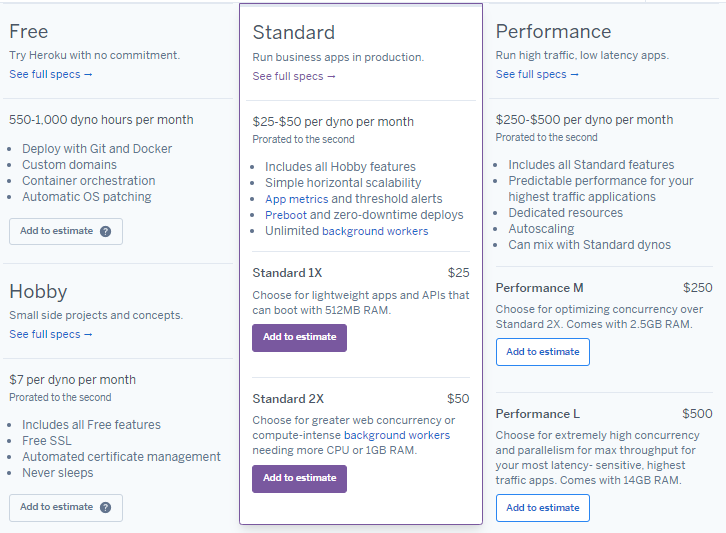
\includegraphics[width=16cm]{imagens/precos-heroku.png}
	\caption{\label{fig:precos-heroku} Preço mensal de aluguel dos \textit{\glspl{dyno}} do Heroku}
	\fonte{\cite{heroku:2021}}
\end{figure}

O custo de hospedagem do \textit{\gls{front-end}} e autenticação variou conforme a quantidade de armazenamento e suporte a acessos simultâneos necessários para atender a quantidade crescente de alunos.

Para a hospedagem do banco de dados será utilizado o Heroku Postgres. Para cada demanda de usuários será utilizado um plano diferente do Heroku Postgres, onde os planos oferecem diferentes quantidades de memória \ac{ram}, armazenamento e acessos simultâneos. Durante a etapa de desenvolvimento será utilizado o plano "Hobby Dev", que é gratuito. Já durante o funcionamento da aplicação será utilizado um plano diferente, visto que cada plano oferta diferentes quantidades de recursos e possuem diferentes valores. Portanto, cada plano será utilizado para atender adequadamente a demanda de usuários.

\begin{itemize}
    \item \textbf{100 alunos}: Standard 0 (4 GB de \ac{ram}, 64 GB de armazenamento e 120 conexões simultâneas por US\$50 mensais);
    \item \textbf{1000 alunos}: Premium 0 (4 GB de \ac{ram}, 64 GB de armazenamento, 120 conexões simultâneas e alta disponibilidade por US\$200 mensais);
    \item \textbf{5000 alunos}: Premium 2 (8 GB de \ac{ram}, 256 GB de armazenamento e 400 conexões simultâneas US\$350 mensais);
    \item \textbf{10000 alunos}: Premium 4 (30.5 GB de \ac{ram}, 1 TB de armazenamento, 500 conexões simultâneas e alta disponibilidade por US\$1200 mensais);
    \item \textbf{50000 alunos}: Premium 7 (244 GB de \ac{ram}, 2 TB de armazenamento, 500 conexões simultâneas e alta disponibilidade por US\$6000 mensais).
\end{itemize}

\section{Entregáveis}
A entrega do projeto é dividida em três fases: a prova de conceito, o mínimo produto viável e o produto pronto.

\subsection{Prova de Conceito (POC)}
A \ac{poc} teve como principal objetivo a validação dos elementos de arquitetura apresentados. Então, para isso, foram desenvolvidas as funcionalidades:
 \begin{itemize}
     \item Cadastro e acesso à aplicação pelo administrador.
 \end{itemize}

\subsection{Mínimo Produto Viável (MVP)}
Para o \ac{mvp}, foram incluídas as funcionalidades:
\begin{itemize}
    \item Perfis do aluno, do professor, do gestor e do administrador;
    \item \ac{crud} de turmas, conquistas, atividades e escolas;
    \item Parametrização de turmas;
    \item Painéis de turmas e de conquistas;
    \item Ranking de alunos.
\end{itemize}

\subsection{Produto Pronto}
Por fim, para o produto pronto, serão consideradas as funcionalidades:

\begin{itemize}
    \item \glspl{dashboard};
    \item Integração com o Google Classroom.
\end{itemize}

Além de tornar o \textit{design} da aplicação responsivo.

\section{Testes}
Nos testes da aplicação, foram desenvolvidos scripts de testes ponta a ponta automatizados utilizando o Cypress. Esta metodologia foi escolhida, pois, com ela, é possível testar todos os elementos da aplicação simulando o ambiente real. 

Nesta seção, serão apresentados os casos de testes implementados bem como os resultados parciais de sua execução.


\subsection{Cadastro de Escolas}
A \autoref{fig:teste-escola} mostra os casos de testes implementados para a entidade Escola da aplicação. O fluxo dos testes se inicia com o acesso na aplicação através de um usuário com o perfil administrador; em seguida é acessado o painel de escolas e nele é realizado o cadastro, alteração de uma escola.

\begin{figure}[htb]
    \centering
	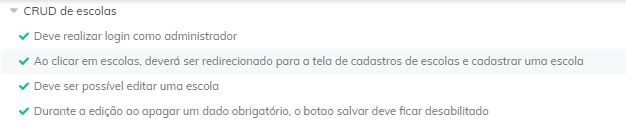
\includegraphics[width=16cm]{imagens/tstEscola.JPG}
	\caption{\label{fig:teste-escola} Casos de testes do cadastro de escolas.}
	\fonte{Os autores}
\end{figure}

\subsection{Cadastro de Usuários}
A \autoref{fig:teste-admin} mostra os casos de testes implementados para usuários com o perfil de administrador. O fluxo desse teste se inicia com o acesso na aplicação através de um usuário com o perfil administrador; em seguida é acessado o painel de usuários e nele é realizado o cadastro, alteração e um usuário

\begin{figure}[htb]
    \centering
	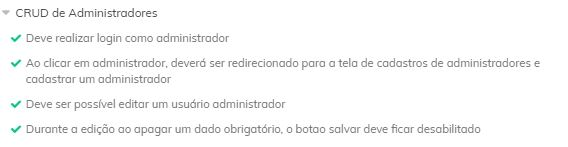
\includegraphics[width=16cm]{imagens/tstAdmin.JPG}
	\caption{\label{fig:teste-admin} Casos de testes do cadastro de administradores.}
	\fonte{Os autores}
\end{figure}

\subsection{Cadastro de Gestores}
A \autoref{fig:teste-gestor} mostra os casos de testes implementados para usuários com o perfil Gestor. O fluxo desse teste se inicia com o acesso na aplicação através de um usuário com o perfil administrador; em seguida é acessado o painel de gestores e nele é realizado o cadastro, alteração de um gestor

\begin{figure}[htb]
    \centering
	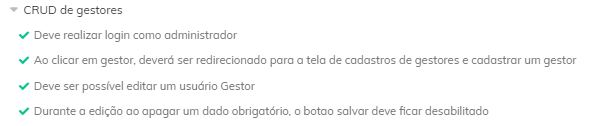
\includegraphics[width=16cm]{imagens/tstGestor.JPG}
	\caption{\label{fig:teste-gestor} Casos de testes do cadastro de gestores.}
	\fonte{Os autores}
\end{figure}

\subsection{Cadastro de Professores}
A \autoref{fig:teste-professor} mostra os casos de testes implementados para usuários com o perfil Professor. O fluxo desse teste se inicia com o acesso na aplicação através de um usuário com o perfil gestor; em seguida é acessado o painel de gestores e nele é realizado o cadastro, alteração de um professor.

\begin{figure}[htb]
    \centering
	
\includegraphics[width=16cm]{imagens/tstProfessor.JPG}
	\caption{\label{fig:teste-professor} Casos de testes do cadastro de professores.}
	\fonte{Os autores}
\end{figure}

\subsection{Cadastro de Alunos}
A \autoref{fig:teste-aluno} mostra os casos de testes implementados para usuários com o perfil Aluno. O fluxo desse teste se inicia com o acesso na aplicação através de um usuário com o perfil gestor; em seguida é acessado o painel de alunos e nele é realizado o cadastro, alteração de um aluno.

\begin{figure}[htb]
    \centering
	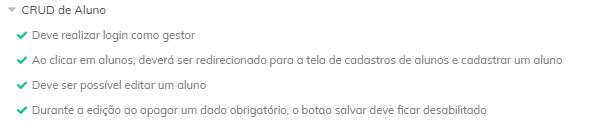
\includegraphics[width=16cm]{imagens/tstAluno.JPG}
	\caption{\label{fig:teste-aluno} Casos de testes do cadastro de alunos.}
	\fonte{Os autores}
\end{figure}

\subsection{Cadastro de Turmas}
A \autoref{fig:teste-turma} mostra os casos de testes implementados para o cadastro de turmas. O fluxo desse teste se inicia com o acesso na aplicação através de um usuário com o perfil gestor; em seguida é acessado o painel de turmas onde é realizado o cadastro, alteração de um aluno.

\begin{figure}[htb]
    \centering
	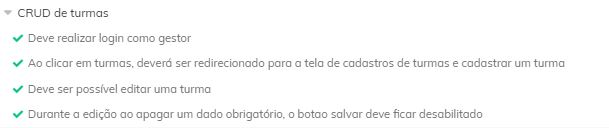
\includegraphics[width=16cm]{imagens/tstTurma.JPG}
	\caption{\label{fig:teste-turma} Casos de testes do cadastro de turmas.}
	\fonte{Os autores}
\end{figure}

\subsection{Cadastro de Conquistas}
A \autoref{fig:teste-conquista} mostra os casos de testes implementados para as conquistas. O fluxo desse teste se inicia com o acesso na aplicação através de um usuário com o perfil de professor e em seguida acessando o painel de  conquistas para realização do cadastro e alteração. 

\begin{figure}[htb]
    \centering
	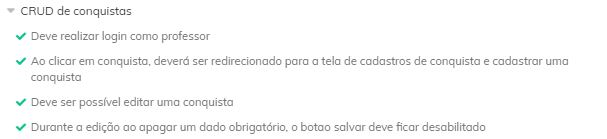
\includegraphics[width=16cm]{imagens/tstConquista.JPG}
	\caption{\label{fig:teste-conquista} Casos de testes do cadastro de conquistas.}
	\fonte{Os autores}
\end{figure}

\subsection{Cobertura de código}

A \autoref{fig:teste-backend} representa o resultado dos testes no \textit{\gls{back-end}}. Com isso, pode-se notar que a cobertura média da aplicação ficou em torno de 40\%, uma nota abaixo do esperado, porém isso aconteceu devido ao curto período de tempo disponível para o desenvolvimento do projeto.
\begin{figure}[htb]
    \centering
	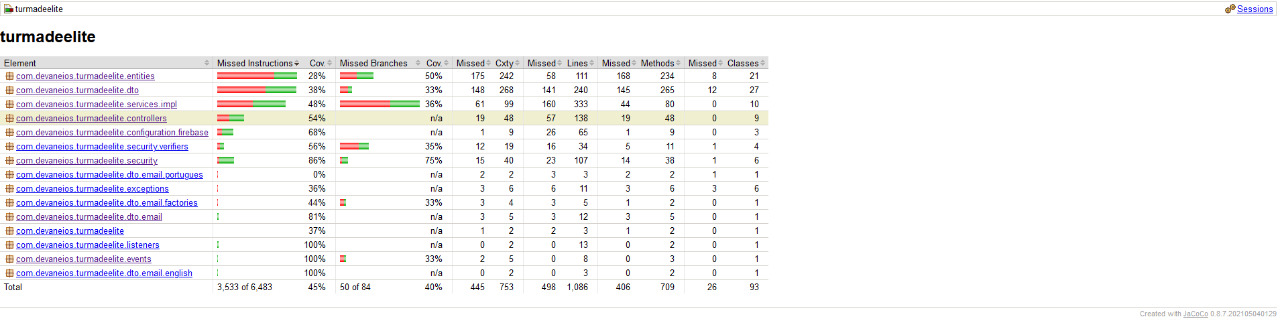
\includegraphics[width=16cm]{imagens/TesteBackend.jpg}
	\caption{\label{fig:teste-backend} Resultado dos testes no back-end.}
	\fonte{Os autores}
\end{figure}

Já no \textit{\gls{front-end}}, após a execução dos testes implementados, foi alcançado o nível de cobertura de código apresentado na \autoref{fig:cobetura}.

\begin{figure}[htb]
    \centering
	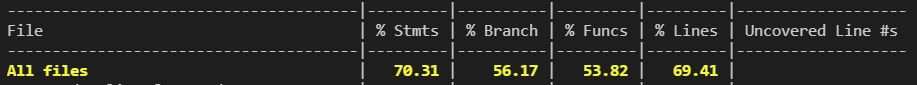
\includegraphics[width=16cm]{imagens/ResultadoTestes.JPG}
	\caption{\label{fig:cobetura} Cobertura de código}
	\fonte{Os autores}
\end{figure}

No geral, os testes no \textit{\gls{front-end}} cobriram 69.41\% das linhas de código, uma  porcentagem não suficiente devido ao tempo curto para o desenvolvimento do projeto.


\section{Escolhas e Descartes}
No início do projeto, foi decidido que para o produto pronto ficaria apenas a integração com o Moodle. Entretanto, para complementá-la, foi necessário ter novas ideias. Uma das ideias que surgiram foi inserir um sistema de boletim na aplicação, entretanto foi logo descartada, pois o Moodle já realiza essa função. Por fim, foi decidido que também ficaria para a próxima entrega os dashboards, além de trazer responsividade para a aplicação. Além disso, ao longo do desenvolvimento, algumas funcionalidades acabaram não fazendo mais sentido ao longo do processo como o envio de e-mail ao gestor para cadastrar dados da sua escola. Ao invés disso, é possível cadastrar seus dados diretamente pelo administrador. 

Outra mudança que também ocorreu foi a utilização do PostgreSQL, ao invés do MySQL, para o armazenamento de dados. Foi uma recomendação do professor orientador Daniel Marques Gomes de Morais, visto que o PostgreSQL é um sistema gerenciador de banco de dados que tem integração com o Heroku, portanto não gera custos adicionais de hospedagem. Com essa mudança, a utilização do Oracle Cloud também foi descartada, visto que ele era usado apenas para hospedar o MySQL e não possuía integração gratuita com o \ac{sgbd}.

Foi alterado também a forma da abordagem da metodologia ágil no projeto. Antes, havia muitas ferramentas, como o Excel e o Notion, que eram atualizadas para seguir o Scrum, mas com as dicas dos professores da banca, foi possível centralizar em uma única ferramenta, o Projects do GitHub, e assim ter uma melhor visualização e fácil alteração dos status das atividades. Além disso, com essa ferramenta também é possível conciliar as tarefas aos seus respectivos códigos, facilitando a identificação do andamento, bem como a geração de métricas do projeto.



\chapter[Considerações Finais]{Considerações Finais}

Com a elaboração da documentação e do desenvolvimento da aplicação até o \ac{mvp}, os integrantes da equipe tiveram a oportunidade de tomar conhecimento da real complexidade que é um desenvolvimento de \textit{\gls{software}}. Para tal, algumas dificuldades ao longo do desenvolvimento ocorreram. 

A primeira e principal dificuldade que todos os integrantes passaram foi o tempo. Como a maioria da equipe já trabalha na área e também houve uma condensação do semestre, isso reduziu a quantidade de horas que poderia ser dedicado ao projeto. Além disso, como havia outras disciplinas com tarefas a serem entregues, com um semestre condensado também, tornava mais difícil conciliar essas entregas com as expectativas do andamento do projeto.

A segunda dificuldade encontrada foi a falta de conhecimento prévio em algumas tecnologias e ferramentas adotadas. Com isso, acabava-se gastando o pouco tempo disponível para buscar saber sobre o assunto. Para tentar minimizar essa dificuldade, nas reuniões semanais, era apresentada a tecnologia em questão, uma visão geral de como funcionava e também \textit{links} para facilitar o entendimento e procura sobre a tecnologia.

A terceira dificuldade foi a utilização de tecnologias obrigatórias pela disciplina. O LaTeX, por exemplo, é uma ferramenta que demandou um grande esforço, pois, mesmo que alguns integrantes da equipe já sabiam utilizar, sempre aparecia uma situação nova para resolver, então era necessário pesquisar e testar diversas soluções para identificar e solucionar o problema. O Overleaf, editor do LaTeX adotado, apresentou algumas instabilidades no decorrer da escrita da documentação da aplicação, ocasionadas por manutenção. Entretanto, tais instabilidades ocorreram raramente e foram resolvidas rapidamente. Além disso, o \gls{svn} também demandou um certo esforço, pois nenhum dos integrantes tinha conhecimento dessa ferramenta.

No caso do gerenciamento do projeto, a principal dificuldade encontrada foi a comunicação entre os integrantes da equipe, afinal era aparente que nem todos estavam satisfeitos e por dentro do andamento do projeto. Então, para minimizar isso, foi criado um documento no \textit{Notion} para que todos colocassem suas atividades do dia, próximos passos e possíveis impedimentos, visando que todos tomassem ciência do andamento do projeto e poder ajudar caso alguém estivesse precisando. Além disso, foi decidido também que a cada duas semanas, todos os integrantes iriam falar o que estavam sentindo em relação ao projeto, para assim todos terem voz e o sentimento de pertencimento dentro da equipe.

Outra dificuldade encontrada no gerenciamento foi lidar com diferentes pessoas, com diferentes formas de pensar e de empenhar-se ao projeto. Foi necessário colocar ao limite o senso crítico para sempre buscar tomar a decisão certa e assim encontrar a melhor saída para possíveis conflitos e desencontros que aconteciam, desde definir os próximos passos para cada integrante até para alinhá-los com as expectativas do desenvolvimento e entregas do projeto.

As dificuldades encontradas ao longo do projeto serviram para o crescimento dos integrantes, bem como a identificação de melhorias para o futuro. Além disso, os conhecimentos adquiridos poderão ser levados não apenas para o desenvolvimento do produto pronto, mas também para o ambiente profissional e pessoal em diversos aspectos.





% ----------------------------------------------------------
% Finaliza a parte no bookmark do PDF
% para que se inicie o bookmark na raiz
% e adiciona espaço de parte no Sumário
% ----------------------------------------------------------
\phantompart

% ----------------------------------------------------------
% Referências bibliográficas
% ----------------------------------------------------------
% quando não esta utilizando biblatex tem que carregar as referencias aqui
\IfPackageLoaded{biblatex}{}{%
\bibliography{referencias,exemplos/abntex2-doc-abnt-6023}
}

% ----------------------------------------------------------
% Glossário
% ----------------------------------------------------------
%

 \ifdef{\printnoidxglossary}{
     \addcontentsline{toc}{chapter}{GLOSSÁRIO}
     \printnoidxglossary[style=glossario]
}{}
% ----------------------------------------------------------
% Apêndices
% Documentos gerados pelo próprio autor
% ----------------------------------------------------------

% ---
% Inicia os apêndices
% ---
\begin{apendicesenv}

% Imprime uma página indicando o início dos apêndices
\partapendices
% ----------------------------------------------------------
\chapter{Proposta Inicial}
% ----------------------------------------------------------
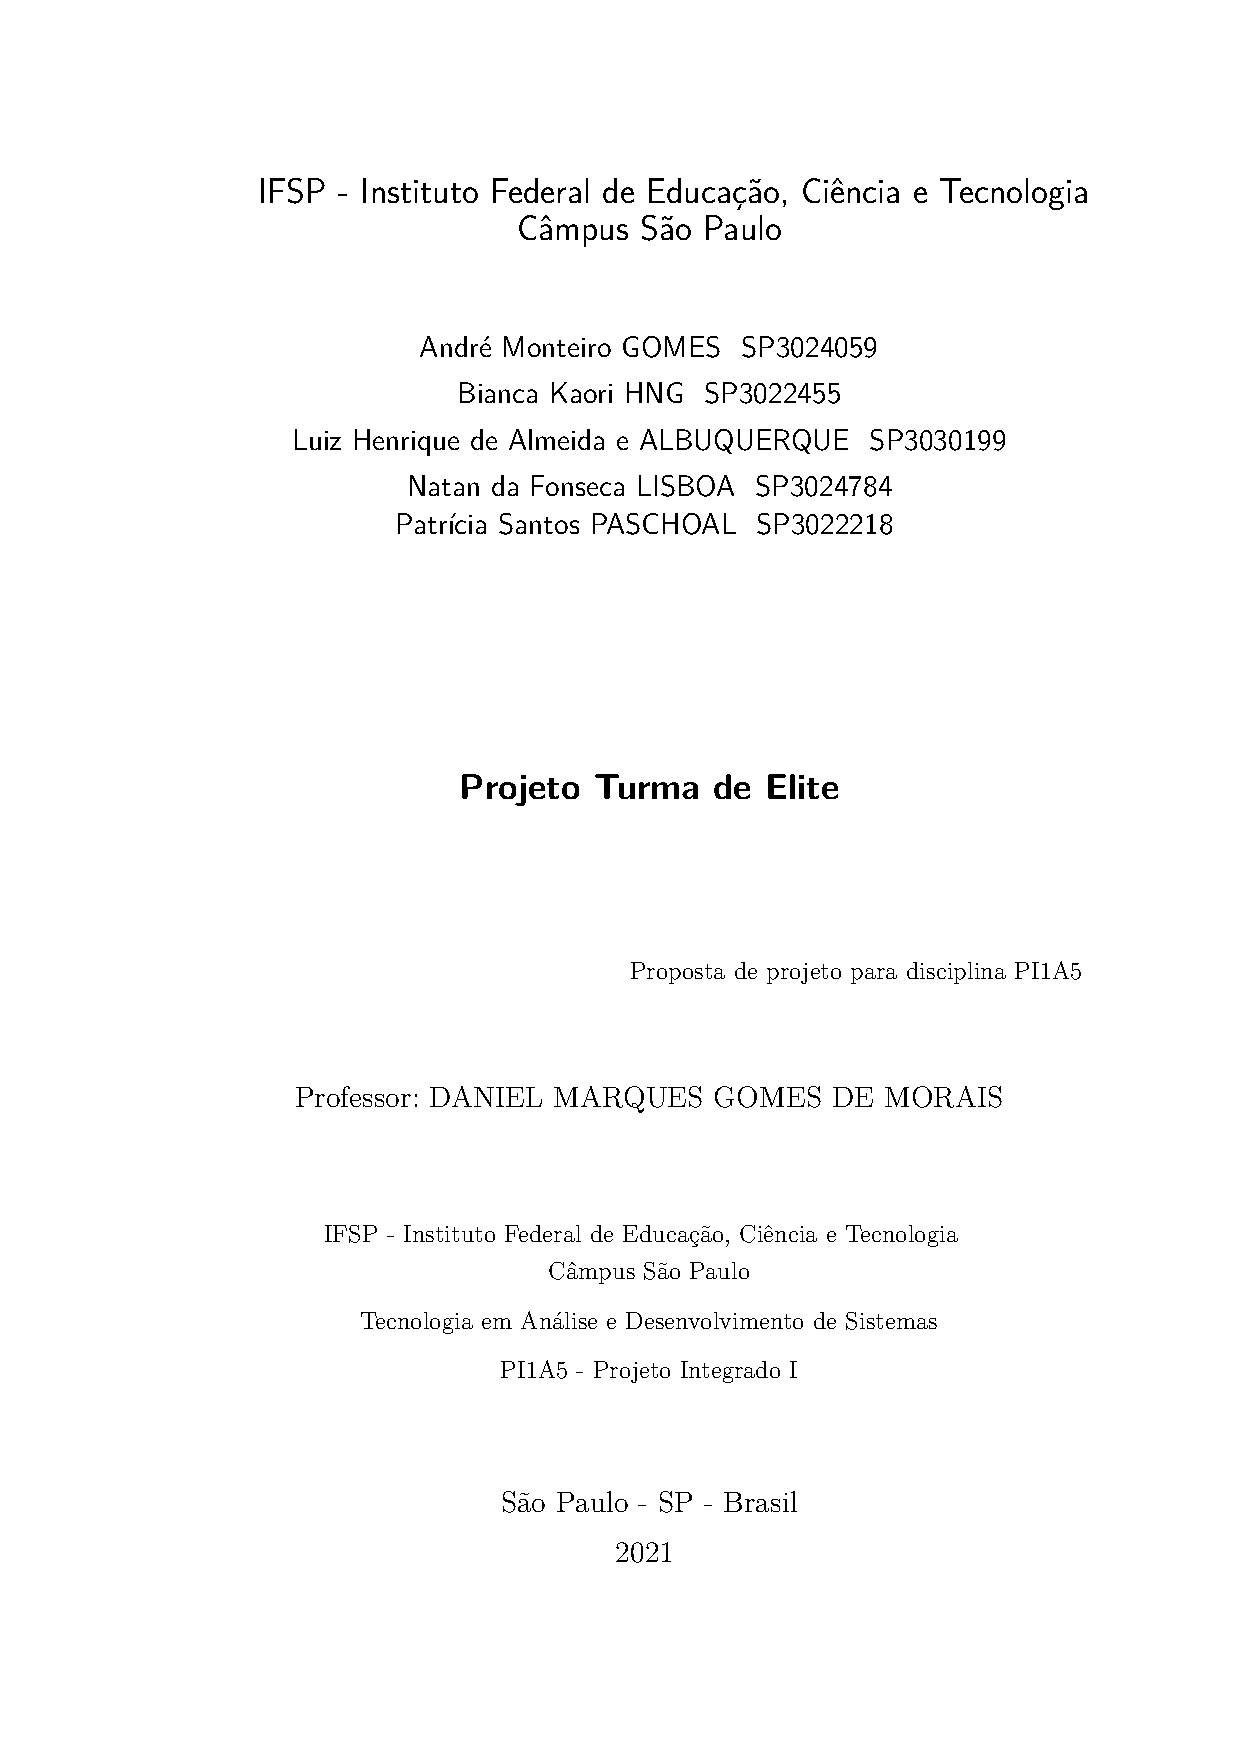
\includepdf[pages=-]{EntregaFinal/PropostaInicial.pdf}

% ----------------------------------------------------------
\chapter{Sprints}
\label{sprints-atividades}
% ----------------------------------------------------------

Esta seção apresenta as atividades planejadas em cada \gls{sprint}.


\section{Sprint 1 - 10/05/2021 a 25/05/2021}

O \autoref{quadro-sprint1} mostra a divisão de tarefas da equipe ao longo da sprint.

\begin{quadro}[htb]
\centering
\ABNTEXfontereduzida
\caption{Sprint 1 - 10/05/2021 a 25/05/2021}
\label{quadro-sprint1}
\begin{tabular}{|l|c|}
\hline
{\thead{Atividade}} & \thead{Responsável}  \\ \hline
    Concepção do Projeto & André     \\ \hline 
    Concepção do Projeto & Bianca     \\ \hline
    Concepção do Projeto & Luiz      \\ \hline
    Concepção do Projeto & Natan   \\ \hline
    Concepção do Projeto & Patrícia    \\ \hline
    Pesquisa sobre outras aplicações  & André     \\ \hline  
    \multicolumn{2}{|c|}{Proposta Inicial} \\ \hline
    Justificativa                     & Natan    \\ \hline
    Objetivo                          & Luiz     \\ \hline
    Escopo                            & Patrícia \\ \hline
    Integrações                       & André     \\ \hline   
    Tecnologia e Infraestrutura       & André     \\   \hline
    Tecnologia e Infraestrutura       & Patrícia  \\ \hline
    Parcerias e Viabilidade Comercial & Patrícia \\ \hline 
    Revisão da Documentação           & Bianca   \\ \hline  
    Apresentação                      & Bianca  \\ \hline 
    \multicolumn{2}{|c|}{Blog} \\ \hline
    Postagem - Semana 01      & Bianca  \\ \hline
    Postagem - Semana 02      & Bianca     \\ \hline
\end{tabular}
\fonte{Os autores}
\end{quadro}
\FloatBarrier

\section{Sprint 2 - 25/05/2021 a 08/06/2021}
O \autoref{quadro-sprint2} demonstra as atividades concluídas na Sprint 2.
\begin{quadro}[htb]
\centering
\ABNTEXfontereduzida
\caption{Sprint 2 - 25/05/2021 a 08/06/2021}
\label{quadro-sprint2}
\begin{tabular}{|l|c|}
\hline
{\thead{Atividade}} & \thead{Responsável}  \\ \hline  
    \multicolumn{2}{|c|}{Proposta Inicial} \\ \hline
    Ajustes - Justificativa           & Patrícia     \\ \hline
    Ajustes - Objetivo                & Patrícia     \\ \hline
    Detalhamento do Escopo            & Patrícia \\ \hline
    Ajustes - Escopo                  & Patrícia    \\ \hline   
    Ajustes - Análise Comparativa       & Natan      \\   \hline
    Ajustes - Análise Comparativa       & Bianca \\ \hline
    Evoluções Previstas  & Patrícia \\ \hline 
    Ajustes - Integrações          & Natan \\ \hline  
    Ajustes - Tecnologias            & Natan   \\ \hline 
    Ajustes - Tecnologias                   & Luiz  \\ \hline 
    Monetização    & Bianca  \\ \hline 
    Monetização    & Natan  \\ \hline 
    Suporte nos Ajustes  & André   \\ \hline 
    Formatação da Documentação & Patrícia  \\ \hline 
    Formatação da Documentação & Luiz   \\ \hline 
    Revisão da Documentação & Bianca   \\ \hline 
    Ajustes - Apresentação & Bianca  \\ \hline 
    
    \multicolumn{2}{|c|}{Desenho da Aplicação} \\ \hline
    Introdução  & Natan  \\ \hline 
    Revisão Bibliográfica  & Natan  \\ \hline 
    Arquitetura da Solução  & Patrícia   \\ \hline 
    Escopo  & Patrícia  \\ \hline 
    Escopo  & Bianca   \\ \hline 
    Viabilidade Financeira  & Natan  \\ \hline 
    Escalabilidade  & Patrícia  \\ \hline 
    Segurança  & Luiz  \\ \hline 
    Tecnologias  & Luiz \\ \hline 
    Manutenibilidade da aplicação  & Patrícia   \\ \hline 
    Metodologias  & Bianca  \\ \hline 
    Revisão da Documentação  & Luiz \\ \hline 
    
    \multicolumn{2}{|c|}{Desenvolvimento do Back-End} \\ \hline
    Criar repositório no github & André  \\ \hline 
    Preparação do ambiente & André  \\ \hline 
    Configuração do banco de dados em produção & André  \\ \hline 
    Autenticação pelo firebase & André  \\ \hline 
    Fluxo de primeiro acesso & André  \\ \hline 
    Teste de primeiro acesso (integração) & André  \\ \hline 
    
    \multicolumn{2}{|c|}{Desenvolvimento do Front-End} \\ \hline
    Criar repositório no github & André  \\ \hline 
    Criar tela de login & André  \\ \hline 
    Criar tela de novo acesso & André \\ \hline 
    
    \multicolumn{2}{|c|}{Blog} \\ \hline
    Postagem - Semana 03      & Bianca      \\ \hline
    Postagem - Semana 04      & Bianca      \\ \hline
    
    \multicolumn{2}{|c|}{Vídeo} \\ \hline
    Gravar o vídeo da proposta inicial & Natan  \\ \hline 
\end{tabular}
\fonte{Os autores}
\end{quadro}
\FloatBarrier

\section{Sprint 3 - 08/06/2021 a 22/06/2021}
O \autoref{quadro-sprint3} representa as atividades realizadas ao longo da sprint.
\begin{quadro}[htb]
\centering
\ABNTEXfontereduzida
\caption{Sprint 3 - 08/06/2021 a 22/06/2021}
\label{quadro-sprint3}
\begin{tabular}{|l|c|}
\hline
{\thead{Atividade}} & \thead{Responsável}  \\ \hline
    \multicolumn{2}{|c|}{Desenho da Aplicação} \\ \hline
    Ajustes - Lista de Siglas           & Natan     \\ \hline
    Ajustes - Introdução                          & Natan \\ \hline
    Ajustes - Arquitetura de Solução              & Patrícia \\ \hline
    Ajustes - Escopo                       & Bianca     \\ \hline   
    Ajustes - Viabilidade Financeira       & Natan   \\   \hline
    Ajustes - Metodologias       & Bianca \\ \hline
    Ajustes - Product Backlog & Patrícia  \\ \hline 
    Revisão da Documentação           & Natan \\ \hline  
    Configuração do LaTeX diff     & Natan   \\ \hline 
    Apresentação 		 & Bianca  \\ \hline
    
     \multicolumn{2}{|c|}{Histórias de Usuário} \\ \hline
     Administrador & André  \\ \hline
     Gestor & Luiz   \\ \hline
     Professor & Bianca \\ \hline
     Aluno & Patrícia  \\ \hline
     Criar mais histórias de usuário & Patrícia  \\ \hline
    
    \multicolumn{2}{|c|}{Desenvolvimento do Back-End} \\ \hline
    Autenticação e Autorização & André \\ \hline 
    Cadastro e Visualização do Administrador & André  \\ \hline 
    Envio de e-mail do primeiro acesso & André \\ \hline 
    
    \multicolumn{2}{|c|}{Desenvolvimento do Front-End} \\ \hline
    Elaboração de Protótipos de baixa fidelidade & André \\ \hline 
    Elaboração de Protótipos de baixa fidelidade & Luiz  \\ \hline 
    
    \multicolumn{2}{|c|}{Blog} \\ \hline
    Postagem - Semana 05      & Bianca    \\ \hline
    Postagem - Semana 06      & Bianca   \\ \hline
    
    \multicolumn{2}{|c|}{Vídeo} \\ \hline
    Gource & Natan \\ \hline
    
\end{tabular}
\fonte{Os autores}
\end{quadro}
\FloatBarrier

\section{Sprint 4 - 22/06/2021 a 06/07/2021}
 A Sprint 4 foi principalmente dedicada às entregas da POC e ajustes no desenho da aplicação. O \autoref{quadro-sprint4} representa as atividades realizadas ao longo da sprint.
 
\begin{quadro}[htb]
\centering
\ABNTEXfontereduzida
\caption{Sprint 4 - 22/06/2021 a 06/07/2021}
\label{quadro-sprint4}
\begin{tabular}{|l|c|}
\hline
{\thead{Atividade}} & \thead{Responsável}  \\ \hline
    \multicolumn{2}{|c|}{Desenho da Aplicação} \\ \hline
    Tag SVN           & Natan   \\ \hline
    \multicolumn{2}{|c|}{Prova de Conceito} \\ \hline
    Ajustes no código                     & André     \\ \hline
    Subir no SVN                & Bianca  \\ \hline
    Apresentação                & André \\ \hline
    Relatório                       & André     \\ \hline   
    Formatação LaTeX       & Natan      \\   \hline
    Vídeo       & Natan  \\ \hline
    Desenhar arquitetura & Patrícia   \\ \hline 
    Tags SVN           & Natan   \\ \hline  
    
    \multicolumn{2}{|c|}{Desenvolvimento do Back-End} \\ \hline
    Criar listagem e paginação de administradores cadastrados & André    \\ \hline   
    Arrumar fluxo de login e primeiro acesso & André    \\ \hline 
    Criar cadastro de escolas & André    \\ \hline   
    Aumentar cobertura de testes & André    \\ \hline  
    Exclusão de administradores & Patrícia   \\ \hline 
    
    \multicolumn{2}{|c|}{Desenvolvimento do Front-End} \\ \hline
    Criar tela de cadastro de escolas & André   \\ \hline 
    Elaboração de Protótipos de alta fidelidade & Patrícia   \\ \hline 
    Elaboração de Protótipos de alta fidelidade & Luiz  \\ \hline 
    
    \multicolumn{2}{|c|}{Blog} \\ \hline
    Ajustes no conteúdo  & Bianca      \\ \hline
    Postagem - Semana 07      & Bianca     \\ \hline
    Postagem - Semana 08      & Bianca      \\ \hline
    
    \multicolumn{2}{|c|}{Vídeo} \\ \hline
    Gource (POC) & Natan   \\ \hline 
    Gravação do vídeo (Desenho da Aplicação) & Bianca     \\ \hline
    Gravação do vídeo (Desenho da Aplicação) & Luiz   \\ \hline
    Gravação do vídeo (Desenho da Aplicação) & Natan   \\ \hline
    Gravação do vídeo (Desenho da Aplicação) & Patrícia    \\ \hline
    
    \multicolumn{2}{|c|}{LaTeX} \\ \hline
    Adequação dos arquivos em LaTeX & Natan   \\ \hline 
    Subir no SVN & Natan   \\ \hline
    
\end{tabular}
\fonte{Os autores}
\end{quadro}
\FloatBarrier

\section{Sprint 5 - 06/07/2021 a 20/07/2021}
Com as datas de entrega da documentação final e da apresentação próximas, dedicou-se um maior tempo ao desenvolvimento do projeto. O \autoref{quadro-sprint5} representa as atividades realizadas ao longo da sprint.
\begin{quadro}[htb]
\centering
\ABNTEXfontereduzida
\caption{Sprint 5 - 06/07/2021 a 20/07/2021}
\label{quadro-sprint5}
\begin{tabular}{|l|c|}
\hline
{\thead{Atividade}} & \thead{Responsável} \\ \hline
    \multicolumn{2}{|c|}{Documentação Final} \\ \hline
    Ajustes na estrutura do documento & Bianca \\ \hline
    Ajustes - Revisão de Literatura & Bianca   \\ \hline 
    Atividades das sprints       & Bianca  \\ \hline
    Postagens do blog  & Bianca  \\ \hline
    Métricas do projeto  & Bianca    \\ \hline   
    Proposta Inicial  & Bianca    \\ \hline  
    QR Codes       & Luiz    \\   \hline
    QR Codes       & Natan      \\   \hline
    Escolhas e Descartes       & Luiz  \\ \hline
    Escolhas e Descartes & Bianca   \\ \hline 
    Ajustes - Escopo & Bianca   \\ \hline 
    Modelagem de Dados & Natan   \\ \hline 
    Testes Front-end & Patricia  \\ \hline 
    Testes Back-end & Bianca   \\ \hline 
    Entregáveis & Bianca  \\ \hline 
    Ajustes - Segurança & Bianca  \\ \hline 
    Considerações Finais   & Bianca    \\ \hline  
    
    \multicolumn{2}{|c|}{Desenvolvimento do Back-End} \\ \hline
    Cadastro de conquista & André    \\ \hline  
    Entrega de conquista & André    \\ \hline 
    CRUD de gestores & André    \\ \hline  
    CRUD de alunos & André    \\ \hline  
    CRUD de professores & André   \\ \hline 
    Endpoint cadastro de turma & André    \\ \hline
    Endpoint cadastro de atividades & André     \\ \hline  
    Busca dinâmica de escolas & Natan   \\ \hline 
    Busca dinâmica de administradores & Natan   \\ \hline 
    Busca dinâmica de gestores & Natan   \\ \hline 
    Busca dinâmica de professores & Natan   \\ \hline
    Criação dos loaders & Gustavo   \\ \hline 
    Traduções dos placeholders & Gustavo \\ \hline 
    Tratamento de erros nos formulários & Gustavo  \\ \hline 
    Aumentar cobertura de testes & André      \\ \hline 
    
    \multicolumn{2}{|c|}{Desenvolvimento do Front-End} \\ \hline
    Configuração do Cypress & André    \\ \hline 
    Tela do cadastro de turmas & André  \\ \hline 
    Tela do cadastro de atividades & André   \\ \hline
    Listagem de turmas & André \\ \hline 
    Visão do professor & André  \\ \hline 
    Tela de criação de professor & Gustavo   \\ \hline 
    Testes de Escolas & Patricia \\ \hline 
    Testes de Administradores & Patricia  \\ \hline 
    Testes de Gestores & Patricia  \\ \hline 
    Testes de Professores & Patricia  \\ \hline 
    Configurar relatórios de testes & Patricia  \\ \hline 
    Estilização de telas & Patricia \\ \hline 
    
    \multicolumn{2}{|c|}{Blog} \\ \hline
    Postagem - Semana 09      & Bianca      \\ \hline
    Postagem - Semana 10      & Bianca   \\ \hline
    
    \multicolumn{2}{|c|}{Vídeo} \\ \hline
    Gource (POC) & Natan  \\ \hline 
    
    
\end{tabular}
\fonte{Os autores}
\end{quadro}
\FloatBarrier

\section{Sprint 6 - 20/07/2021 a 03/08/2021}
No período da Sprint 6, iniciou-se as provas das outras disciplinas, por conta disso não foi possível dedicar-se tanto ao projeto. O \autoref{quadro-sprint6} representa as atividades realizadas ao longo da sprint.

\begin{quadro}[htb]
\centering
\ABNTEXfontereduzida
\caption{Sprint 6 - 20/07/2021 a 03/08/2021}
\label{quadro-sprint6}
\begin{tabular}{|l|c|}
\hline
{\thead{Atividade}} & \thead{Responsável}  \\ \hline
    \multicolumn{2}{|c|}{Documentação Final} \\ \hline
    Ajustes gerais no documento                & Bianca  \\ \hline
    Ajustes gerais no documento                & Luiz \\ \hline
    Apresentação final               & Bianca  \\ \hline
    
    \multicolumn{2}{|c|}{Desenvolvimento do Back-End} \\ \hline
    Listagem de Atividades & André    \\ \hline  
    Envio de anexos & André    \\ \hline 
    Entrega de Atividades & André    \\ \hline   
    Encerramento de turmas & André    \\ \hline  
    
    \multicolumn{2}{|c|}{Desenvolvimento do Front-End} \\ \hline
    Validação dos formulários de atividades & Gustavo   \\ \hline 
    Ajustes nas validações dos campos & Gustavo   \\ \hline 
    Aprofundamento do entendimento do Cypress & Patrícia   \\ \hline 
    Aumento da cobertura de testes & Patrícia   \\ \hline 
    
    \multicolumn{2}{|c|}{Blog} \\ \hline
    Postagem - Semana 11      & Bianca     \\ \hline
    Postagem - Semana 12      & Bianca      \\ \hline
    
    \multicolumn{2}{|c|}{Vídeo} \\ \hline
    Gource (MVP) & Natan   \\ \hline 
    
    \multicolumn{2}{|c|}{LaTeX} \\ \hline
    Subir no SVN & Luiz   \\ \hline
    Suporte na subida para o SVN & Natan   \\ \hline
    
\end{tabular}
\fonte{Os autores}
\end{quadro}
\FloatBarrier

\section{Sprint 7 - 03/08/2021 a 17/08/2021}
Como um dos pontos levantados pelos professores da banca foi que a equipe não estava seguindo a metodologia ágil da forma correta, foi necessária uma reestruturação na metodologia adotada. Para isso, passou-se a fazer o Sprint Backlog no kanban do GitHub. Dessa forma, é possível unificar as tarefas feitas com os respectivos códigos, além de melhorar a criação de métricas para o projeto. A \autoref{sprint7} demonstra o kanban criado para o Sprint Backlog.

\begin{figure}[htb]
    \centering
	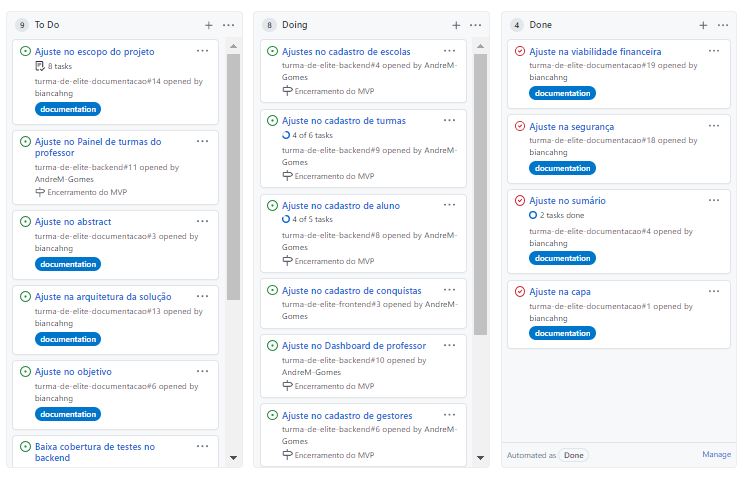
\includegraphics[width=16cm]{imagens/sprint7.png}
	\caption{\label{sprint7} Sprint Backlog da sprint 7}
	\fonte{Os autores}
\end{figure}
\FloatBarrier

% ----------------------------------------------------------
\chapter{Publicações do Blog}
% ----------------------------------------------------------

Ao longo do desenvolvimento do projeto, foram feitas postagens semanais no blog a respeito das atividades exercidas por cada integrante, sobre as reuniões realizadas e decisões tomadas pela equipe.

\section{Resumo de Atividades - Semana 1}

Esse blog tem como objetivo mostrar um acompanhamento semanal do projeto que estamos desenvolvendo para a disciplina de Projeto Integrado I (PI1A5).

Na primeira semana, definimos os integrantes da equipe:

\begin{itemize}
\item André Monteiro Gomes;
\item Bianca Kaori Hng;
\item Luiz Henrique de Almeida e Albuquerque;
\item Natan da Fonseca Lisboa;
\item Patricia Santos Paschoal.
\end{itemize}

E como ideia principal foi decidido que seria algo voltado para a educação, devido à proximidade de alguns dos integrantes com a área e também devido ao fato de já houver alguns esboços de ideias relacionados a isso pelos próprios integrantes. 

A metodologia de gestão adotada foi o Scrum e a gerente do projeto escolhida fui eu, Bianca.

Então, a Patrícia começou a elicitar possíveis requisitos para a aplicação e o André, possíveis tecnologias a serem usadas.

O nome escolhido para a equipe foi "DevAneios", sugerido pelo Natan e, para o nome do projeto, foi escolhido "Turma de Elite", sugerido pelo Luiz. E eu, Bianca, criei o canal do YouTube e o Blog para o projeto.

Fizemos uma reunião com todos os integrantes e, assim, ficou decidido que o projeto aplicaria conceitos de gamificação para a execução de atividades, com o objetivo de incentivar os alunos a desenvolverem as tarefas.


\section{Resumo de Atividades - Semana 2}
Apresentamos a ideia do projeto para o professor e esta foi aceita por ele com a orientação de aprofundá-la para a apresentação da próxima semana. 

Então, a segunda semana foi dedicada ao amadurecimento da ideia e a elaboração do documento e a apresentação da proposta inicial para a turma. 

Nos reunimos duas vezes ao longo da semana: a primeira para amadurecer a ideia do projeto, tanto as funcionalidades que o sistema terá, quanto as tecnologias que serão utilizadas, e também para definir os próximos passos de cada um; e a segunda reunião foi para o alinhamento da equipe para a apresentação da proposta inicial.

Assim, ficou decidido que a aplicação teria um módulo para as atividades, painel de conquistas, ranking dos alunos por liga e \glspl{dashboard} para acompanhamento.
Segue abaixo as atividades de cada integrante:

\begin{itemize}
\item André: trouxe as ideias para o aperfeiçoamento do projeto, pesquisa sobre outras aplicações e fez a elaboração da documentação (integração e tecnologias utilizadas);
\item Bianca: fez a elaboração da apresentação, revisão da documentação e ficou responsável pelas postagens semanais no blog;
\item Luiz: fez a elaboração da documentação (objetivo);
\item Natan: fez a elaboração (justificativa) e revisão da documentação, e a sua conversão para LaTeX;
\item Patricia: fez a elaboração da documentação (escopo, parcerias e tecnologias utilizadas) e mapeamento das funcionalidades da aplicação.
\end{itemize}

\section{Resumo de Atividades - Semana 3}
Apresentamos a proposta inicial para o professor e aos demais alunos da turma. E com o \gls{feedback} do professor, nos reunimos para estabelecer os principais pontos apontados por ele e dividimos as tarefas para cada um.

Para facilitar a comunicação entre os integrantes da equipe e ver o andamento do projeto, foi decidido que uma vez por semana a equipe se reuniria para os \glspl{checkpoint} semanais. O dia escolhido foi terça-feira às 19h30 pois era o melhor dia e horário para todos os integrantes. 

Então, a terceira semana foi dedicada aos ajustes da apresentação e da documentação da proposta inicial e também ao início do desenvolvimento da aplicação.

Segue abaixo as atividades de cada integrante:

\begin{itemize}
\item André: focou na parte de desenvolvimento da aplicação, então criou uma organização no \gls{github}, fez a implementação da autenticação, preparação do \ac{ci} e preparação dos ambientes para receber a aplicação, e também prestou suporte para a documentação;
\item Bianca: fez os ajustes da documentação (análise comparativa e monetização) e da apresentação, bem como a revisão da documentação da proposta inicial, além da preparação de arquivos para a gestão do projeto e criação do equipe.yaml;
\item Luiz: fez os ajustes da documentação (tecnologias) e auxiliou na formatação da documentação da proposta inicial;
\item Natan: fez os ajustes da documentação (análise comparativa, integrações, tecnologias e monetização), auxiliou na sua formatação e fez a gravação e postagem do vídeo de apresentação da proposta inicial;
\item Patrícia: fez os ajustes (evoluções previstas), o melhoramento (justificativa e objetivo) e a formatação da documentação da proposta inicial, bem como o detalhamento do escopo.
\end{itemize}

\section{Resumo de Atividades - Semana 4}
Tivemos uma reunião para acompanhamento do projeto e eventuais dúvidas com o professor e também tivemos uma reunião de \gls{checkpoint} e definição de próximos passos para o projeto, no qual foi definido que focaríamos no desenho da aplicação e no desenvolvimento inicial dos testes.

Então, a quarta semana foi dedicada à elaboração do desenho e início da implementação dos testes. 

Segue abaixo as atividades de cada integrante:

\begin{itemize}
\item André: fez a implementação de autenticação/autorização com Firebase Authentication, criação de \gls{setup} para teste de integração e a integração com ferramentas de análise estática (Deepsource e Eslint);
\item Bianca: fez a elaboração do desenho da aplicação, fazendo a parte de metodologias e escopo, além da revisão do desenho;
\item Luiz: fez a elaboração do desenho da aplicação, fazendo a parte de segurança e tecnologias, e revisão da documentação ;
\item Natan: fez a elaboração do desenho da aplicação, fazendo a parte da introdução, revisão bibliográfica e viabilidade financeira;
\item Patricia: fez a elaboração do desenho da aplicação, fazendo a parte da arquitetura de solução, escopo, escalabilidade e manutenibilidade da aplicação.
\end{itemize}

\section{Resumo de Atividades - Semana 5}
Na quinta semana, tivemos uma reunião de acompanhamento com o professor e mostramos o desenho de aplicação a ele. E, ao longo dessa reunião, ele apontou alguns pontos de melhoria.

Decidimos levar mais a sério a metodologia adotada, então na reunião semanal da equipe, tratamos de marcar todas as entregas que tivemos na \gls{sprint} (Sprint Review) e o que podia ser melhorado (Sprint Retrospective). Um dos pontos levantados para melhoria foi a falta de uma definição clara do projeto. Então, como plano de ação, decidimos levantar as histórias de usuário, para a partir disso sabermos se todos estavam alinhados com as funcionalidades do projeto. 

Dividimos as histórias por tipos de usuários para cada um e, depois de escritas, nos reunimos mais uma vez para discutirmos o que fazia parte do escopo e o que não.

Em paralelo, foram configurados os vídeos do Gource e com isso mostrou-se necessário uma logo para o projeto.

Além disso, foram feitos os ajustes no desenho do projeto, a preparação da apresentação dele e a preparação para a \ac{poc}.

Segue abaixo as atividades de cada integrante:

\begin{itemize}
\item André: configurou o Firebase em produção, implementou testes integrados com Firebase Emulator e escreveu as histórias de usuário do administrador;
\item Bianca: escreveu as histórias de usuário do professor, fez os ajustes no desenho da aplicação (metodologia e modelagem da aplicação) e fez a elaboração da apresentação do desenho;
\item Luiz: fez a elaboração de vários logos para ser escolhida pela equipe, melhorou aquela que foi mais votada e escreveu as histórias de usuário do gestor;
\item Natan: colocou a lista de siglas e o glossário no desenho da aplicação, revisou e criou o latexdiff nele, alterou a parte da introdução e da viabilidade financeira e configurou os vídeos do Gource;
\item Patricia: escreveu as histórias de usuário do aluno e reescreveu a escalabilidade, arquitetura da solução, padrão do projeto e \gls{coding-convention} do desenho da aplicação.
\end{itemize}

\section{Resumo de Atividades - Semana 6}
Assistimos as apresentações do desenho do projeto das outras equipes e, com os \glspl{feedback} do professor para eles, anotamos o que precisaria alterar no nosso desenho. Então, a sexta semana teve como principal foco as mudanças no desenho da aplicação, principalmente na modelagem do projeto. E também tratamos do relatório de avaliação das outras equipes.

Além disso, nos reunimos para o \gls{checkpoint} semanal e nele decidimos fazer um acompanhamento diário das atividades, visto que, desse modo, conseguiríamos ter uma melhor visualização das atividades ao longo da semana. Por isso, criamos uma página no Notion para fazermos a nossa \textit{Daily}.

E, na parte de códigos, focamos no desenvolvimento da \ac{poc}, corremos atrás para validar se todos os pontos dela foram cumpridos e também lidamos com o desenvolvimento dos testes e questões de segurança.

Segue abaixo as atividades de cada integrante:

\begin{itemize}
\item André: desenvolveu a \ac{poc}, iniciou os protótipos de baixa fidelidade, fez os testes de integração para autenticação e melhorou a nota no securityheaders.com;
\item Bianca: criou a página no Notion, fez o relatório da avaliação das outras equipes (ConsacreTADS) e alterou o desenho do projeto (metodologia e escopo) e a apresentação;
\item Luiz: iniciou os protótipos de alta fidelidade
Natan: fez a \gls{checklist} das tarefas da \ac{poc} e da aplicação, fez o relatório de avaliação das outras equipes (AcadTech) e ajustou a formatação do desenho da aplicação;
\item Patricia: criou mais histórias de usuários, fez o mapeamento delas por funcionalidade e ordem de importância, gerando assim o \gls{product-backlog} mais atualizado.
\end{itemize}

\section{Resumo de Atividades - Semana 7}
Na sétima semana, apresentamos o desenho da aplicação para o professor e para os demais alunos da turma. E anotamos o feedback do professor, sob a orientação dele de manter o desenho da aplicação como estava no \ac{svn} e melhorá-lo para a documentação final.

Então, no nosso checkpoint semanal, decidimos focar na \ac{poc}, nos protótipos da aplicação e nas entregas gerais do projeto para a disciplina. E também gravamos vídeos para postar no YouTube.

Segue abaixo as atividades de cada integrante:

\begin{itemize}
\item André: criou a listagem e a paginação de administradores cadastrados, consertou o fluxo de login e primeiro acesso, subiu a versão de \gls{release} para a apresentação da \ac{poc} e fez o relatório e apresentação dela;
\item Bianca: gravou o vídeo da apresentação do desenho do projeto, começou a alterar o modelo lógico da aplicação, alterou o equipe.yaml para colocar as \ac{url}s que faltavam e fez a revisão do relatório da \ac{poc};
\item Luiz: gravou o vídeo da apresentação do desenho do projeto e começou a elaboração dos protótipos de alta fidelidade;
\item Natan: gravou o vídeo da apresentação do desenho do projeto e da prova de conceito, fez sua edição e postagem no YouTube, gerou o vídeo do Gource e adicionou as tags no \ac{svn} até o desenho do projeto ;
\item Patricia: fez os protótipos a nível \gls{wireframe} da visão do aluno, gravou o vídeo da apresentação do desenho do projeto, fez a prototipação de alta fidelidade das telas de login e visão do aluno e fez a modelagem de diagramas para a \ac{poc}.
\end{itemize}

\section{Resumo de Atividades - Semana 8}
Na oitava semana apresentamos a prova de conceito para o professor e para os demais alunos da turma.

Ao longo da semana, nos reunimos para o \gls{checkpoint} semanal e nele foi decidido que toda a equipe direcionaria seus esforços para o desenvolvimento da aplicação.

Então, tivemos uma reunião de alinhamento de código, na qual foi explicado sua estrutura e como configurar na máquina local, bem como a definição dos próximos passos.

Além disso, foram feitos ajustes gerais na documentação e no \ac{svn}.

Segue abaixo as atividades de cada integrante:

\begin{itemize}
\item André: aumentou a cobertura de testes do sistema, conduziu a reunião de alinhamento do código e criou cadastro de escolas no \glspl{back-end};
\item Bianca: iniciou a escrita da documentação final, configurou o projeto para rodar em máquina local e fez edição de escolas;
\item Luiz: fez a prototipação de alta fidelidade da visão do professor;
\item Natan: fez os ajustes da estrutura de arquivos da documentação LaTeX no Overleaf, atualizou as \textit{tags} no repositório e fez o relatório de avaliação da apresentação da prova de conceito das outras equipes; 
\item Patricia: fez a prototipação de alta fidelidade da visão do gestor, configurou o projeto para rodar em máquina local e criou a exclusão de administradores no \glspl{back-end}.
\end{itemize}

\section{Resumo de Atividades - Semana 9}
Na nona semana ficamos sabendo que um dos grupos da sala seria desfeito devido ao fato de que duas integrantes trancariam a disciplina. Então, os outros três integrantes foram alocados nas outras equipes e assim o Gustavo entrou para a nossa equipe :)

Desse modo, a semana foi dedicada em passar as principais informações a respeito do projeto ao novo integrante, além do desenvolvimento da aplicação e da documentação final.

A nossa reunião semanal foi voltada a uma retrospectiva do projeto, na qual todos os integrantes falaram o que estavam achando em relação ao projeto, o que estavam gostando e o que não estavam gostando, de modo a saber se todos os integrantes estavam alinhados e satisfeitos com o desenvolvimento do mesmo. Foi uma reunião leve e como principal ponto de insatisfação levantado foi o grande escopo. Por isso, como plano de ação, foi decidido que a visão do \gls{ranking} será menos detalhada, as conquistas serão travadas, e turma e disciplina serão a mesma coisa.

Segue abaixo as atividades de cada integrante:

\begin{itemize}
\item André: adicionou a edição dos usuários, criou operações \ac{crud} para o gestor e para o professor, criou o esboço para o cadastro e entrega de conquistas e aumentou a cobertura de testes;
\item Bianca: focou na documentação final, ajustando a estrutura do documento, colocou as postagens do blog, as atividades das \glspl{sprint} e os protótipos da tela e iniciou as métricas do projeto;
\item Gustavo: criou a página de criação do professor pela visão do gestor e fez correções dos textos exibidos nessa página;
\item Luiz: focou na documentação final, criando os \glspl{qr-code} para os links da aplicação e escrevendo as escolhas e os descartes;
\item Natan: gerou o vídeo do Gource até a prova de conceito e postou no YouTube, adicionou os custos do banco de dados e escreveu \glspl{link} de acesso no documento final;
\item Patricia: fez a estilização da tela de envio de \gls{link} de \gls{reset} de senha, tentou desenvolver testes unitários no front-end e configurou o protractor para testes e2e.
\end{itemize}

\section{Resumo de Atividades - Semana 10}
Na décima semana, apresentamos ao professor o andamento da documentação final e do desenvolvimento da aplicação. Tiramos algumas de nossas dúvidas e ele fez algumas sugestões de melhoria e alguns pontos de atenção.

No nosso checkpoint semanal, foi decidido que a maioria da equipe focaria no desenvolvimento da aplicação, enquanto apenas dois integrantes cuidariam da documentação final. Entretanto, devido a contratempos que surgiram ao longo da semana, foi necessária a ajuda de quase toda a equipe na elaboração do documento final no final da semana.

Segue abaixo as atividades de cada integrante:
\begin{itemize}
\item André: configurou o Cypress, fez o CRUD de alunos, criou a tela e o endpoint para cadastro de turmas, criou a listagem de turmas e a visão do professor, além de criar a tela e o endpoint para cadastro de atividades
\item Bianca: focou na documentação final (análise de requisitos, considerações finais e métricas), além de ajustar a estrutura e revisar o documento 
\item Gustavo: fez a criação dos loaders, iniciou as traduções dos placeholders e o tratamento de erros no formulário, além de auxiliar na documentação final (viabilidade financeira)
\item Luiz: focou na documentação final (revisão da literatura e lista de siglas)
\item Natan: criou a busca dinâmica de escolas, administradores, gestores e professores, além de auxiliar na documentação final (modelagem de dados)
\item Patricia: focou nos testes de Escolas, de Administradores, de Gestores e de Professores, além de configurar os relatórios de testes para extrair a cobertura
\end{itemize}

\section{Erros no yaml}
Uma das dificuldades encontradas pela equipe foi em relação ao yaml. 

Como o arquivo equipe.yaml (um dos requisitos da disciplina) da equipe não estava aparecendo no site da disciplina, buscamos formas de resolver esse problema.

Com a utilização do yamllint, foi possível identificar os seguintes erros:

\begin{itemize}
\item \textbf{wrong new line character: expected $\backslash$n  (new-lines)}

O Windows identifica uma nova linha como "$\backslash$r$\backslash$n" e o Unix como "$\backslash$n", por isso gera conflitos.

Para resolver:

Instalar o Notepad++   >    abrir o arquivo  >   menu Editar   >   Conversão final de linha   >   Converter para formato UNIX


\item \textbf{no new line character at the end of file  (new-line-at-end-of-file)}

É necessário que o arquivo finalize com uma linha em branco.


\item \textbf{line too long (133 > 80 characters)  (line-length)}

Representa que foi ultrapassada a quantidade de caracteres por linha permitido.

O primeiro número é a quantidade de caracteres que há na linha e o segundo, o número permitido (ex: tem 133 caracteres, mas o permitido é 80).


\item \textbf{wrong indentation: expected 0 but found 2  (indentation)}

Representa uma indentação errada.

O primeiro número representa a quantidade de espaços esperado e o segundo, quantos espaços a linha possui (ex: espera nenhum espaço mas encontrou 2).


\item \textbf{trailing spaces  (trailing-spaces)}

Representa que a linha tem espaços em branco, quando não deveria.


\item \textbf{syntax error: mapping values are not allowed here (syntax)}

Representa que a estrutura está errada.


\item \textbf{syntax error: could not find expected `:' (syntax)}

Representa que está faltando o ``:'', visto que o yaml é comporto por “key: value”.


\item \textbf{missing document start ``- - -''  (document-start)}

O documento tem que iniciar com ``- - -''.


\item \textbf{too many blank lines (5 > 0)  (empty-lines)}

Representa que há muitas linhas em branco.

O primeiro número representa a quantidade de linhas em branco e o segundo, quantas linhas são permitidas (ex: tem 5 linhas em branco, quando não deveria ter nenhuma).
\end{itemize}

Lembrando que antes do tipo do erro aparece dois números, conforme o exemplo da \autoref{fig:erroyaml}.

\begin{figure}[htb]
    \centering
	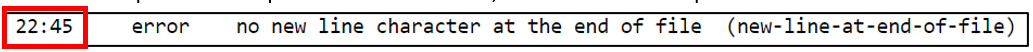
\includegraphics[width=16cm]{imagens/erroyaml.png}
	\caption{\label{fig:erroyaml} Exemplo de erro no yaml}
	\fonte{Os autores}
\end{figure}
\FloatBarrier

Elas representam, respectivamente, a linha e o caractere que apresentou o erro (ex: linha 22, caractere 45).


Esses foram os erros que conseguimos identificar conforme íamos tentando validar o nosso arquivo, então pode ser que há outros erros que não foram mapeados nessa postagem. 

Estamos abertos para a troca de experiências e esperamos ter ajudado :)

\section{Resumo de Atividades - Semana 11}
Na décima-primeira semana, entregamos e mostramos o documento final para o professor, que apontou alguns pontos de melhoria. Ele também alegou que o nosso arquivo equipe.yaml estava errado, pois não estava aparecendo no site da disciplina. Então fomos buscar mais a fundo sobre isso e conseguimos identificar os principais erros que podem aparecer na hora de validar um arquivo yaml. Assim, elaboramos um documento com esses principais erros, até mesmo para ajudar as próximas turmas da disciplina. 

No nosso checkpoint semanal, foi feito uma lista do que faltava para a aplicação ficar pronta e decidimos os próximos passos para cada integrante, que seria voltada para os ajustes no documento ou finalização da aplicação.

Além disso, ficamos sabendo que seríamos a primeira equipe a se apresentar (dia 26/07), então nos reunimos duas vezes para validar se estava tudo certo e também treinar para a apresentação final. 

Segue abaixo as atividades de cada integrante:

\begin{itemize}
\item André: fez a listagem de atividades e envio de anexos, a criação das conquistas, a entrega de atividades e de conquistas, o encerramento de turmas, correção na criação de atividades e o ranking
\item Bianca: ajustou o equipe.yaml, criou o documento dos erros do yaml, fez a apresentação do projeto e ajustou o documento final (segurança, escopo, manutenibilidade, métricas e apêndices)
\item Gustavo: fez a validação dos formulários de atividades e correções dos erros para a apresentação
\item Luiz: fez a geração do Latexdiff e os ajustes na documentação final (links de acesso, modelagem de dados, manutenibilidade, tecnologias e escopo)
\item Natan: gerou o vídeo do Gource, auxiliou na geração do Latexdiff e criou buscas dinâmicas dos registros da visão do administrador e do professor na tela do gestor
\item Patricia: fez os teste de alunos, de turmas, de conquistas e de atividades, o isolamento do firebase, a reorganização e a elaboração do roteiro de testes e montagem do backlog de correções
\end{itemize}

\section{Resumo de Atividades - Semana 12}
Na décima-segunda semana, apresentamos o nosso MVP para a banca. :)

Foi melhor que esperávamos, pois os pontos levantados pelos professores foram críticas construtivas que de fato estavam errados ou que irão agregar valor ao projeto. Desse modo, a semana foi destinada em discutir as melhorias para o documento final e para a aplicação.

Segue abaixo os pontos mais críticos citados:

\begin{itemize}
\item Aprofundamento da introdução e revisão de literatura;
\item Seguir a risca a metodologia ágil Scrum;
\item Ajustes no texto;
\item Boas práticas no código;
\item Melhor distribuição das tarefas.
\end{itemize}

No nosso checkpoint semanal, foi decidido os próximos passos para cada integrante, que seria:

\begin{itemize}
\item André: fazer um documento de boas práticas para o código
\item Bianca: cuidar da abordagem Scrum no projeto
\item Gustavo: ajustar as validações dos campos
\item Luiz: cuidar das alterações do documento para a entrega final
\item Natan: ajustar a internacionalização no código
\item Patricia: aumentar a cobertura de testes
\end{itemize}

Além disso, foi feito mais uma reunião, na qual o André passou as boas práticas mapeadas por ele para os demais integrantes, e também como ficaria o gerenciamento do projeto pelo GitHub.


\section{Resumo de Atividades - Semana 13}
Na décima-terceira semana, assistimos a apresentação da outra equipe e anotamos alguns pontos que também precisaríamos alterar no nosso projeto.

Como foi semana de provas das outras disciplinas, alteramos a data da nossa reunião semanal para domingo. Nessa reunião, abordamos os principais pontos de inconsistências para os ajustes finais do documento e da aplicação, e terminamos de ajustar o que faltava no nosso projeto.

Segue as atividades de cada integrante:

\begin{itemize}
\item André: implementou os tiers e fez os ajustes na aplicação
\item Bianca: fez os ajustes na documentação final
\item Gustavo: fez os ajustes na aplicação
\item Luiz: fez os ajustes na documentação final
\item Natan: fez os ajustes na aplicação
\item Patricia: aumentou a cobertura de teste
\end{itemize}
% ----------------------------------------------------------
\chapter{Protótipos das Telas}
\label{prototipos}
% ----------------------------------------------------------

\begin{figure}[htb]
    \centering
	
\includegraphics[width=16cm]{imagens/Geral-Login.png}
	\caption{\label{fig:login} Protótipo da Tela: Tela de Login}
	\fonte{Os autores}
\end{figure}
\FloatBarrier


\section{Visão do Administrador}

\begin{figure}[htb]
    \centering
	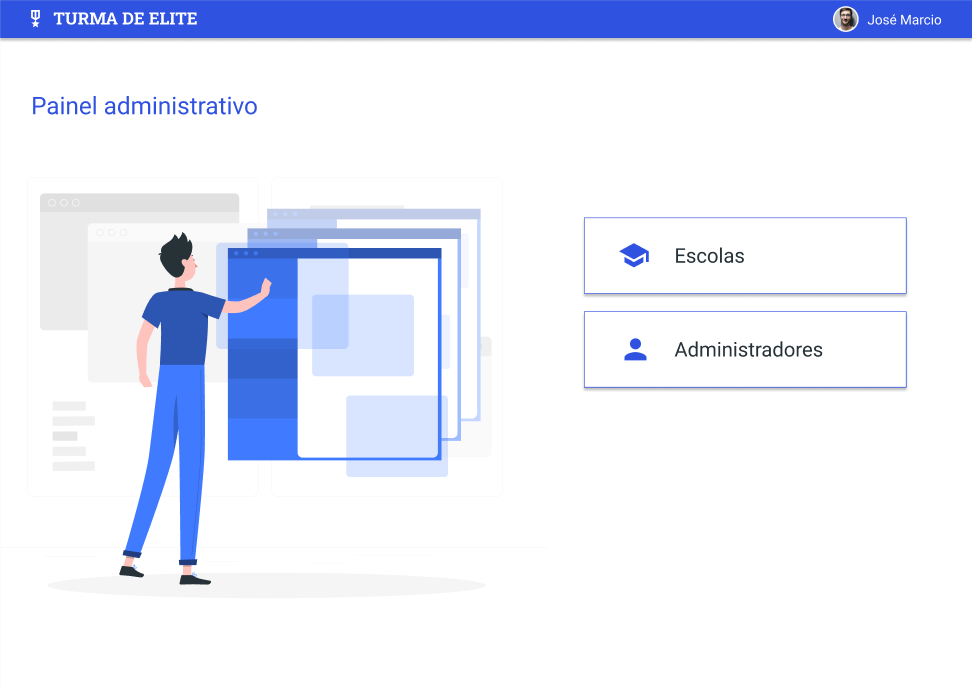
\includegraphics[width=16cm]{imagens/Administrador-PaginaInicial.png}
	\caption{\label{fig:administrador} Protótipo da Tela: Visão do Administrador - Página Inicial}
	\fonte{Os autores}
\end{figure}
\FloatBarrier

\begin{figure}[htb]
    \centering
	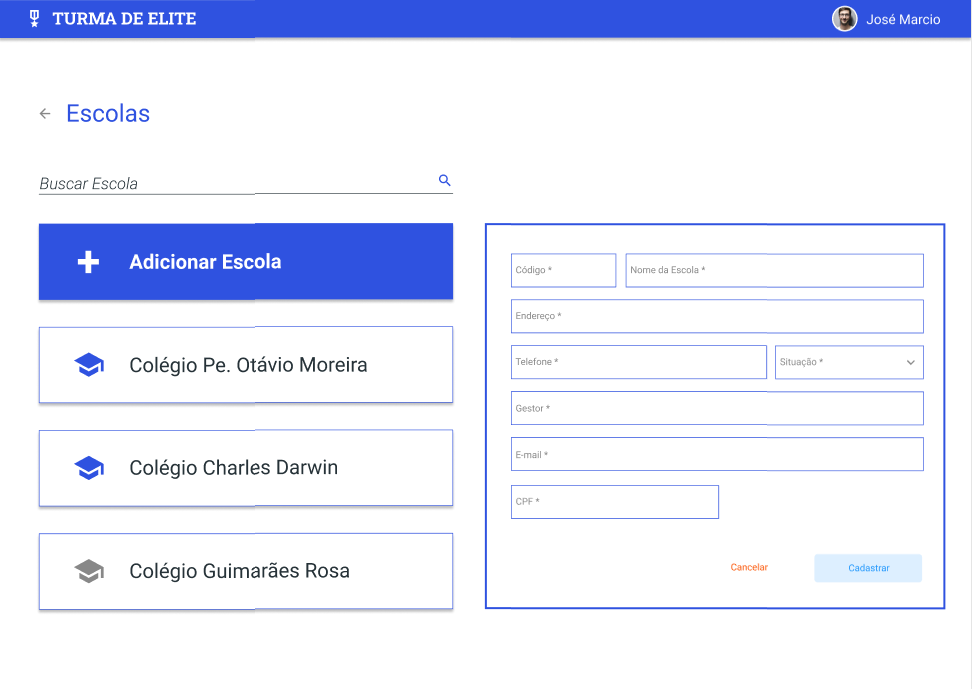
\includegraphics[width=16cm]{imagens/Administrador-CadastroEscola.png}
	\caption{\label{fig:cadastro-escola} Protótipo da Tela: Visão do Administrador - Cadastro de Escolas}
	\fonte{Os autores}
\end{figure}
\FloatBarrier

\begin{figure}[htb]
    \centering
	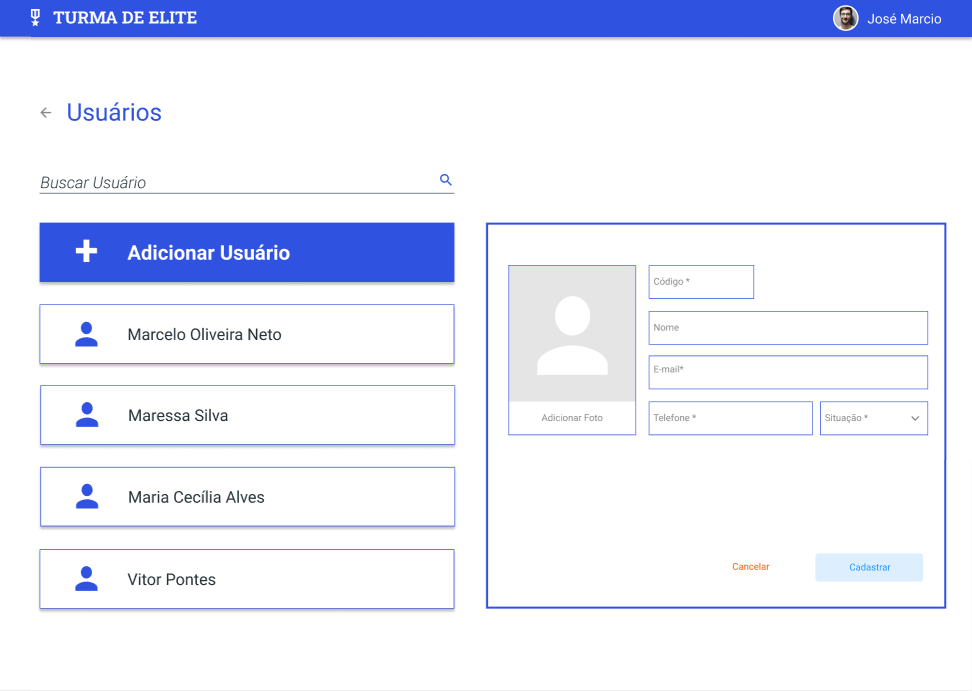
\includegraphics[width=16cm]{imagens/Administrador-CadastroUsuario.png}
	\caption{\label{fig:cadastro-usuário} Protótipo da Tela: Visão do Administrador - Cadastro de Usuários}
	\fonte{Os autores}
\end{figure}
\FloatBarrier


\section{Visão do Professor}

\begin{figure}[htb]
    \centering
	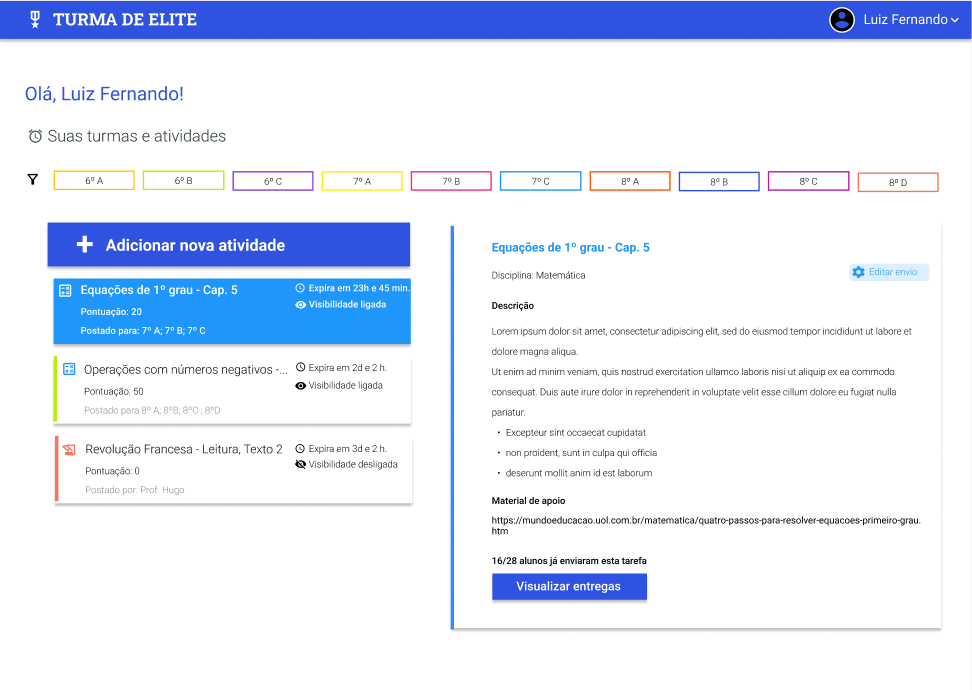
\includegraphics[width=16cm]{imagens/Professor-Atividades.png}
	\caption{\label{fig:atividades} Protótipo da Tela: Visão do Professor - Atividades}
	\fonte{Os autores}
\end{figure}
\FloatBarrier

\begin{figure}[htb]
    \centering
	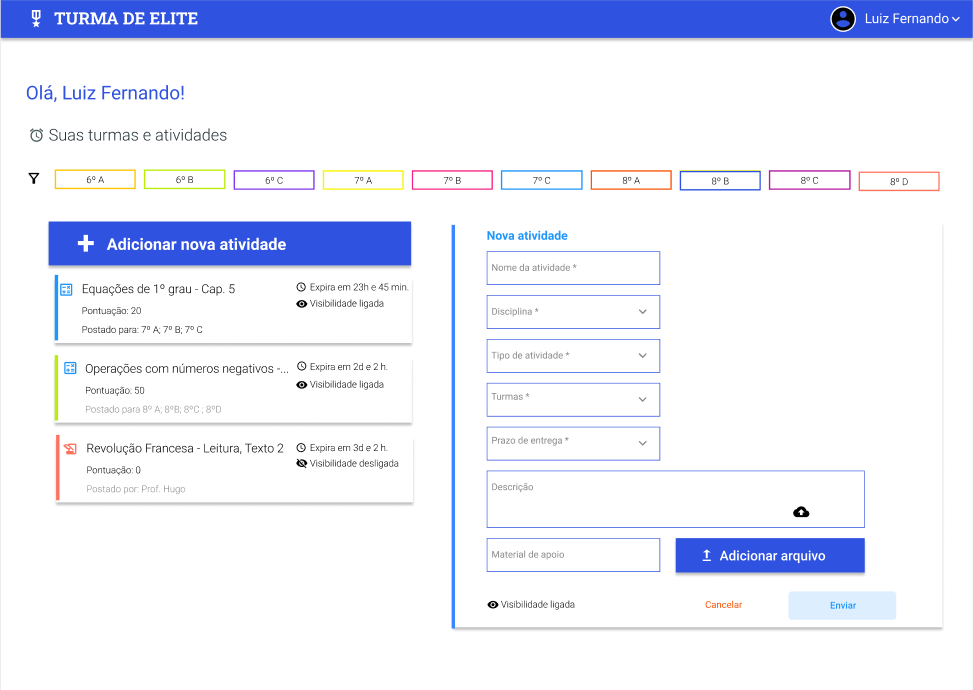
\includegraphics[width=16cm]{imagens/Professor-CadastroAtividades.png}
	\caption{\label{fig:professor} Protótipo da Tela: Visão do Professor - Cadastro de Atividades}
	\fonte{Os autores}
\end{figure}
\FloatBarrier


\section{Visão do Aluno}

\begin{figure}[htb]
    \centering
	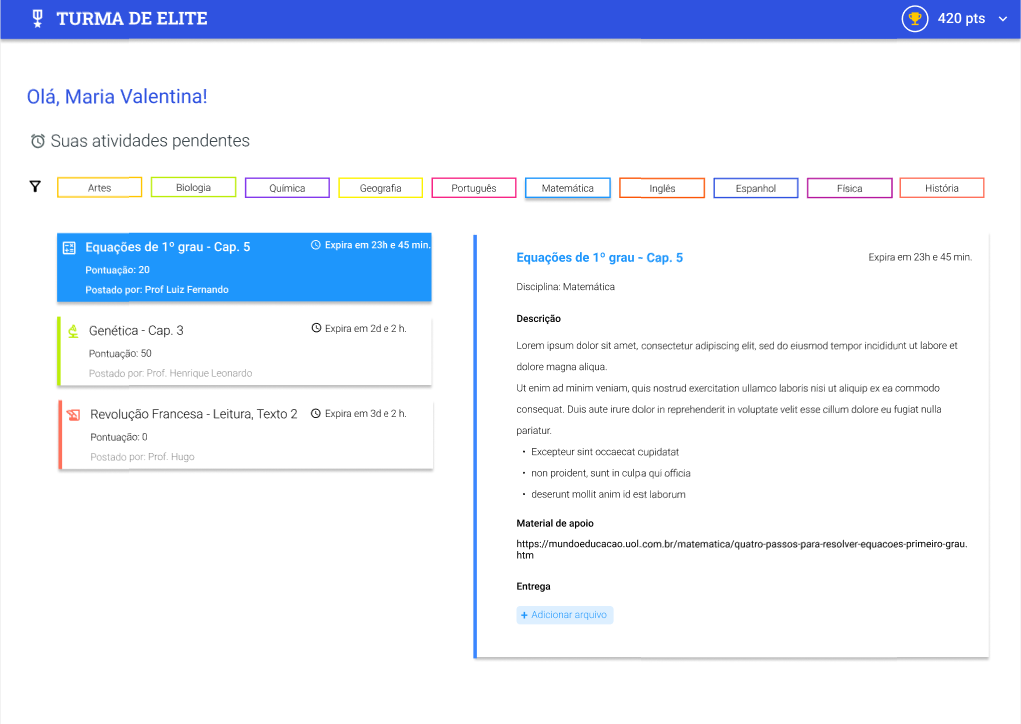
\includegraphics[width=16cm]{imagens/Aluno-Atividades.png}
	\caption{\label{fig:aluno} Protótipo da Tela: Visão do Aluno - Atividades}
	\fonte{Os autores}
\end{figure}
\FloatBarrier

\begin{figure}[htb]
    \centering
	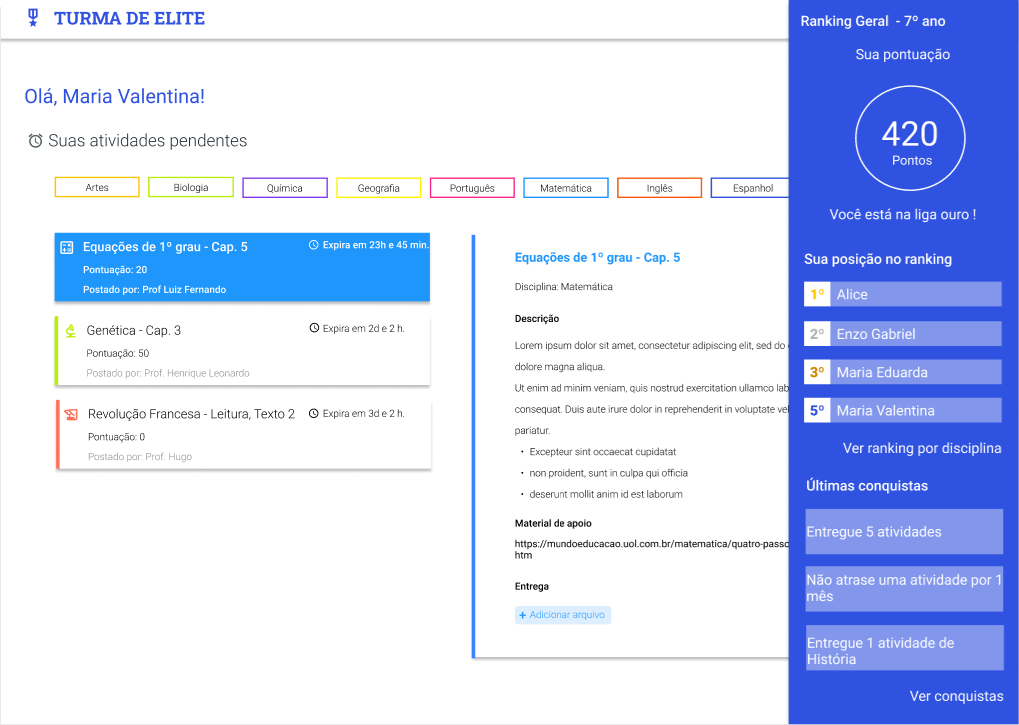
\includegraphics[width=16cm]{imagens/Aluno-MenuLateral.png}
	\caption{\label{fig:menu-lateral} Protótipo da Tela: Visão do Aluno - Menu Lateral}
	\fonte{Os autores}
\end{figure}
\FloatBarrier

\begin{figure}[htb]
    \centering
	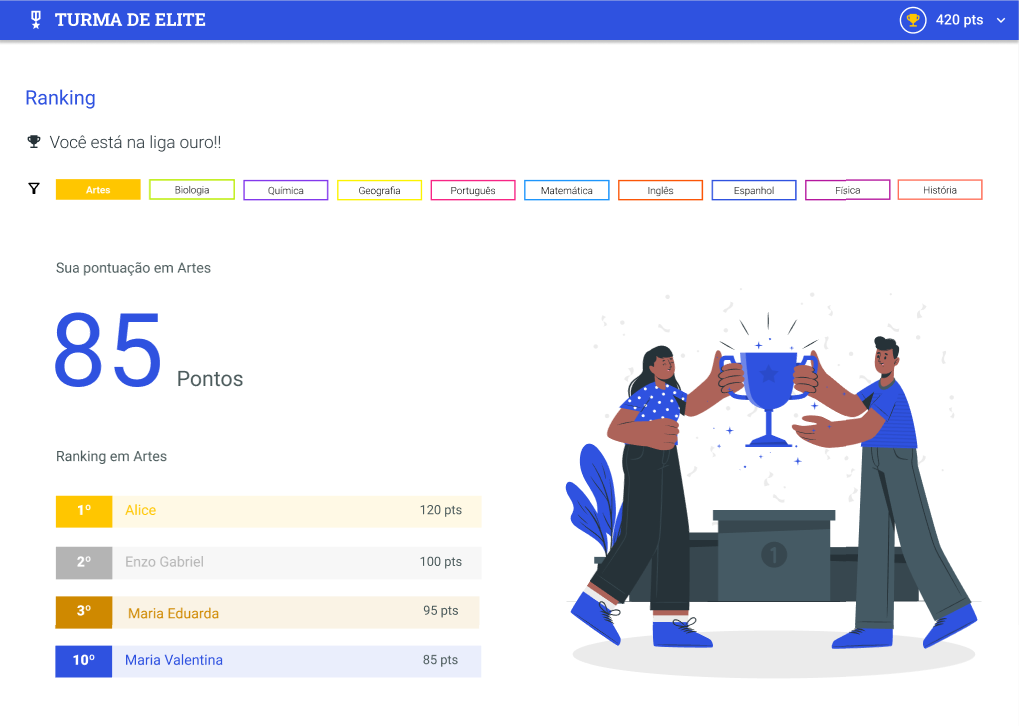
\includegraphics[width=16cm]{imagens/Aluno-Ranking.png}
	\caption{\label{fig:ranking} Protótipo da Tela: Visão do Aluno - Ranking}
	\fonte{Os autores}
\end{figure}
\FloatBarrier

\begin{figure}[htb]
    \centering
	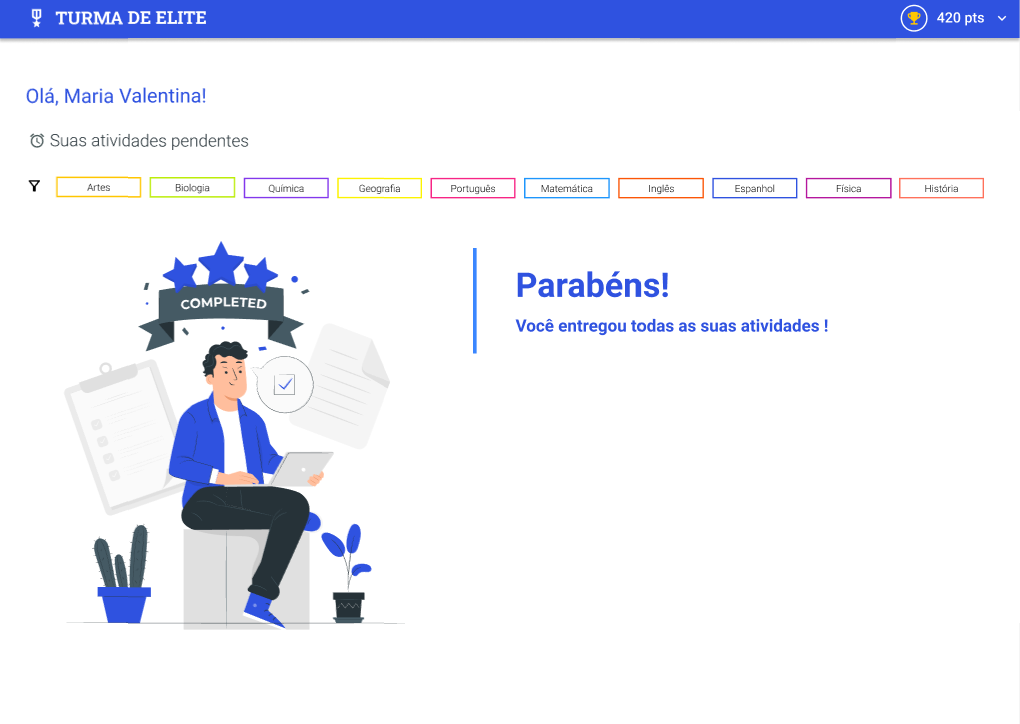
\includegraphics[width=16cm]{imagens/Aluno-Conquista.png}
	\caption{\label{fig:conquista} Protótipo da Tela: Visão do Aluno - Conquistas}
	\fonte{Os autores}
\end{figure}
\FloatBarrier


% ----------------------------------------------------------
\chapter{SSL Test - Back-end}
\label{ssltest-backend}
% ----------------------------------------------------------
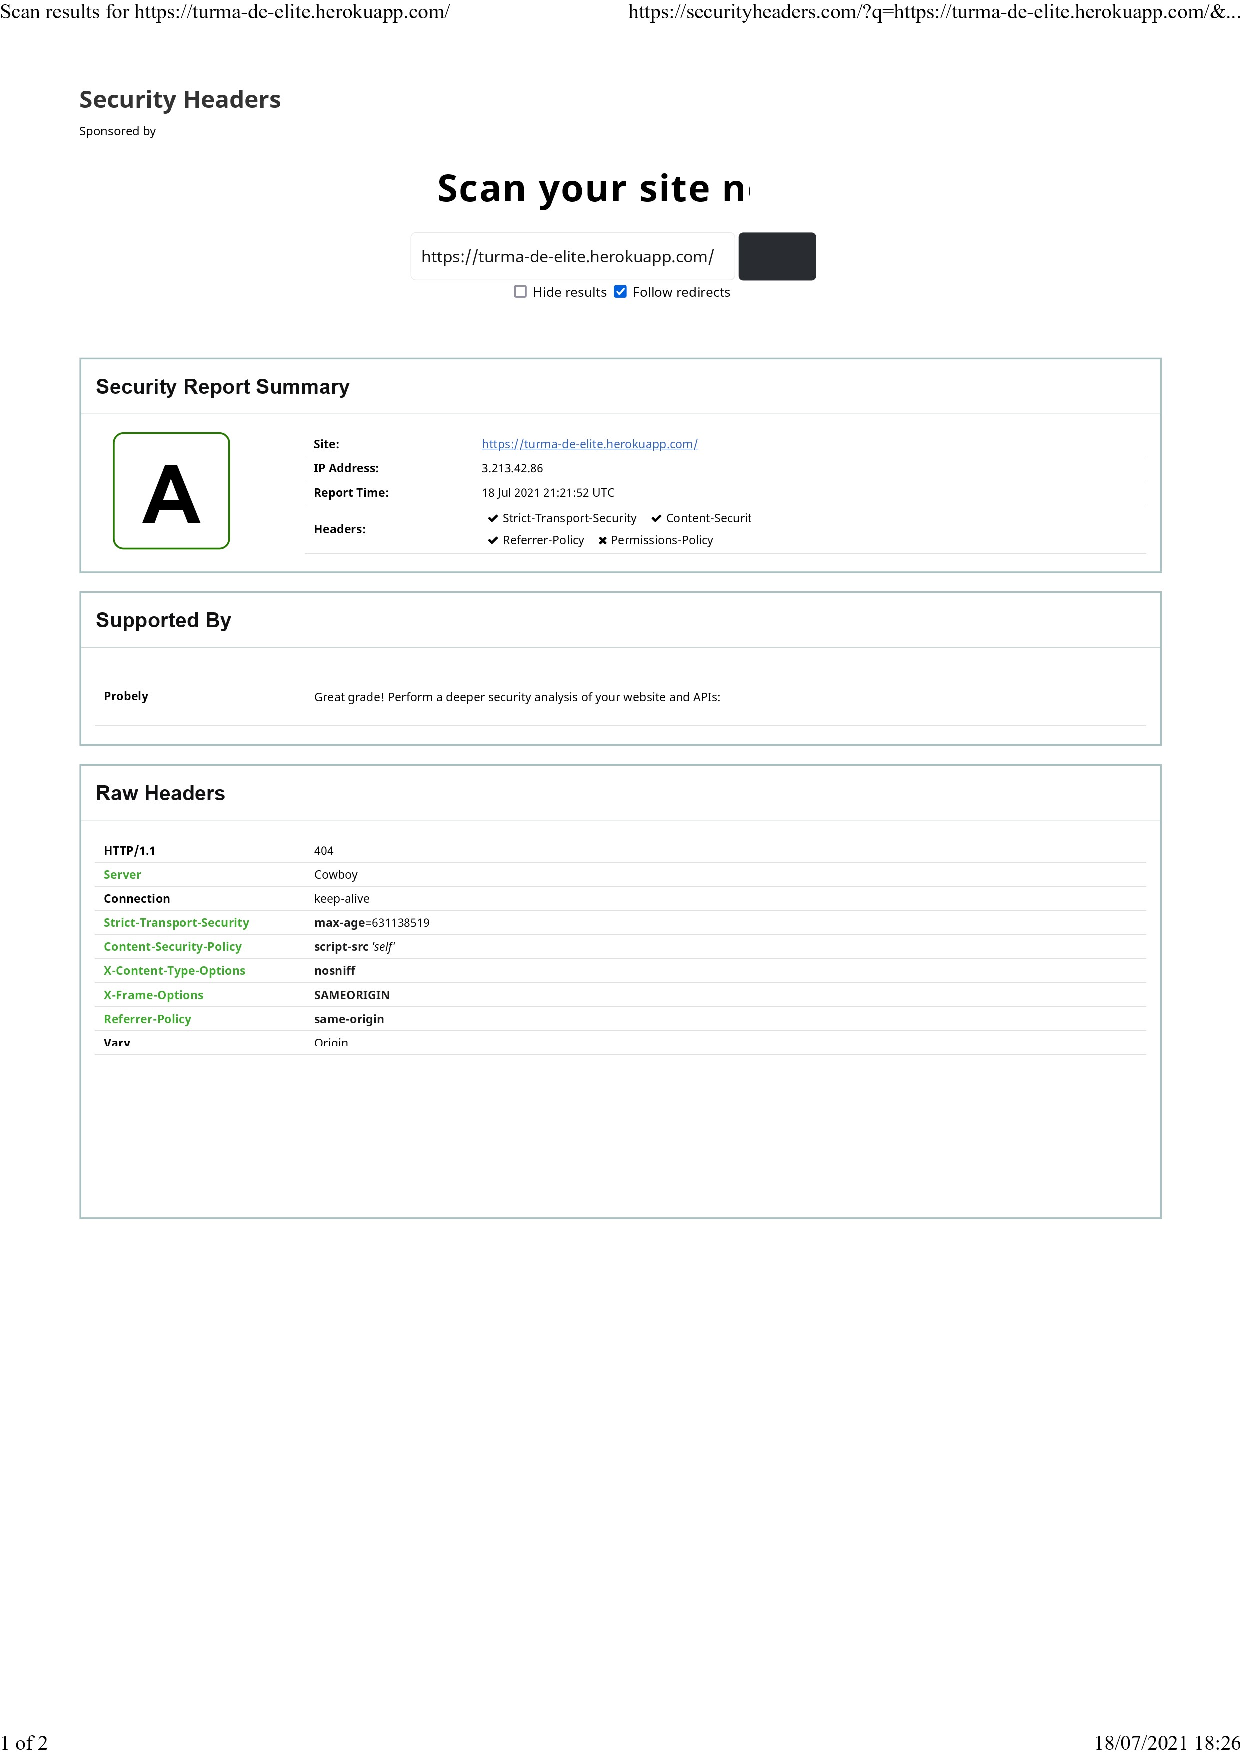
\includepdf[pages=-]{EntregaFinal/SECURITY_DOC.pdf}

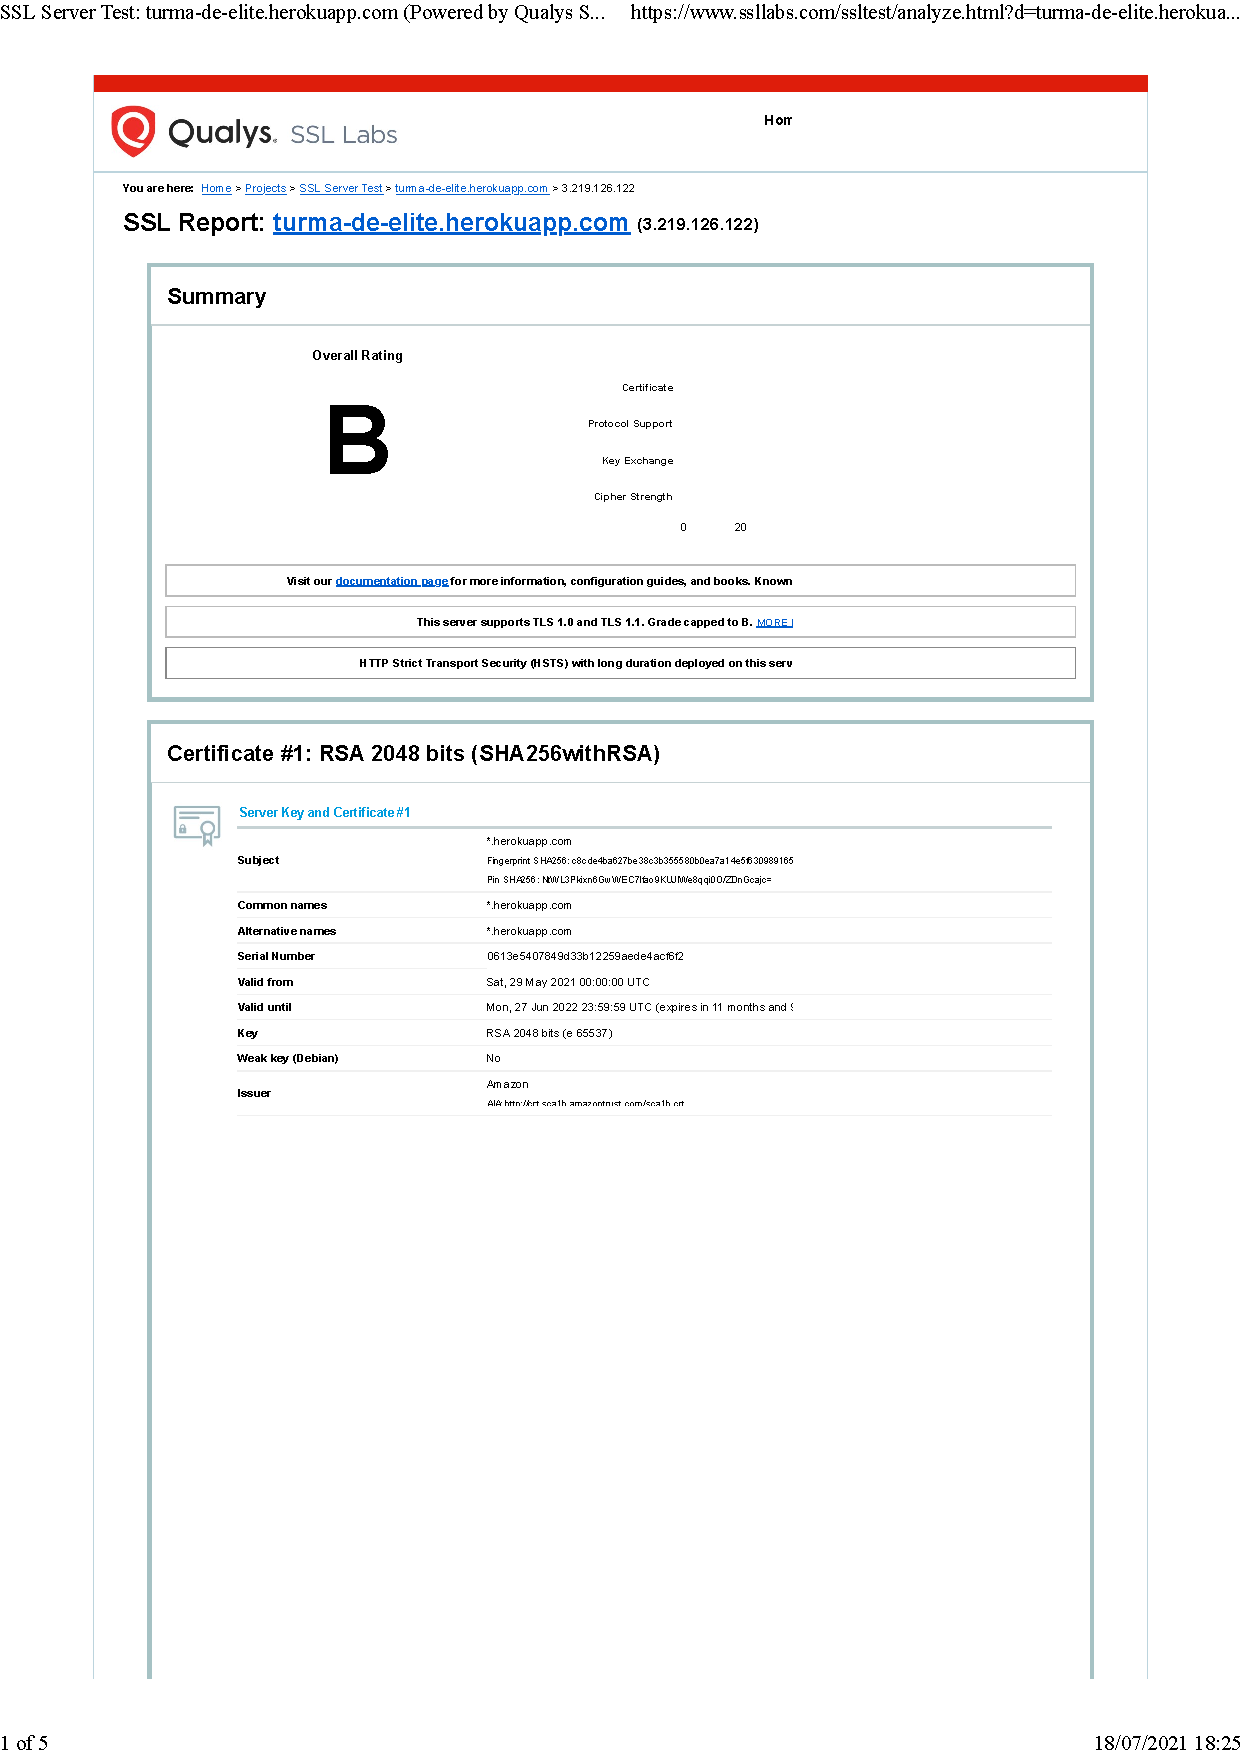
\includepdf[pages=-]{EntregaFinal/SSL_DOC.pdf}

% ----------------------------------------------------------
\chapter{SSL Test - Front-end}
\label{ssltest-frontend}
% ----------------------------------------------------------
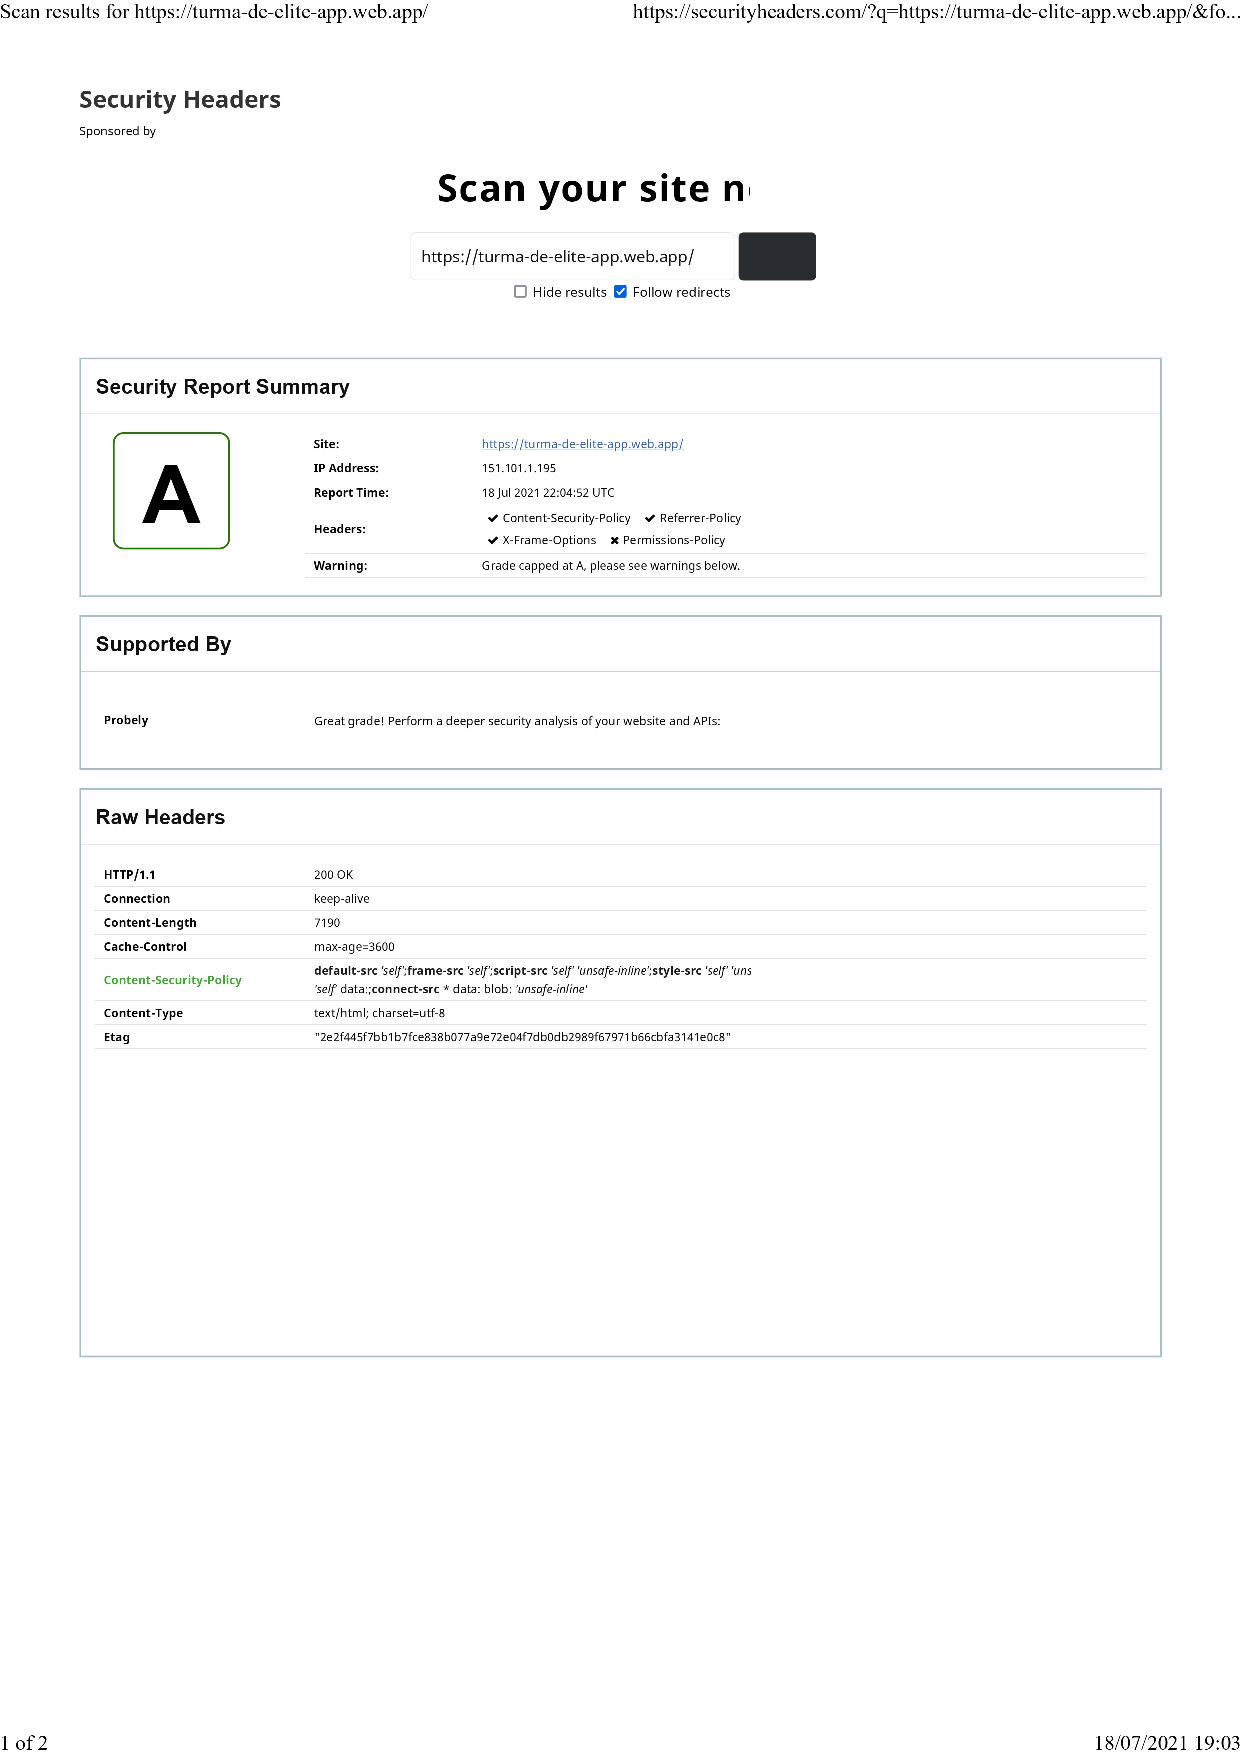
\includepdf[pages=-]{EntregaFinal/FRONT_END_SECURITY.pdf}

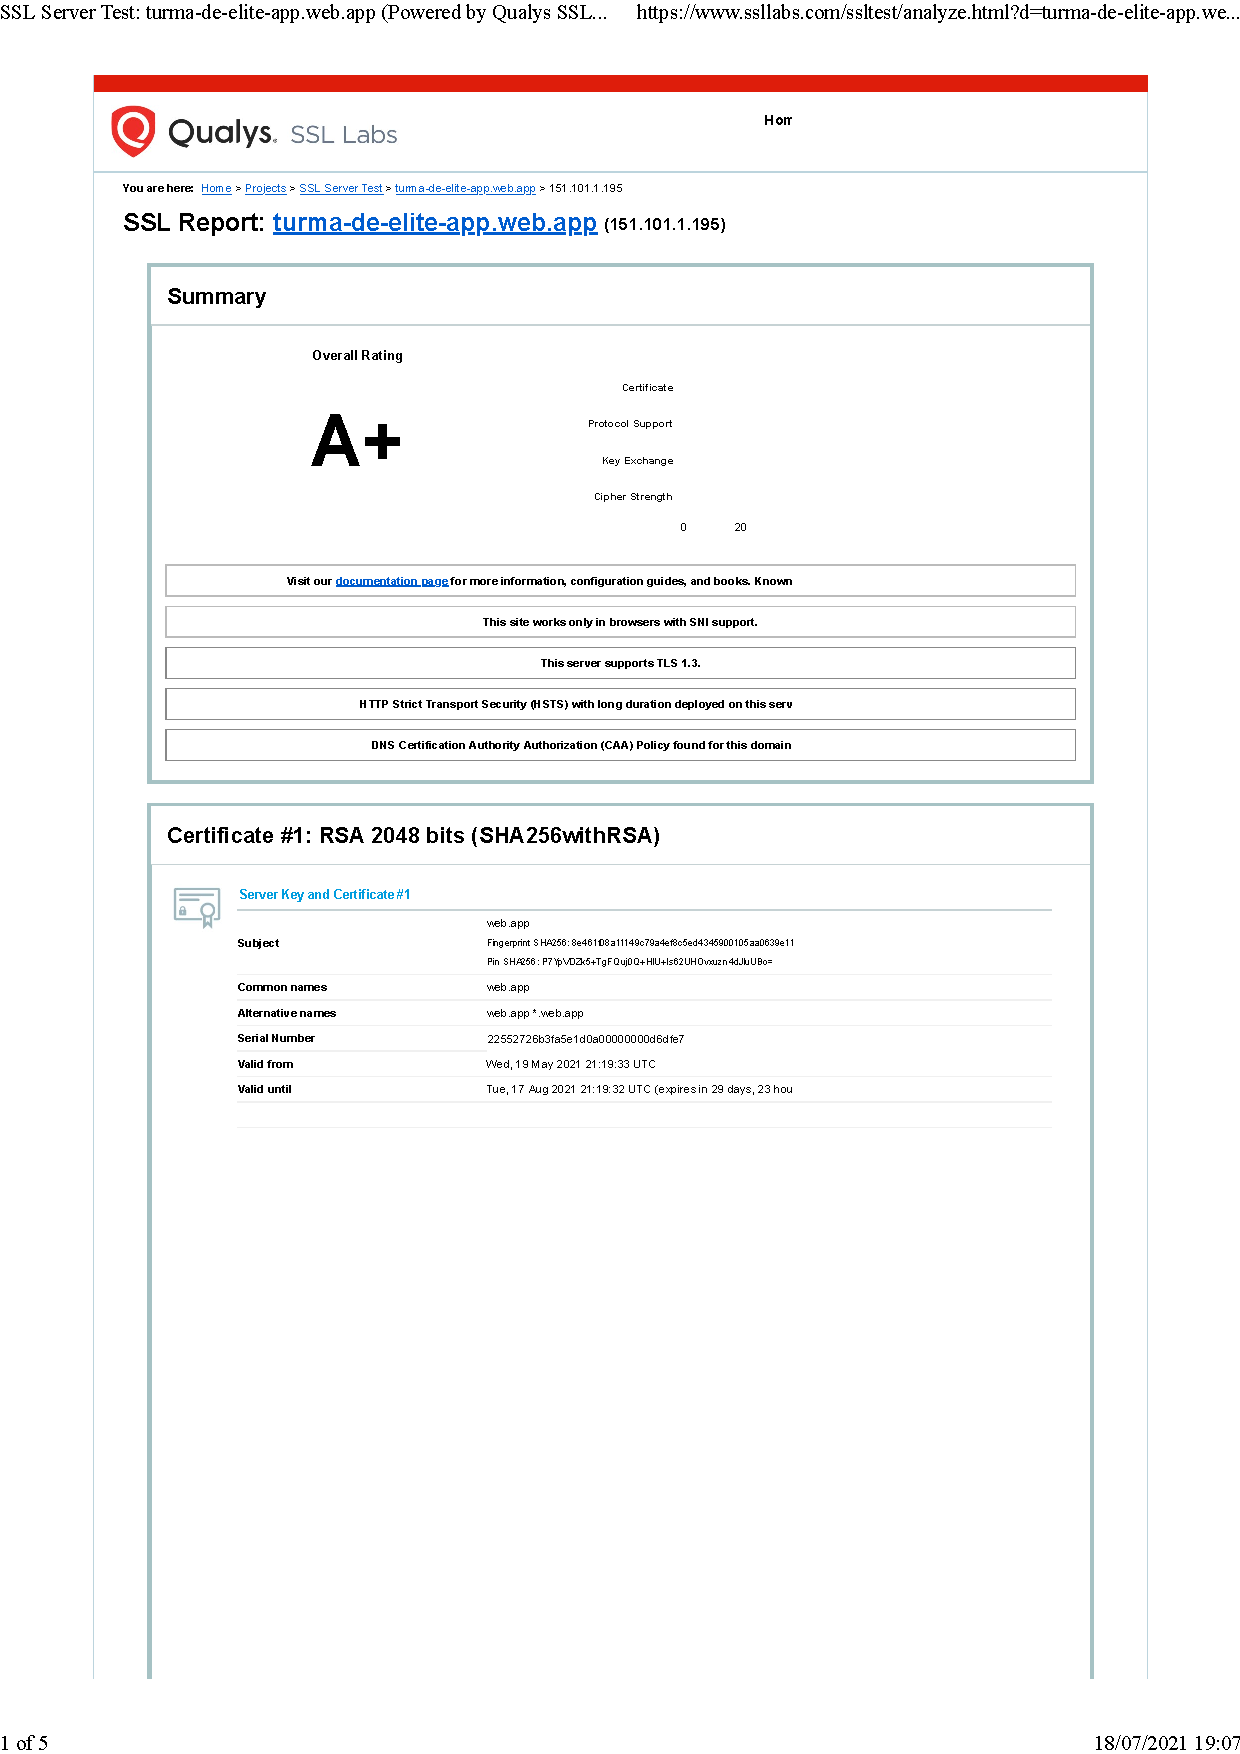
\includepdf[pages=-]{EntregaFinal/SSL_FRONT_DOC.pdf}
\end{apendicesenv}
% ---


\end{document}